\documentclass[UTF8]{ctexart}
\usepackage{fancyhdr}
\usepackage{lastpage}
\usepackage{layout}
\usepackage{amsmath}
\usepackage{ragged2e}
\usepackage{fancyhdr}
\usepackage{lastpage}
\usepackage{layout}
\usepackage{tikz}
\usepackage{amsmath}
\usepackage{graphicx}
\usepackage{subfigure}
\usepackage{bm}
\usepackage{fontspec}
\usepackage{inconsolata}
\usepackage{listings}
\newfontfamily\courier{Courier New}
\lstset{linewidth=1.1\textwidth,
        numbers=left, %设置行号位置
        basicstyle=\small\courier,
        numberstyle=\tiny\courier, %设置行号大小
        keywordstyle=\color{blue}\courier, %设置关键字颜色
        %identifierstyle=\bf,
        commentstyle=\it\color[cmyk]{1,0,1,0}\courier, %设置注释颜色
        stringstyle=\it\color[RGB]{128,0,0}\courier,
        %framexleftmargin=10mm,
        frame=single, %设置边框格式
        backgroundcolor=\color[RGB]{245,245,244},
        %escapeinside=``, %逃逸字符(1左面的键),用于显示中文
        breaklines, %自动折行
        extendedchars=false, %解决代码跨页时,章节标题,页眉等汉字不显示的问题
        xleftmargin=2em,xrightmargin=2em, aboveskip=1em, %设置边距
        tabsize=4, %设置tab空格数
        showspaces=false %不显示空格
        basicstyle=\small\courier
       }
\usepackage{array}
\usepackage{multirow}
\usepackage{booktabs}
\usepackage{caption}
\usepackage{paralist}
\usepackage{mathrsfs}
\usepackage{amsmath}
\usepackage{verbatim}
\usepackage{hyperref}
\usepackage{amsfonts}
\usepackage{algorithm}
%\usepackage{algorithmic}
\usepackage{algorithm}
\usepackage{algpseudocode}
\usepackage{graphicx}
\usepackage{float}
\usepackage{diagbox}
\renewcommand\contentsname{Contents}
\captionsetup[figure]{labelfont={bf},labelformat={default},labelsep=period,name={Figure.}}
%\pagestyle{empty}                   %不设置页眉页脚
\begin{document}
\title{\emph{Machine Learning: A Probabilistic Perspective} Solution Manual Version 2.1}
\author{Fangqi Li,\\ Shanghai Jiao Tong University,\\ P. R. China.}
\date{}
\maketitle
\tableofcontents
\newpage
\section{Preface}
\subsection{The Second Edition}
The tide of artificial intelligence (AI) has swept and reformed so many disciplines and pushed forward the borderline of the state-of-the-art.
Such situation has resulted in a positive feedback that drives even more attention and effort into the study and research of AI, together with more unsettled regret and pities.

I have participated in this study, with equal passion that any student who has not formed an exclusive view of the world should have when engaging in a booming subject.

It has been three years and four months since I started the first edition of this solution manual.
Although I have received no patron and have no intention of finding one, I received several grateful and advisory messages, from which I felt more pleased than having any of my technical papers published online.
For the convenience of them, I would gladly edit this manuscript again, be the time goes back to 2017.
In the second edition, I tried to be more concrete in deduction so readers can follow up easier.
Some graphical or numerical examples were provided to increase the overall readability.
At the beginning part of each chapter/after some exercises I left some remarks, which I thought that could be of help.

The purpose of this manuscript is, as its first edition, to complete the textbook \emph{Machine Learning, A Probabilistic Perspective} as a closed collection of knowledge as far as I could, and to save those who are lost in the ocean of deduction and symbols in ML, whom any talent mind could have become for some times in his/her course with this textbook.
I hope that this manuscript can help, be it ever so little, to any reader who purposedly or accidently finds it.

I personally take responsibility for any typo, or mistake in $\beta$-reductions.

Fangqi Li,

Shanghai Jiao Tong University,

Shanghai, P.R.China.

January the 4th, 2021.

Contact me by: \url{solour_lfq@sjtu.edu.cn} or \url{1524587011@qq.com}.

My homepage is at: \url{https://solour-lfq.github.io/}.

\newpage
\centerline{\Large{第二版序}}

这篇文档的主体由英文书写,这一方面是因为英文是学术上最泛用的语言,有利于本文档的传播;另一方面是我认为有能力阅读MLaPP原教材的中国学生、汉语母语学生基本上也能畅通无阻地阅读本文档中的英文。

希望中国学者和其他可以以中文为语言写作的学者一同努力,提升中文期刊、会议的质量和中文区科研院所的硬实力、影响力,让越来越多的学者乐于用中文叙述自己的观点。

第二版修订了第一版的一些文本问题,补充了第一版在习题推理上比较缺少的理念连接,同时增加了一些示例以提升可读性。文档内的所有排版错误、推导错误由我一人负责。

李方圻

上海交通大学

2021年1月4日

邮箱:\url{solour_lfq@sjtu.edu.cn},\url{1524587011@qq.com}。

主页:\url{https://solour-lfq.github.io/}。

\newpage
\subsection{The First Edition}
This document provides detailed solutions to almost all exercises in the textbook MLaPP from Chapter One to Chapter Twenty-one.
A reader is assumed to find support from this document when he/she is teaching himself/herself an introductory or advanced course with MLaPP.

There are two class for problems in MLaPP: theoretical ones and pratical ones.
We provide solution to most theoretical problems.
Practical problems, which are based on a Matlab toolbox, are beyond the scope of this document.

I started reading MLaPP after selecting a machine learning course, but I failed to find any free compiled solution manuals.
Although several publicly available projects have started working on it, the velocity has been too slow.
In the end, I hope that readers can provide comments and revise opinions. Apart from correcting the wrong answers, those who good at using MATLAB, Latex typesetting or those who are willing to participate in the improvement of the document are always welcome to contact me.

\

\

\

22/10/2017

Fangqi Li

Munich, Germany

\url{solour_lfq@sjtu.edu.cn}

\url{ge72bug@tum.de}

\newpage
\subsection{Updating log}
22/10/2017 First Chinese compilation.

02/03/2018 English version.

06/01/2020 The second edition begins.

\newpage
\section{Probability}
The probability theory for ML is usually a small subset of elementary probability.
More involved topics in probability begining from Kolmogorov's theory to martigale and Markov process is usually beyond the scope of an ordinary statistical ML textbook.
Readers are encouraged to refer to Shiryaev's \emph{Probability, 3rd edition}, whose first chapter gives a comprehensive summary of elementary probability theory.
For supplementary materials, readers can refer to Thomas's \emph{Elements of Information Theory} for a solid introduction.

\subsection{Probability are sensitive to the form of the question that was used to generate the answer}
Denote two children by $A$ and $B$.
The space of all experiment results, $\Omega$ is composed of:
$$\omega_{1}:A\text{ is a girl, },B\text{ is a girl},$$
$$\omega_{2}:A\text{ is a boy, },B\text{ is a boy},$$
$$\omega_{3}:A\text{ is a girl, },B\text{ is a boy},$$
$$\omega_{4}:A\text{ is a boy, },B\text{ is a girl}.$$
With uniform probability measure.
Denote the $\sigma$-algebra on $\Omega$ as $2^{\Omega}$.

In question (a), with the knowledge \emph{there is at least one boy}, $\Omega$ is modified into:
$$\Omega'=\left\{\omega_{2},\omega_{3},\omega_{4} \right\}.$$
The event that one child is a girl is $\left\{\omega_{3},\omega_{4} \right\}$, whose probability is:
$$\frac{|\left\{\omega_{3},\omega_{4} \right\}|}{|\Omega'|}=\frac{2}{3}.$$

In question (b), with the knowledge that $A$ is a boy, the reduced experiment space is:
$$\Omega''=\left\{\omega_{2},\omega_{4} \right\}.$$
Then the probability that $B$ is a girl is:
$$\frac{|\left\{\omega_{4} \right\}|}{|\Omega''|}=\frac{1}{2}.$$

The difference in the form of the question is reflected in that $\Omega$ is reduced to different forms and the desired events vary with our questions.

\subsection{Legal reasoning}
Given the assertation that the criminal has the special blood type, the space of all possibilities contains $800,000\times \frac{1}{100}=8,000$ samples.
A sample $\omega_{i}\in\Omega$ denotes that the $i$-th person with this blood type committed the crime.
Let the suspect be the $j$-th person with this special blood type, the event that he/she was the criminal is
$$\frac{1}{|\Omega|}=\frac{1}{8,000}.$$

For question (a): The probability that an innocent person has this blood type is almost 1\%, whose opposite event is \emph{the probability that an innocent person has another blood type}, which is 99\%.
This event is different from \emph{the suspect is the crimimal}.

For question (b): Justice is not measured by probability.
More evidence from forensics might increase this probability to unity or reduce it to zero.

\subsection{Variance of a sum}
Calculate this straightforwardly:
\begin{align}
\text{var}[X+Y]=&\mathbb{E}[(X+Y)^{2}]-\mathbb{E}^{2}[X+Y] \nonumber \\
=&\mathbb{E}[X^{2}]-\mathbb{E}^{2}[X]+\mathbb{E}[Y^{2}]-\mathbb{E}^{2}[Y]+2\mathbb{E}[XY]-2\mathbb{E}[X]\mathbb[Y] \nonumber \\
=&\text{var}[X]+\text{var}[Y]+2\text{cov}[X,Y].\nonumber
\end{align}
Using the definition of operators var, cov and the linearity of expectation should yield this result easily.

\subsection{Bayes rule for medical diagnosis}
Let ill and positive denote the event that you are infected and are tested positive for this disease respectively.
Let health denote the opposite event of ill.
Apply Bayes's rules:
\begin{align}
\text{Pr}(\text{ill}|\text{positive})=&\frac{\text{Pr}(\text{ill},\text{positive})}{\text{Pr}(\text{positive})}\nonumber \\
=&\frac{\text{Pr(ill)Pr(positive}|\text{ill)}}{\text{Pr(ill)Pr(positive}|\text{ill)+Pr(health)Pr(positive}|\text{health)}} \nonumber \\
=&0.0098 \nonumber
\end{align}

\subsection{The Monty Hall problem(The dilemma of three doors)}
The answer is (b).
Use $\text{prize}_{i}\text{, }\text{choose}_{i}\text{, }\text{open}_{i}$ to denote the event that the prize is in/the player chooses/the host opens the $i$-th box.
Apply Bayes's rules:
\begin{align}
\text{Pr}(\text{prize}_{1}|\text{choose}_{1},\text{open}_{3})=&\frac{\text{Pr}(\text{choose}_{1})\text{Pr}(\text{prize}_{1})\text{Pr}(\text{choose}_{3}|\text{prize}_{1},\text{choose}_{1})}{\text{Pr}(\text{choose}_{1})\text{Pr}(\text{open}_{3}|\text{choose}_{1})}\nonumber \\
=&\frac{\text{Pr}(\text{prize}_{1})\text{Pr}(\text{choose}_{3}|\text{prize}_{1},\text{choose}_{1})}{\text{Pr}(\text{open}_{3}|\text{choose}_{1})}\nonumber \\
=&\frac{\frac{1}{3}\cdot\frac{1}{2}}{\frac{1}{3}\cdot \frac{1}{2} + \frac{1}{3}\cdot 0 + \frac{1}{3} \cdot 1}=\frac{1}{3} \nonumber
\end{align}

In the last step we summarize over the potential location of the prize.
This is a classical example of anti-intuition results from probability.


\subsection{Conditional Independence}
In question (a), we have:
$$\text{Pr}(H|e_{1},e_{2})=\frac{\text{Pr}(H)\text{Pr}(e_{1},e_{2}|H)}{\text{Pr}(e_{1},e_{2})}$$

Thus the answer is (ii).

For question (b), we have the further decomposition:
$$\text{Pr}(H|e_{1},e_{2})=\frac{\text{Pr}(H)\text{Pr}(e_{1}|H)\text{Pr}(e_{2}|H)}{\text{Pr}(e_{1},e_{2})}$$

So both (i) and (ii) and sufficient obviously.
Moreover, we have:
\begin{align}
\text{Pr}(e_{1},e_{2})=& \sum_{H}\text{Pr}(e_{1},e_{2},H) \nonumber \\
=&\sum_{H} \text{Pr}(H)\text{Pr}(e_{1}|H)\text{Pr}(e_{2}|H) \nonumber
\end{align}
so (iii) is sufficint as well since we can calculate $p(e_{1},e_{2})$ from scratch.

\subsection{Pairwise independence does not imply mutual independence}
Consider three boolean variables $\xi_{1},\xi_{2},\xi_{3}$, $\xi_{1}$ and $\xi_{2}$ take values in 0 or 1 with equal possibility independently and $x_{3}=\text{XOR}(x_{1},x_{2})$.
It is easy to prove that $x_{3}$ is independent with $x_{1}$ or $x_{2}$, but given both $x_{1}$ and $x_{2}$, the value of $x_{3}$ is determined and thereby the mutual independence fails.
For a detailed examination, denote the space of experiment outcomes by
$$\Omega=\left\{00,01,10,11 \right\},$$
with the first component denote the value of $\xi_{1}$, the second is for $\xi_{2}$.
Then $\xi_{1}$ generates the $\sigma$-algebra:
$$\mathcal{F}_{1}=\left\{\emptyset,\Omega,\left\{00,01\right\},\left\{10,11\right\} \right\}.$$
$\xi_{2}$ generates:
$$\mathcal{F}_{2}=\left\{\emptyset,\Omega,\left\{00,10\right\},\left\{01,11\right\} \right\}.$$
$\xi_{3}$ generates:
$$\mathcal{F}_{3}=\left\{\emptyset,\Omega,\left\{00,11\right\},\left\{01,10\right\} \right\}.$$
One can easily check that each pair out of the triplet $\mathcal{F}_{1},\mathcal{F}_{2}$ and $\mathcal{F}_{3}$ is a pair of independent $\sigma$-algebra, hence meets the pairwise independence.

However, each pair out of the triplet $\mathcal{F}_{1},\mathcal{F}_{2}$ and $\mathcal{F}_{3}$ can span the entire $2^{\Omega}$.
Then we would have counter examples, e.g., consider
$$A=\left\{00,01\right\}\in\mathcal{F}_{1},$$
$$B=\left\{11\right\}\in\sigma(\xi_{2},\xi_{3}).$$
Then
$$\text{Pr}(A\cap B)=0\neq \text{Pr}(A)\cdot\text{Pr}(B)=\frac{1}{8}.$$
Hence the mutual independence does not hold.

This example comes from cryptography.
The only theoretical secure (defined by Shannon) encryption system is the one-pad cipher book.
With the message denoted by $m$ in binary code, the encryption is done by XOR $m$ with a binary key $k$ drawn from a cipher book.
The result is the cipher text $c$.
From a statistical point of view, $c$ is equally likely to be the ciphertext of any message, hence the adversary cannot break the security (since the cipher text can be equally understood as any message, so no specific message prevails).
But the encryption is a deterministic process (by using a stricy one-pad cipher book, this cipher is resistent to chosen-plaintext attack as well), so the mutual independence fails.

\subsection{Conditional independence iff joint factorizes}
We prove that (2.129) is tantamount to (2.130).
One direction is trivial by denoting:
$$g(x,z)=p(x|z)$$
$$h(y,z)=p(y|z)$$
Conversely, we have:
$$
\begin{aligned}
p(x|z)=&\sum_{y}p(x,y|z)  \\
=&\sum_{y}g(x,z)h(y,z)  \\
=&g(x,z)\sum_{y}h(y,z).
\end{aligned}
$$
And vice versa,
$$p(y|z)=h(y,z)\sum_{x}g(x,z).$$

Moreover, for any $z$:
\begin{align}
1=&\sum_{x,y}p(x,y|z) \nonumber \\
=&(\sum_{x}g(x,z))(\sum_{y}h(y,z)) \nonumber
\end{align}

Thus:
\begin{align}
p(x|z)p(y|z)=&g(x,z)h(y,z)(\sum_{x}g(x,z))(\sum_{y}h(y,z)) \nonumber \\
=&g(x,z)h(y,z) \nonumber \\
=&p(x,y|z) \nonumber
\end{align}

\subsection{Conditional independence}
For question (a), the antecedent $(X\perp W|Z,Y)$ means that $\forall x\in\sigma(X)$, $\forall w\in\sigma(W)$ and $\forall v\in\sigma(Y,Z)$ we have
$$\text{Pr}(x\cap w|v)=\text{Pr}(x|v)\cdot\text{Pr}(w|v).$$
The antecedent $(X\perp Y|Z)$ can be translated to that $\forall x\in\sigma(X)$, $\forall y\in\sigma(Y)$ and $\forall z\in\sigma(Z)$,
$$\text{Pr}(x\cap y|z)=\text{Pr}(x|z)\cdot\text{Pr}(y|z).$$
What we desire to obtain is $\forall x\in\sigma(X)$, $\forall w\in\sigma(W)$ and $\forall z\in\sigma(Z)$,
$$\text{Pr}(x\cap w|z)=\text{Pr}(x|z)\cdot\text{Pr}(w|z).$$
This is obviously correct by having $v$ in the first equation taking values in $\sigma(Z)$ solely.
Since $\sigma(Z)\subset \sigma(Y,Z)$.

For question (b), we have the premises: $\forall x\in\sigma(X)$, $\forall y\in\sigma(Y)$, $\forall z \in\sigma(Z)$ and $\forall w\in\sigma(W)$:
$$\text{Pr}(x\cap y|z)=\text{Pr}(x|z)\cdot\text{Pr}(y|z).$$
$$\text{Pr}(x\cap y|w)=\text{Pr}(x|w)\cdot\text{Pr}(y|w).$$
The desired result if $\forall v\in\sigma(Z,W)$,
$$\text{Pr}(x\cap y|v)=\text{Pr}(x|v)\cdot\text{Pr}(y|v).$$
Let $x$ and $y$ be two disjoint events, $z$ and $w$ be another pair of disjoints, and none of $x\cap z,x\cap w, y\cap z,y\cap w$ is empty w.r.t. the underlying probability measure.
Finally, let $v=w\cup z$.
One can then check that the equation above does not hold for this setting, hence the deduction in (b) is false.

In fact, (b) is intuitively false.
A straightforward example is a cryptography example: group signature with three participants.
The group signature is a protocal for encryption/verfication that ensures a series of security requirements including:
\begin{itemize}
\item Any one participant soly cannot pass the verification.
\item Two participant can pass the verification.
\end{itemize}
For example, let Alice and Bob each hold a half of the secret key denoted by $Z$ and $W$ respectively, $Y$ denotes the ciphertext, and $X$ denotes the plaintext.
A good group encryption would meet both antecedents in (b) but fails the conclusion.
An example of a naive group signature is to use a quadratic function as the secret key:
$$f(t)=x\cdot t^{2}+y\cdot t +c.$$
And provide two different points $z=(t_{1},f_{1})$, $w=(t_{2},f_{2})$ from $f$ to Alice and Bob.
It is obvious that both antecedents in (b) are satisfied (by correctly translating the density) since the value of $x$ yields no information about $y$.
However, given both $z$ and $w$ then $y$ is a determinstic function of $x$:
$$y=\frac{f_{1}-f_{2}}{t_{1}-t_{2}}-x\cdot(t_{1}+t_{2}),$$
and the independence no longer holds.
Note that a third participant is necessary to reveal the entire secret key $(x,y,c)$.
In practice, the calculation is usually done on an algebraic field/group, e.g. the elliptic curves, to deal with the problem with the density of $x,y,c$ which is usually not uniform in the real number field.

\subsection{Deriving the inverse gamma density}
According to the change of variables formula:
$$p(y)=p(x)|\frac{\text{d}x}{\text{d}y}|.$$
We have:
\begin{align}
\text{IG}(y)=&\text{Ga}(x)\cdot y^{-2} \nonumber \\
=&\frac{b^{a}}{\Gamma(a)}(\frac{1}{y})^{(a-1)+2}e^{-\frac{b}{y}} \nonumber \\
=&\frac{b^{a}}{\Gamma(a)}(y)^{-(a+1)}e^{-\frac{b}{y}}. \nonumber
\end{align}

The change of variables formula is a simplified version of Lebesgue-Rikdon Theorem, which formally address the transform between probability measures defined on the same space.
In the simplified version, we take the existence of the derivative $\frac{\text{d}x}{\text{d}y}$ for granted.
In the general case, such differential is obtained by taking the limit of simple functions that meet the dominance condition.
In fact, the Lebesgue Theorem was developed to properly define the \emph{differential of one probability measure w.r.t. another probability measure}.
The derived general differential is usually denoted by $\frac{\text{d}\mu_{1}(x)}{\text{d}\mu_{2}(x)}$ where $\mu_{i}$ are probability measures.


\subsection{Normalization constant for a 1D Gaussian}
We have:
$$
\begin{aligned}
C&=\int_{0}^{2\pi}\int_{0}^{\infty}r\cdot\exp\left\{-\frac{r^{2}}{2\sigma^{2}} \right\}\text{d}r\text{d}\theta\\
&=2\pi\sigma^{2}\cdot\int_{0}^{\infty}\exp\left\{-u\right\}\text{d}u\\
&=2\pi\sigma^{2}.
\end{aligned}
$$
For multivariate Gaussian, the trick is to diagonalize the covariance matrix and integral each components independently.


\subsection{Expressing mutual information in terms of entropies}
We have:
\begin{align}
I(X;Y)=&\sum_{x,y}p(x,y) \log \frac{p(x,y)}{p(x)p(y)} \nonumber \\
=&\sum_{x,y}p(x,y)\log \frac{p(x|y)}{p(x)} \nonumber \\
=&\sum_{x,y}p(x,y)\log p(x|y) - \sum_{x}(\sum_{y}p(x,y))\log p(x) \nonumber \\
=&-H(X|Y)+H(X) \nonumber
\end{align}

Inversing $X$ and $Y$ yields another formula.
One can proceed to show that $I(X;Y)=H(X)+H(Y)-H(X,Y)$.

\subsection{Mutual information for correlated normals}
We have:
\begin{align}
I(X_{1};X_{2})=&H(X_{1})-H(X_{1}|X_{2}) \nonumber \\
=&H(X_{1})+H(X_{2})-H(X_{1},X_{2}) \nonumber \\
=&\frac{1}{2}\log 2\pi\sigma^{2}+\frac{1}{2}\log 2\pi\sigma^{2}+\frac{1}{2}\log (2\pi)^{2}\sigma^{4}(1-\rho^{2}) \nonumber \\
=&-\frac{1}{2}\log (1-\rho^{2}) \nonumber
\end{align}

Here we incorporate a comprehensive deduction on (2.138) and (2.139), which shall not be taken for granted.
The differential entropy for a 1D-Gaussian with density function:
$$p(x)=\frac{1}{\sqrt{2\pi\sigma^{2}}}\exp\left\{-\frac{x^{2}}{2\sigma^{2}} \right\}$$
is
$$
\begin{aligned}
&-\int\frac{1}{\sqrt{2\pi\sigma^{2}}}\exp\left\{-\frac{x^{2}}{2\sigma^{2}} \right\} \ln\left(\frac{1}{\sqrt{2\pi\sigma^{2}}}\exp\left\{-\frac{x^{2}}{2\sigma^{2}} \right\} \right) \text{d}{x}\\
&=\ln(\sqrt{2\pi\sigma^{2}})+\frac{1}{2\sigma^{2}}\mathbb{E}[x^{2}]\\
&=\frac{1}{2}\ln(2\pi e\sigma^{2}).
\end{aligned}
$$
For the multi-dimensional case, we begin by diagonalizing the covariance matrix/decoupling the components and integrating along each independent component.
Under this new set of coordinates $v_{1},\cdots,v_{d}$, the logarithm of the density can be decomposed into
$$C+\sum_{i=1}^{d}-\frac{v_{i}^{2}}{2\sigma_{i}^{2}},$$
where $\sigma^{2}_{i}$ is the $i$-th diagonal component in the transformed covariance matrix.
The product of all diagonal components is exactly $\text{det}\Sigma$, hence proving (2.138).

\subsection{A measure of correlation}
For question (a), we only have to borrow the conclusion from Exercise 2.12.:
\begin{align}
r=&1-\frac{H(Y|X)}{H(X)}=\frac{H(X)-H(Y|X)}{H(X)} \nonumber \\
=&\frac{H(Y)-H(Y|X)}{H(X)} \nonumber \\
=&\frac{I(X;Y)}{H(X)} \nonumber
\end{align}

For question (b), we have $0 \leq r \leq 1$ in question b for $I(X;Y) \geq 0$ and $H(X|Y) \geq 0$.

For question (c), $r=0$ iff $X$ and $Y$ are independent so the distance between $p(x,y)$ and $p(x)\cdot p(y)$ is zero regarding KL-divergence.

For question (d), $r=1$ iff $X$ is determined by, but not necessarily equal to, $Y$.

\subsection{MLE minimizes KL divergence to the empirical distribution}
Expand the KL divergence:
\begin{align}
\theta=&\arg\min_{\theta}\left\{ \mathbb{KL}(p_{\text{emp}}||q(\theta)) \right\} \nonumber \\
=&\arg\min_{\theta}\left\{ \mathbb{E}_{p_{\text{emp}}}[\log \frac{p_{\text{emp}}}{q(\theta)}] \right\} \nonumber \\
=&\arg\min_{\theta}\left\{ -H(p_{\text{emp}}) - \sum_{\textbf{x}\in \text{dataset}}(\log q(\textbf{x};\theta)) \right\} \nonumber \\
=&\arg\max_{\theta}\left\{ \sum_{\textbf{x}\in \text{dataset}} \log p(\textbf{x};\theta)\right\} \nonumber
\end{align}

We use the weak law of large numbers in the third step and drop the entropy of empirical distribution, which is independent of $\theta$, in the last step.
The other direction of optimization is $\arg\min_{\theta}\left\{\mathbb{KL}(q(\theta)||p_{\text{emp}}) \right\}$.
It contains an expectation term w.r.t. $q(\theta)$ and is harder to solve.

\subsection{Mean, mode, variance for the beta distribution}
Firstly, we derive the mode for beta distribution by differentiating the pdf:
$$\frac{\text{d}}{\text{d}x}x^{a-1}(1-x)^{b-1}=[(1-x)(a-1)-(b-1)x]x^{a-2}(1-x)^{b-2}$$

Setting this to zero yields:
$$\text{mode}=\frac{a-1}{a+b-2}$$

Secondly, derive the moment in beta distribution:
\begin{align}
\mathbb{E}[x^{N}]=&\frac{1}{B(a,b)}\int x^{a+N-1}(1-x)^{b-1} dx \nonumber \\
=&\frac{B(a+N,b)}{B(a,b)} \nonumber \\
=&\frac{\Gamma(a+N)\Gamma(b)}{\Gamma(a+N+b)} \frac{\Gamma(a+b)}{\Gamma(a)\Gamma(b)} \nonumber
\end{align}

Setting $N=1,2$:
$$\mathbb{E}[x]=\frac{a}{a+b}$$
$$\mathbb{E}[x^{2}]=\frac{a(a+1)}{(a+b)(a+b+1)}$$

Where we have used the properties of the Gamma function.
Finally:
$$\text{mean}=\mathbb{E}[x]=\frac{a}{a+b}$$
$$\text{variance}=\mathbb{E}[x^{2}]-\mathbb{E}^{2}[x]=\frac{ab}{(a+b)^{2}(a+b+1)}$$

\subsection{Expected value of the minimum}
Let $m$ denote the location of the left most point, we have:
\begin{align}
p(m>t)=&p([X>t] \text{ and } [Y>t])\nonumber \\
=&p(X>t)p(Y>t) \nonumber \\
=&(1-t)^{2} \nonumber
\end{align}

Therefore:
\begin{align}
\mathbb{E}[m]=&\int_{0}^{1} t\cdot p(m=t)\text{d}t \nonumber \\
=&\int_{0}^{1} p(m>t)\text{d}t \nonumber \\
=&\int_{0}^{1}(1-t)^{2}\text{d}t \nonumber \\
=&\frac{1}{3}\nonumber
\end{align}
For the second equation, note that:
$$p(m\geq t)=\int_{t}^{1-t}p(m=t')\text{d}t',$$
therefore
$$\int_{0}^{1}\int_{t}^{1-t}p(m=t')\text{d}t'\text{d}t=\int_{0}^{1}\int_{0}^{t'}p(m=t')\text{d}t\text{d}t'=\int_{0}^{1}t\cdot p(m=t')\text{d}t'.$$

There are perhaps more intuitive solutions to this problem, for example, plotting the value of $X$, $Y$ and $\min(X,Y)$ into one graph:
\begin{figure}[htbp]
\centering
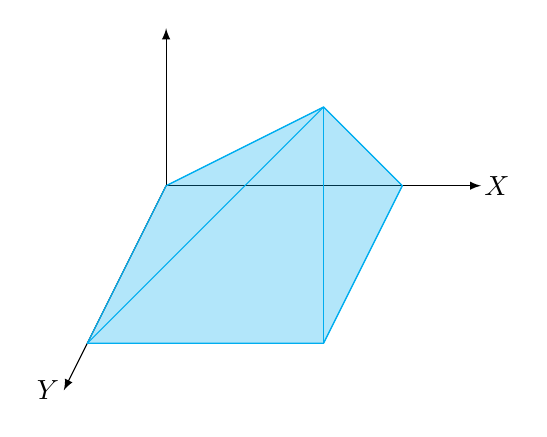
\begin{tikzpicture}
\draw [-latex] (0,0)--(0,2);
\draw [-latex] (0,0)--(4,0);
\draw [-latex] (0,0)--(-1.3,-2.6);
\draw [cyan] (0,0)--(2,1);
\draw [cyan] (3,0)--(2,1);
\draw [cyan] (-1,-2)--(2,1);
\draw [cyan] (3,0)--(2,-2);
\draw [cyan] (-1,-2)--(2,-2);
\draw [cyan] (2,-2)--(2,1);
\filldraw [cyan,fill opacity=0.3] (0,0)--(2,1)--(3,0)--(2,-2)--(-1,-2)--(0,0);
\node at (4.2,0) {$X$};
\node at (-1.5,-2.6) {$Y$};
\end{tikzpicture}
\caption{Exercise 2.17, P1.}
\label{figure:2.1}
\end{figure}
The height of the cyan pyramid at $(x,y)$ marks the value of $\min(x,y)$, so the expectation of the statistics equals the average height, in this case also the volume of the pyramid, $\frac{1}{3}$.
One can also graphically compute the average distance between $X$ and $Y$ from the following plot:
\begin{figure}[htbp]
\centering
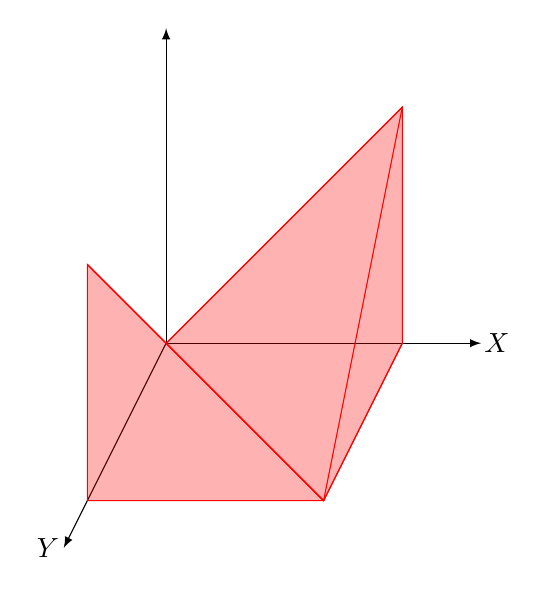
\begin{tikzpicture}
\draw [-latex] (0,0)--(0,4);
\draw [-latex] (0,0)--(4,0);
\draw [-latex] (0,0)--(-1.3,-2.6);
\draw [red] (0,0)--(2,-2);
\draw [red] (0,0)--(3,3);
\draw [red] (3,3)--(2,-2);
\draw [red] (3,0)--(2,-2);
\draw [red] (3,0)--(3,3);
\draw [red] (2,-2)--(-1,-2);
\draw [red] (-1,-2)--(-1,1);
\draw [red] (0,0)--(-1,1);
\draw [red] (-1,1)--(2,-2);
\filldraw [red,fill opacity=0.3] (0,0)--(3,3)--(3,0)--(2,-2)--(0,0);
\filldraw [red,fill opacity=0.3] (-1,-2)--(2,-2)--(-1,1)--(-1,-2);
\node at (4.2,0) {$X$};
\node at (-1.5,-2.6) {$Y$};
\end{tikzpicture}
\caption{Exercise 2.17, P2}
\end{figure}
Since the average distance between $X$ and $Y$ is $\frac{1}{3}$, so is that between $\min(X,Y)$ and $\max(X,Y)$.
Moreover, we have $\mathbb{E}[\min(X,Y)+\max(X,Y)]=\mathbb{E}[X]+\mathbb{E}[Y]=1$, hence $\min(X,Y)=\frac{1}{3}$.

However, the graphical method, although entertaining and inspiring, should not be considered as an reliable option in proving probability properties.
The dependency can complicate the underlying topology (e.g., the $X-Y$ plance might have another geometry other than the Euclidean one, if $X$ and $Y$ are not independent), resulting in confusions and fallacies.

For example, if $X$ is subject to a uniform distribution on $[0,1]$ while $Y$ is uniformly distributed in $[\max(0,X-0.2),\min(1,X+0.2)]$.
Then the pyramid in Fig. \ref{figure:2.1} is left with the region along the diagonal line in $X$-$Y$ plane.
This generalization is insignificant since it only changes the region where the integral shall be done.

Consider the case where $X$ and $Y$ are independent random variables subject to truncated Gaussian centered at $\frac{1}{2}$ on $[0,1]$.
The plot for visualizing $\min(X,Y)$ is the same as Fig. \ref{figure:2.1}.
However, in order to compute the expectation of $\min(X,Y)$, one cannot simply calculcate the volume of the pyramid since the geometry of the $X$-$Y$ plane has changed.



\newpage
\section{Generative models for discrete data}
The Bayesian paradigm basically follows the following steps:
\begin{itemize}
\item Writing down the likelihood as a function of the parameters to be learned from the formulation of the problem.
\item Choosing a corresponding prior distribution from the likelihood function such that the increment of data can be turned into easier operators.
\item Writing down the posterior distribution as a function of the hyperparameters of the prior distribution and the observed data.
\item If the task is to learn the (distribution of the) parameters: maximizing the posterior density at the observed data w.r.t. the hyperparameters.
\item If the task is to predict: integrate out the posterior distribution conditioned on the observed data.
\end{itemize}
The Bayesian statiscs beginning from this chapter provides an interesting and intuitive perspective into understanding and predicting the world.
I learned Bayesian statistics from Bishop's \emph{Pattern Recognition and Machine Learning}.

In conducting Bayesian analysis to examples provided in the exercises, we compute an extra term, the \emph{evidence}.
The evidence is the probability that a dataset being generated from a set of hyperparameters, and is usually implicitly absorbed into the nomarlization term of the posterior distribution.
The evidence is of practical value in empirical Bayesian, where we manage to select the optimal hyperparameters.
In models such as variational inference, the evidence plays an role with even more weight.

\subsection{MLE for the Beroulli/binomial model}
We begin with (3.11), which is the likelihood function of a collection of the outcomes in a coin-toss experiment $\mathcal{D}$ w.r.t. the parameter $\theta$, the probability of heads:
$$p(\mathcal{D}|\theta) = \theta^{N_{1}}(1-\theta)^{N_{0}},$$
where $N_{0}$ and $N_{1}$ are the number of tails/heads respectively.

To decompose the differential into term-independent forms, taking logarithm:
$$\ln p(\mathcal{D}|\theta) = N_{1}\ln \theta + N_{0} \ln (1-\theta).$$

Setting its derivative to zero:
$$\frac{\partial}{\partial \theta} \ln p(D|\theta) = \frac{N_{1}}{\theta} -\frac{N_{0}}{1-\theta}=0,$$
yields (3.22):
$$\theta = \frac{N_{1}}{N_{1}+N_{0}}=\frac{N_{1}}{N},$$
where $N$ is the size of $\mathcal{D}$.

Of course one need not turn to the logarithmic field.
Differentiating $p(\mathcal{D}|\theta)$ w.r.t. $\theta$ directly gives the same result.
But taking logarithm almost always simplifies the form and the deduction procedure.

\subsection{Marginal likelihood for the Beta-Bernoulli model}
This exercise continues the discussion of the toy coin-toss experiment, so we borrow all symbols from the exercise above.
The likelihood takes the form:
$$p(\mathcal{D}|\theta) = \theta^{N_{1}}(1-\theta)^{N_{0}}.$$
The prior distribution of $\theta$ takes the form:
$$p(\theta|a,b)=\text{Beta}(\theta|a,b)\propto \theta^{a-1}(1-\theta)^{b-1}=C_{1}(a,b)\cdot \theta^{a-1}(1-\theta)^{b-1},$$
where we adopt $C_{1}(a,b)$ in the hope of eliminating the ambiguity of using $\propto$, which, although simplifies the symbolization, results in countless errors.

The posterior distribution takes the form:
$$
\begin{aligned}
p(\theta|\mathcal{D},a,b) =& \frac{p(\theta|a,b)\cdot p(\mathcal{D}|\theta,a,b)}{p(\mathcal{D}|a,b)} \\
=&\frac{p(\theta|a,b)\cdot p(\mathcal{D}|\theta)}{p(\mathcal{D}|a,b)} \\
=&\frac{C_{1}(a,b)}{p(\mathcal{D}|a,b)}\cdot \theta^{N_{1}+a-1}\cdot (1-\theta)^{N_{0}+b-1}.\nonumber
\end{aligned}
$$
The first step is the straightforward Bayesian rule, the second is the Markov property.
In the last step we adopt the equations before.
Since $p(\theta|\mathcal{D},a,b)$ should be normalized w.r.t. $\theta$, it has to be a Beta distribution with hyperparameters $N_{1}+a,N_{0}+b$.
We can now derive the \emph{evidence} of $\mathcal{D}$ w.r.t. $a$ and $b$ explicitly.
The normalization of $p(\theta|\mathcal{D},a,b)$ indicates that:
$$\frac{C_{1}(a,b)}{p(\mathcal{D}|a,b)}=C_{1}(N_{1}+a,N_{0}+b),$$
so:
$$p(\mathcal{D}|a,b)=\frac{C_{1}(a,b)}{C_{1}(N_{1}+a,N_{0}+b)},$$
where $C_{1}(\cdot,\cdot)$ is the normalization factor for the Beta distribution.
This is enough for deriving (3.80) by recalling the normalization of Beta distribution.
The value of $p(\mathcal{D}|a,b)$ can help us select proper hyperparametes.

As for prediction:
$$
\begin{aligned}
p(x_{new}=1|\mathcal{D},a,b)=&\int p(x_{new}=1|\theta,a,b)\cdot p(\theta|\mathcal{D},a,b) d\theta \\
=&\int p(x_{new}=1|\theta)\cdot p(\theta|\mathcal{D},a,b) d\theta \\
=&\int \theta\cdot p(\theta|\mathcal{D},a,b) d\theta \\
=& \mathbb{E}_{\text{Beta}(N_{1}+a,N_{0}+b)}(\theta) = \frac{N_{1}+a}{N_{1}+a+N_{0}+b}.
\end{aligned}
$$
The first step is Bayesian rule, the second is Markov property.
The rest is straightforward algebra.

Concretely, we calcualte $p(\mathcal{D})$ where $\mathcal{D}=\left\{1,0,0,1,1\right\}$:
\begin{align}
p(\mathcal{D})=&p(x_{1})p(x_{2}|x_{1})p(x_{3}|x_{2},x_{1})...p(x_{N}|x_{N-1},x_{N-2},...x_{1})\nonumber \\
=&\frac{a}{a+b}\frac{b}{a+b+1}\frac{b+2}{a+b+2}\frac{a+1}{a+b+3}\frac{a+2}{a+b+4}. \nonumber
\end{align}


Rename the variables $\alpha=a+b,\alpha_{1}=a,\alpha_{0}=b$, we have (3.83). To derive (3.80), we make use of:
$$[(\alpha_{1})..(\alpha_{1}+N_{1}-1)] = \frac{(\alpha_{1}+N_{1}-1)!}{(\alpha_{1}-1)!}=\frac{\Gamma(\alpha_{1}+N_{1})}{\Gamma(\alpha_{1})}.$$

\subsection{Posterior predictive for Beta-Binomial model}
Straightforward algebra (recall (2.61)):
\begin{align}
\text{Bb}(1|\alpha_{1}',\alpha_{0}',1)=&\frac{B(\alpha_{1}'+1,\alpha_{0}')}{B(\alpha_{1}',\alpha_{0}')} \nonumber \\
=&\frac{\Gamma(\alpha_{0}'+\alpha_{1}')}{\Gamma(\alpha_{0}'+\alpha_{1}'+1)}\frac{\Gamma(\alpha_{1}'+1)}{\Gamma(\alpha_{1}')} \nonumber \\
=&\frac{\alpha_{1}'}{\alpha_{1}'+\alpha_{0}'}. \nonumber
\end{align}
The hint provided in the textbook is incorrect by mistaking
$$\Gamma(a)=(a-1)\cdot\Gamma(a-1)$$
for
$$\Gamma(a)=a\cdot\Gamma(a-1).$$


\subsection{Beta updating from censored likelihood}
The derivation is straightforward:
$$
\begin{aligned}
p(\theta,X < 3) =& p(\theta)\cdot p(X < 3| \theta) \\
=& p(\theta)\cdot \left(\sum_{i=0}^{2}p(X=i|\theta)\right) \\
=&\text{Beta}(\theta|1,1)\cdot \left(\sum_{i=0}^{2}\text{Bin}(i|5,\theta)\right),
\end{aligned}
$$
with
$$\text{Bin}(m|n,\theta)=\binom{n}{m}\cdot \theta^{m}\cdot(1-\theta)^{n-m}$$
is the probability that $m$ heads appear in $n$ times of experimens with the probability of head $\theta$.
The posterior distribution over $\theta$ in this case becomes much more involved.

\subsection{Uninformative prior for log-odds ratio}
Since:
$$\phi=\log \frac{\theta}{1-\theta}.$$
By using change of variables formula:
$$p(\theta)=p(\phi)\cdot |\frac{\text{d}\phi}{\text{d}\theta}| \propto \frac{1}{\theta(1-\theta)},$$
hence
$$p(\theta)=\text{Beta}(\theta|0,0).$$
That is to say, we can generate samples subject to a Beta distribution by transforming samples drawn from a uniform distribution.
This trick is of significant practical value.
For a direction sampling from Beta distribution requires inversing the cumulative probability function of it, which involves too much computation.

\subsection{MLE for the Poisson distribution}
The Poisson distribution plays a central role in stochastic process, e.g., the queueing theory.
If data are assumed to be generated from a similar process then the Bayesian analysis of the Poisson distribution derived in this exercise and the next can be applied directly.
The likelihood of data for a Poisson distribution is (assuming i.i.d.):
$$p(\mathcal{D}|\lambda)=\prod_{n=1}^{N}\text{Poi}(x_{n}|\lambda) = \exp(-\lambda N)\cdot \lambda^{\sum_{n=1}^{N}x_{n}}\cdot\frac{1}{\prod_{n=1}^{N}x_{n}!}.$$
Setting the derivative of the likelihood w.r.t. $\lambda$ to zero:
$$\frac{\partial}{\partial \lambda}p(\mathcal{D}|\lambda) = \frac{\exp(-\lambda N)\cdot \lambda^{(\sum_{n=1}^{N} x_{n})- 1}}{\prod_{n=1}^{N}x_{n}!}\left\{ -N\lambda + \sum_{n=1}^{N}x_{n} \right\}.$$
Thus:
$$\lambda_{\text{MLE}} = \frac{\sum_{n=1}^{N}x_{n}}{N}.$$

The formulation could be made easier by taking logarithm (since the Poisson distribution can be considered an element of the exponential family as well):
$$\log p(\mathcal{D}|\lambda)=-\lambda\cdot N+\left(\sum_{n=1}^{N} x_{n}\right)\cdot \log \lambda,$$
where we have omitted the term independent of $\lambda$.

\subsection{Bayesian analysis of the Poisson distribution}
The conjugate prior for the Poisson distribution is the Gamma distribution:
$$\text{Ga}(\lambda|a,b)=\frac{b^{a}}{\Gamma(a)}\cdot\lambda^{a-1}\cdot\exp(-\lambda\cdot b).$$
The posterior for a Bayesian Poisson model reads:
$$
\begin{aligned}
p(\lambda|\mathcal{D},a,b)=& \frac{p(\mathcal{D}|\lambda)\cdot p(\lambda|a,b)}{p(\mathcal{D}|a,b)}\\
=& \frac{b^{a}}{\prod_{n=1}^{N}x_{n}!\cdot p(\mathcal{D}|a,b)\cdot\Gamma(a)}\cdot\lambda^{a+\sum_{n=1}^{N}x_{n}-1}\cdot\exp\left(-\lambda\cdot (N+b)\right) \\
 =& \text{Ga}(a+\sum_{n=1}^{N} x_{n}, N+b),
\end{aligned}
$$
in which the last step follows the normalization condition.
We now have the evidence:
$$p(\mathcal{D}|a,b)=\frac{b^{a}\cdot\Gamma(a+\sum_{n=1}^{N}x_{n})}{\prod_{n=1}^{N}x_{n}!\cdot(N+b)^{a+\sum_{n=1}^{N}x_{n}}\cdot\Gamma(a)}.$$
Finally, be $a$ and $b$ approximate zero, the posterior mean approaches $\frac{\sum_{n=1}^{N}x_{n}}{N}$, the same as the MLE, i.e., $a=0,b=0$ is a non-informative prior.
One should note that this property does not hold for all Bayesian analysis, setting all hyperparameters to zero does not necessarily gracefully degenerate the posterior mean to the MLE.
Since the names and definitions of those symbols might differ.

\subsection{MLE for the uniform distribution}
The Bayesian analysis for the uniform distribution seems to be of less significance since uniform distribution appears to appear less frequently than other continuous distributions.
But the exercises remain good introductory examples.

The likelihood for the uniform distribution is a truncated function, whose domain is $[-a,a]$, so we must have $a\geq \max_{i}\left\{ |x_{i}|\in\mathcal{D}\right\}$.
Then the likelihood lookes like:
$$p(\mathcal{D}|a)=\prod_{i=1}^{n}\frac{1}{2a},$$
or generally:
$$p(\mathcal{D}|a)=\mathbb{I}[a\geq \max_{i}\left\{ |x_{i}|\in\mathcal{D}\right\}]\cdot (2a)^{-n}.$$

For question (a), in order to maximize this value with $a\geq \max_{n}\left\{ |x_{n}|\in\mathcal{D}\right\}$, the outcome is:
$$a_{\text{MLE}}=\max_{i}\left\{ |x_{i}|\in\mathcal{D}\right\}.$$

For question (b), if $|x_{n+1}| > \max_{i=1}^{n}\left\{ |x_{i}| \right\}$ then $p(x_{n+1})$ is zero.
Otherwise the probability is $\frac{1}{2\cdot a_{\text{MLE}}}$.

For question (c), we believe that MLE for the uniform distribution is \emph{not fluent enough} since when $x_{n+1}$ passes $\pm\max_{i=1}^{n}\left\{ |x_{i}| \right\}$, the predicted probability drops as a step function, which is undesired for a continuous distribution.


\subsection{Bayesian analysis of the uniform distribution}
The conjugate prior for uniform distribution is the Pareto distribution, whose density function is defined by:
$$p(\theta|K,b)=\text{Pa}(\theta|K,b)=K\cdot b^{K}\cdot\theta^{-(K+1)}\cdot\mathbb{I}[\theta \geq b].$$

Let $m=\max\left\{|x_{i}|\right\}_{i=1}^{n}$, the joint distribution of $\theta$ and $\mathcal{D}$ is:
$$
\begin{aligned}
p(\theta,\mathcal{D}|K,b) =& p(\theta|K,b)\cdot p(\mathcal{D}|\theta)\\
=& K\cdot b^{K}\cdot \theta^{-(K+1)}\cdot \mathbb{I}[\theta \geq b]\cdot\mathbb{I}[\theta \geq m]\cdot (\theta)^{-n}\\
=&K\cdot b^{K}\cdot\theta^{-(K+n+1)}\cdot\mathbb{I}[\theta\geq \max(b,m)].
\end{aligned}
$$
Now $p(\theta,\mathcal{D}|K,b)=p(\mathcal{D}|K,b)\cdot p(\theta|\mathcal{D},K,b)$, hence the posterior distribution depends on $\theta$ through:
$$\theta^{-(K+n+1)}\cdot\mathbb{I}[\theta\geq \max(b,m)].$$
So the posterior distribution is another Pareto distribution with hyperparameters $K+n,\max(b,\max\left\{|x_{i}|\right\}_{i=1}^{n})$.

The evidence is computed from the Bayesian rule:
$$
\begin{aligned}
p(\mathcal{D}|K,b)&=\int_{0}^{\infty} p(\mathcal{D},\theta|K,b) \text{d}\theta\\
&=\int_{\max(b,m)}^{\infty}\frac{K\cdot b^{K}}{\theta^{K+n+1}}\text{d}\theta.
\end{aligned}
$$
The rest is trivial calculus.


\subsection{Taxicab problem}
Some similar entertaining problems are \emph{guessing the number of piano tuners from the average time for a tuner to arrive in one guest's house}, etc.

For question (a), we begin with hyperparameters $K=0$, $b=0$, which is improper since the Pareto distribution cannot normalize.
With $\mathcal{D}=\left\{100\right\}$, we have the posterior distribution another Pareto distribution with $K=1$ and $b=100$, i.e.,
$$p(\theta|\mathcal{D})=\frac{100}{\theta^{2}}\cdot\mathbb{I}[\theta\geq 100].$$

For question (b), we firstly derive the distribution of the taxi index:
$$
\begin{aligned}
p(x|\mathcal{D},K,b)&=\int_{0}^{\infty}p(x,\theta)\text{d}\theta\\
&=\int_{0}^{\infty}p(x|\theta)\cdot p(\theta|\mathcal{D},K,b)\text{d}\theta\\
&=\int_{100}^{\infty}\mathbb{I}[x\leq\theta]\cdot\frac{1}{\theta}\cdot\frac{100}{\theta^{2}}\text{d}\theta\\
&=\int_{\max(x,100)}^{\infty}\frac{100}{\theta^{3}}\text{d}\theta\\
&=50\cdot\max(x,100)^{-2},
\end{aligned}
$$
whose plots looks very much similar to that of electrical potential along an axis that penetrates the center of a conductor sphere with radius 100, through declines exponentially faster.

The posterior mode of $x$ is any number in $[0,100]$.

The posterior mean of $x$ is:
$$\mathbb{E}(x)=\sum_{x=0}^{100}\frac{x}{200}+\sum_{x=100}^{\infty}\frac{50}{x},$$
whose second term diverges, so the posterior mean does not exist.

The posterior median is 99.5, since:
$$\sum_{x=0}^{99}\frac{1}{200}<0.5<\sum_{x=0}^{100}\frac{1}{200}.$$

Question (c) is identical to (b), as we have adopted a Bayesian treatment for (b).

For question (d), we have:
$$p(x=100|\mathcal{D},K,b)=\frac{1}{200},$$
$$p(x=50|\mathcal{D},K,b)=\frac{1}{200},$$
$$p(x=150|\mathcal{D},K,b)=\frac{1}{450}.$$

For question (e), we might adopt better $K$ and $b$ with expert knowledge and collect more samples.

\subsection{Bayesian analysis of the exponential distribution}
The exponential distribution is also crucial for the queueing theory.
The log-likelihood for an exponential distribution with density:
$$p(x|\theta)=\theta\cdot \exp(-\theta\cdot x)$$
is:
$$\ln p(\mathcal{D}|\theta) = N\cdot\ln \theta - \theta\cdot \sum_{n=1}^{N}x_{n},$$
whose derivative is:
$$\frac{\partial}{\partial \theta} \ln p(\mathcal{D}|\theta) = \frac{N}{\theta} - \sum_{n=1}^{N}x_{n}$$

Thus for question (a), we have:
$$\theta_{\text{MLE}} = \frac{N}{\sum_{n=1}^{N}x_{n}}.$$

For question (b), $\theta_{\text{MLE}}=5$.

For question (c), we begin with an exponential prior distribution:
$$p(\theta|\lambda)=\lambda\cdot \exp(-\lambda\cdot\theta),$$
whose expectation is:
$$\int_{0}^{\infty}\lambda\cdot\theta\cdot\exp(-\lambda\cdot\theta)\text{d}\theta.$$
Integration by parts (or resort to the nomarlization term of the Gamma distribution) yields:
$$\mathbb{E}(\theta)=\frac{1}{\lambda}.$$
So $\hat{\lambda}=3.$

For question (d), the posterior distribution is:
$$
\begin{aligned}
p(\theta|\mathcal{D},\lambda)&=\frac{p(\mathcal{D}|\theta)\cdot p(\theta|\lambda)}{p(\mathcal{D}|\lambda)}\\
&=\frac{1}{p(\mathcal{D}|\lambda)}\cdot \theta^{N}\cdot\exp(-\theta\cdot\sum_{n=1}^{N}x_{n})\cdot \lambda\cdot \exp(-\lambda\cdot\theta)\\
&=\frac{\theta^{N}\cdot \lambda}{p(\mathcal{D}|\lambda)}\cdot\exp\left(-\theta\cdot\left(\lambda+\sum_{n=1}^{N}x_{n}\right)\right).
\end{aligned}
$$
Hence the posterior is a Gamma distribution with hyperparameters:
$$a=N+1,$$
$$b=\lambda+\sum_{n=1}^{N}x_{n}.$$
The evidence is given by: $\frac{\lambda\cdot \Gamma(a)}{b^{a}}$, a function of $\lambda$ and $\mathcal{D}$.
Hence the exponential distribution is not the conjugate distribution of itself, answering question (e).

For question (f), the posterior mean is the mean of the Gamma distribution:
$$\frac{a}{b}=\frac{N+1}{\lambda+\sum_{n=1}^{N}x_{n}}.$$

Compared with the MLE, the posterior mean has additional terms for both the numerator and the denominator as basic knowledge when $N$ is relatively small.
The influence of using this prior is tantamount to introducing a prior sample with value $\lambda$.


\subsection{MAP estimation for the Bernoulli with non-conjugate priors}
For question (a), we adopt the different prior:
$$
p(\theta)=\left\{
\begin{aligned}
&0.5,\text{ if }\theta=0.5,\\
&0.5,\text{ if }\theta=0.4,\\
\end{aligned}
\right.
$$
The posterior distribution now reads:
$$p(\theta|\mathcal{D})=\frac{p(\mathcal{D}|\theta)\cdot p(\theta)}{p(\mathcal{D})},$$
whose support is $\left\{0.4,0.5\right\}$, so the MAP is:
$$\max_{\theta\in\left\{0.4,0.5\right\}}\left\{\theta^{N_{1}}\cdot(1-\theta)^{N_{0}} \right\}.$$

For question (b), it is intuitive that the non-conjugate has better performance when $N$ is small.
But the conjugate Bayesian method prevails with $N$ grows.
For a solid verification, consider the case where $N$ is large, the probability that $\frac{N_{1}}{N}$ deviates $\epsilon$ from $0.41$ can be bounded by the Chernoff bounding.
Let $\left\{\xi_{n}\right\}_{n=1}^{N}$ be a collection of i.i.d. Bernoulli random variables with distribution:
$$
\xi_{n}=\left\{
\begin{aligned}
&1,\text{ with probability 0.41},\\
&0,\text{ with probability 0.59},\\
\end{aligned}
\right.
$$
Denote $X=\sum_{n=1}^{N}\xi_{n}$ as the random variable marks their summation.
Then:
$$
\begin{aligned}
\text{Pr}(X\geq N\cdot(0.41+\epsilon))&=\text{Pr}(\text{e}^{\lambda\cdot X}\geq \text{e}^{N\lambda(0.41+\epsilon)})\\
&\leq \frac{\mathbb{E}[\text{e}^{\lambda\cdot X}]}{\text{e}^{N\lambda(0.41+\epsilon)}}\\
&=\frac{\left(\mathbb{E}[\text{e}^{\lambda\cdot\xi_{0}}]\right)^{N}}{\text{e}^{N\lambda(0.41+\epsilon)}}\\
&=\frac{\left(\mathbb{E}[\text{e}^{\lambda\cdot\xi_{0}}]\right)^{N}}{\text{e}^{N\lambda(0.41+\epsilon)}}\\
&=\frac{\left(0.41\text{e}^{\lambda}+0.59\right)^{N}}{\text{e}^{N\lambda(0.41+\epsilon)}}.
\end{aligned}
$$
Where $\lambda$ can be an arbitrary positive number.
The proabability that $X$ exceeds $N\cdot(0.41+\epsilon)$, denoted by $P_{1}$ is bounded by the lower bound of the last line in the deduction above.
With $N=1000$, $\epsilon=0.05$, the probability is numerically bounded by $0.00602$.
The other side of error $\text{Pr}(X\leq N\cdot(0.41-\epsilon))$, whose probability is $P_{2}$, can be derived in a similar way.
The probability that the Bayesian way is dominated by the non-uniform prior is no higher than $P_{1}+P_{2}$.
Taking $\epsilon\rightarrow 0.1$ and $N\rightarrow \infty$, this bound remains negligable.



\subsection{Posterior predictive distribution for a batch of data with the dirichlet-multinomial model}
The likelihood for Dirichlet-multinomial model is:
$$p(\mathcal{D}|\theta)=\prod_{k=1}^{K}\theta_{k}^{N_{k}^{\text{old}}},$$
following the symbols defined in the textbook.
The conjugate prior is the Dirichlet distribution:
$$p(\theta|\alpha)=\frac{1}{B(\alpha)}\cdot\prod_{k=1}^{K}\theta_{k}^{\alpha_{k}-1},$$
where $\theta$ is a $K$-dimension simplex.
The (3.37) in the textbook mistake $\theta$ for $\textbf{x}$.

The posterior distribution is another Dirichlet distribution with update:
$$\alpha_{k}+N_{k}^{\text{old}}\leftarrow \alpha_{k}.$$
To predict a new batch of data $\tilde{\mathcal{D}}$, we begin with one sample $x\in\tilde{\mathcal{D}}$:
$$
\begin{aligned}
p(x=k|\mathcal{D},\alpha)&=\int_{\theta}p(x=k|\theta)\cdot p(\theta|\mathcal{D},\alpha)\text{d}\theta\\
&=\mathbb{E}_{\text{Dir}}[\theta_{k}],
\end{aligned}
$$
where the expectation is computed w.r.t. the posterior Dirichlet distribution, hence is:
$$\frac{\alpha_{k}+N_{k}^{\text{old}}}{\sum_{t=1}^{K}\alpha_{t}+N_{t}^{\text{old}}}.$$
Finally,
$$
\begin{aligned}
p(\tilde{\mathcal{D}}|\mathcal{D},\alpha)&=\prod_{x\in\tilde{\mathcal{D}}}p(x|\mathcal{D},\alpha)\\
&=\prod_{k=1}^{K}\left( \frac{\alpha_{k}+N_{k}^{\text{old}}}{\sum_{t=1}^{K}\alpha_{t}+N_{t}^{\text{old}}} \right)^{N_{k}^{\text{new}}}.
\end{aligned}
$$

\subsection{Posterior predictive for Dirichlet-multinomial}
For question (a).
In this concrete case we have $K=27$, $N=2,000$, any component of $\alpha$ be $10$, and $N_{\text{e}}^{\text{old}}=260$.
To derive $p(x_{2001}=\text{e}|\mathcal{D})$, we resort to the deduction in Exercise 3.13:
$$p(x_{2001}=\text{e}|\mathcal{D})=\frac{10+260}{10\times 27+2000}\approx 0.1189.$$

For question (b), the independence between characters is still ignored, bringing no significant change to the computation:
$$p(x_{2001}=\text{p},x_{2002}=\text{a}|\mathcal{D})=\frac{10+87}{2270}\cdot \frac{10+100}{2270}\approx 0.0021.$$

\subsection{Setting the hyper-parameters I}
Solve for:
$$\frac{\alpha_{1}}{\alpha_{1}+\alpha_{2}}=m,$$
$$\frac{\alpha_{1}\cdot\alpha_{2}}{(\alpha_{1}+\alpha_{2})^{2}\cdot(\alpha_{1}+\alpha_{2}+1)}=v.$$
We have:
$$\alpha_{2}=\frac{m\cdot(1-m)^{2}}{v}+m-1,$$
$$\alpha_{1}=\alpha_{2}\cdot\frac{m}{1-m}.$$


\subsection{Setting the beta hyper-parameters II}
\begin{lstlisting}[language=Python]
import math
m=0.15
l=0.05
u=0.3
MC=1000
delta=(u-l)/MC
def pm(a2):
    a1=a2*m/(1-m)
    pivot=l
    mass=0
    B=math.gamma(a1)*math.gamma(a2)/math.gamma(a1+a2)
    for i in range(MC):
        pivot=pivot+delta
        mass=mass+pivot**(a1-1)*(1-pivot)**(a2-1)
    mass=mass*delta/B
    return mass
\end{lstlisting}

The result of which is better demonstrated through the graph:
\begin{figure}[htbp]
\centering
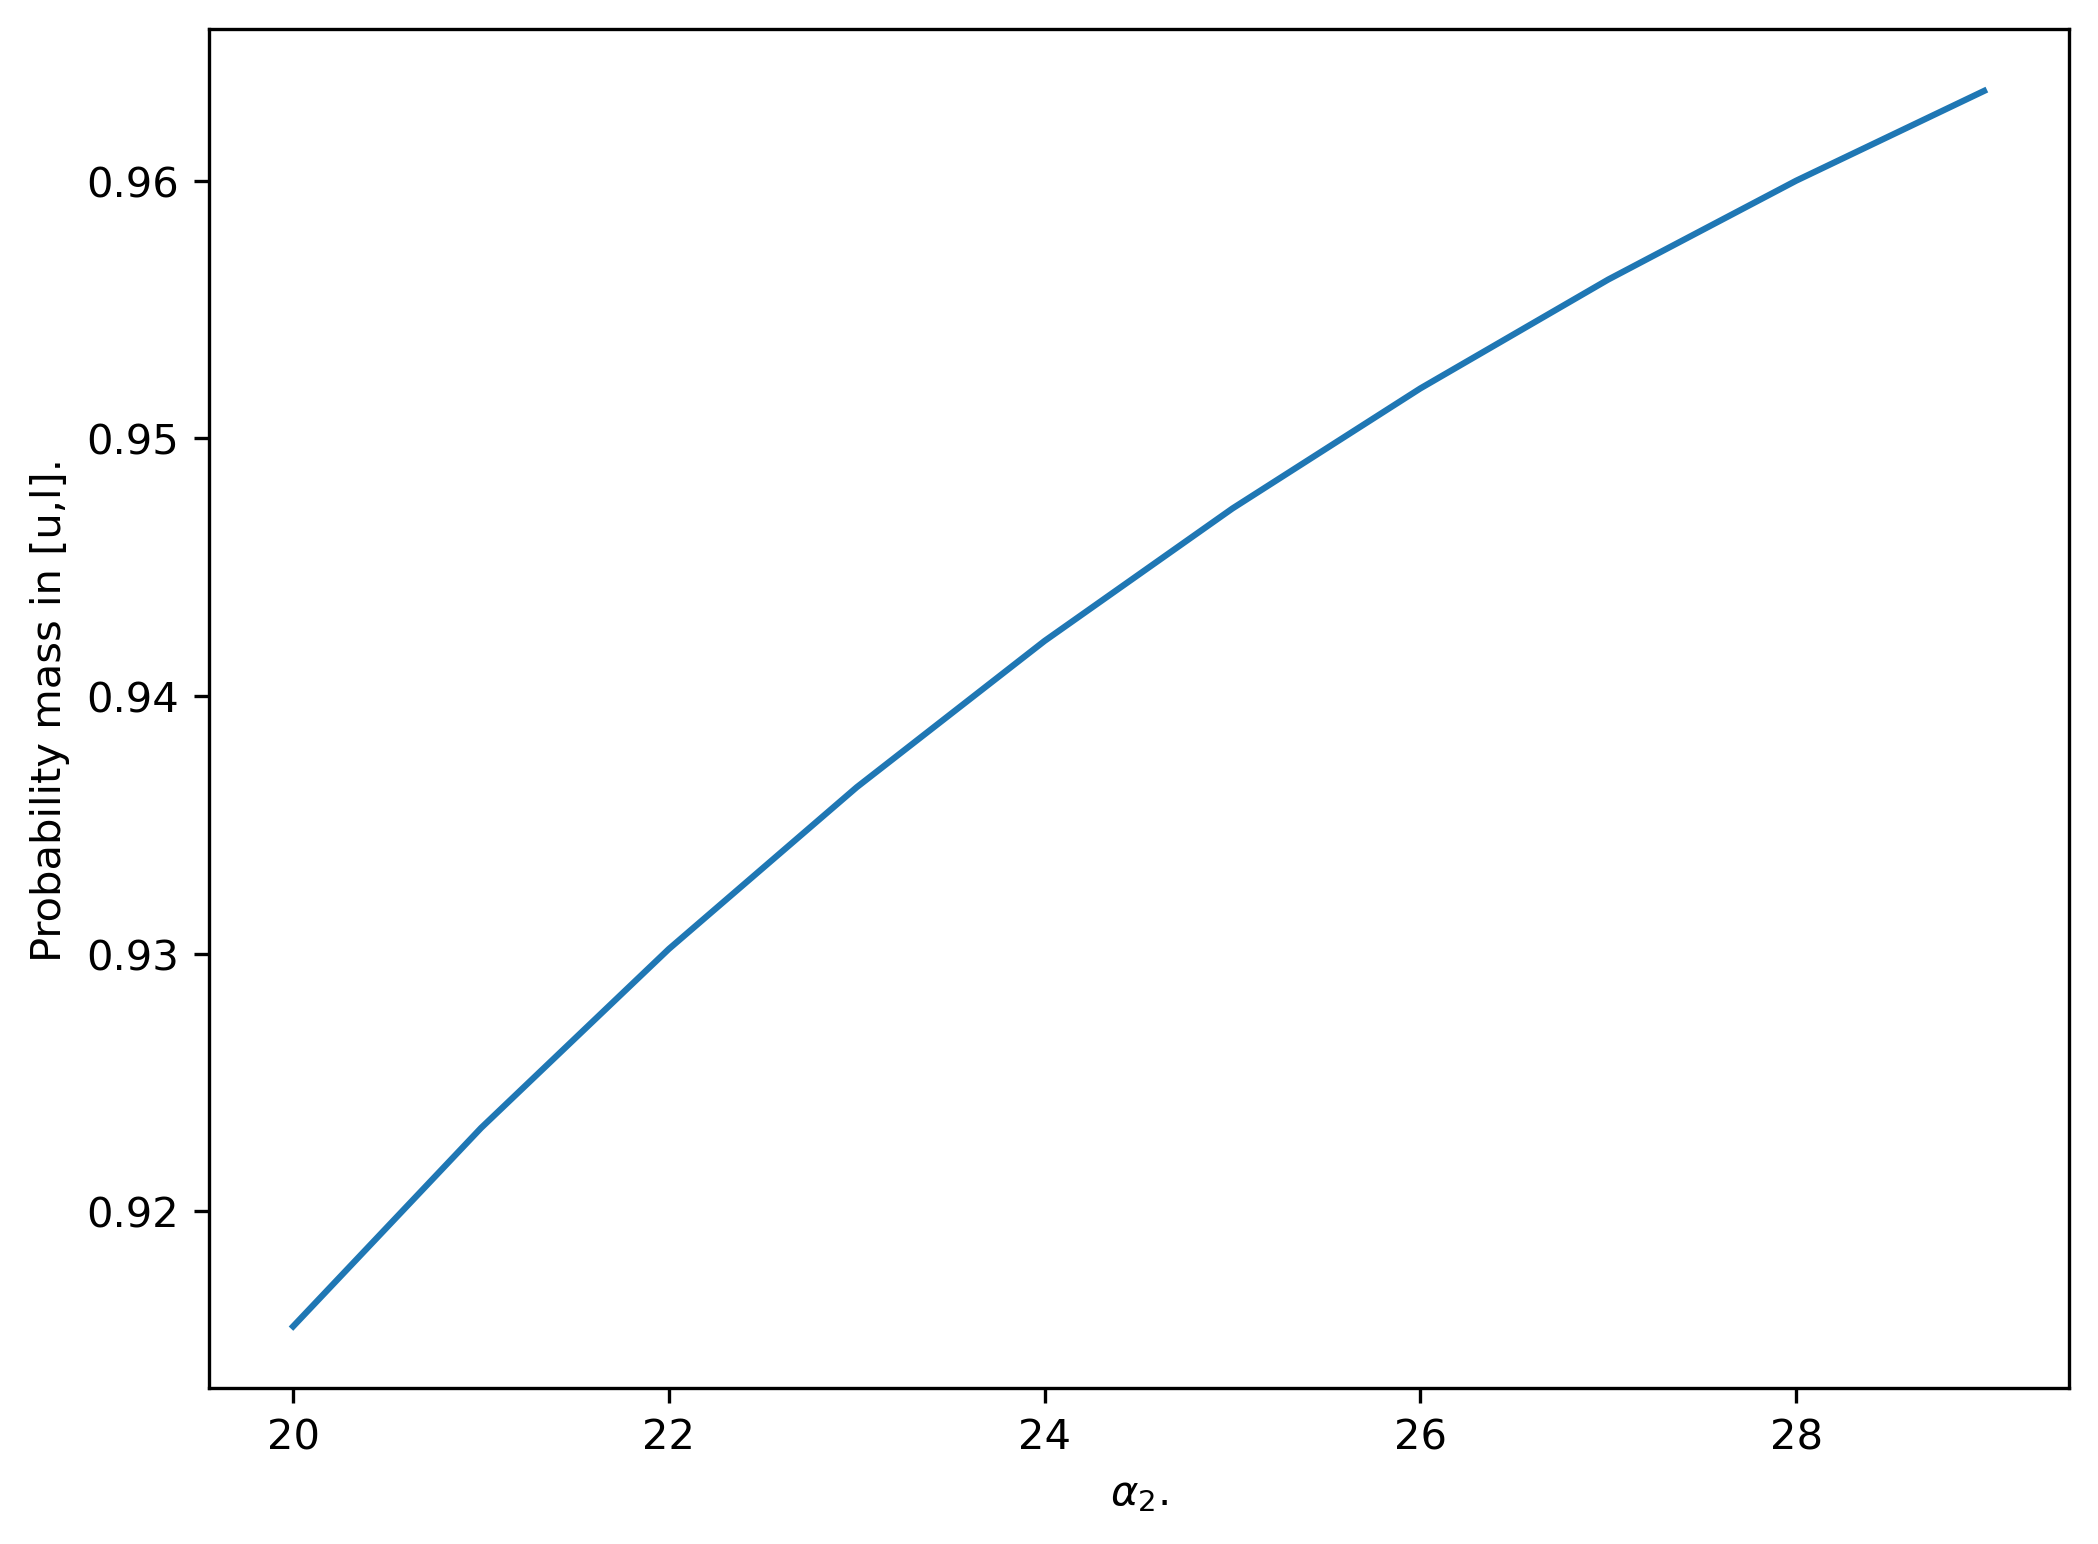
\includegraphics[width=7cm,height=5cm]{./figures/3-16.png}
\caption{Exercise 3.16.}
\end{figure}
So the optimal choice is $\alpha=26$.
This is tantamount to adopt 32 extra samples.

\subsection{Marginal likelihood for beta-binomial under uniform prior}
The marginal likelihood is given by:
$$p(N_{1}|N)=\int_{0}^{1} p(N_{1},\theta|N) \text{d}\theta = \int_{0}^{1} p(N_{1}|\theta,N)\cdot p(\theta)\text{d}\theta.$$

Plug in:
$$p(N_{1}|\theta,N)=\text{Bin}(N_{1}|\theta,N),$$
$$p(\theta) = \text{Beta}(\theta|1,1).$$

Thus:
\begin{align}
p(N_{1}|N)=&\int_{0}^{1} \binom{N}{N_{1}}\cdot \theta^{N_{1}}\cdot (1-\theta)^{N-N_{1}} \text{d}\theta \nonumber \\
=&\binom{N}{N_{1}}\cdot B(N_{1} +1,N-N_{1}+1)\nonumber \\
=&\frac{N!}{N_{1}!\cdot (N-N_{1})!}\cdot\frac{N_{1}! \cdot(N-N_{1})!}{(N+1)!}\nonumber \\
=&\frac{1}{N+1}. \nonumber
\end{align}

Where $B$ is the regulizer for a Beta distribution:
$$B(a,b)=\frac{\Gamma(a)\cdot\Gamma(b)}{\Gamma(a+b)}.$$

The physics behind this setting is that if no prior information is introduced then all $N+1$ possibilities are equal likely to appear.

\subsection{Bayes factor for coin tossing}
The Bayes factor for hypothesis test is defined by:
$$\text{BF}_{1,0}=\frac{p(\text{data}|H_{1})}{p(\text{data}|H_{0})},$$
where $H_{0}$ is the null hypothesis.

We have:
$$p(\text{data}|H_{0})=\text{Bin}(9|0.5,10)=\binom{10}{9}\cdot 0.5^{10}\approx 0.00977.$$
And
$$p(\text{data}|H_{1})=\frac{1}{10+1}\approx 0.09091,$$
according to Exercise 3.17.
The Bayes factor is approximately $9.3$.

When $N=100$ and $N_{1}=90$, the Bayes factor is:
$$\frac{\frac{1}{100+1}}{\binom{100}{90}\cdot 0.5^{100}}>\frac{2^{100}}{101^{11}}\approx 113622530.$$

When $\frac{N}{N_{1}}$ remains a constant deviated from 0.5, the larger $N$ is, the more likely that the coin is biased.
This is an intuitive conclusion from the law of large numbers.


\subsection{Irrelevant features with naive Bayes}
The log-likelihood is defined by:
$$\log p(\textbf{x}_{i}|c,\theta)=\sum_{w=1}^{W}x_{iw}\cdot \log \frac{\theta_{cw}}{1-\theta_{cw}}+\sum_{w=1}^{W}\log (1-\theta_{cw}).$$

In a succint way:
$$\log p(\textbf{x}_{i}|c,\theta)=\phi(\textbf{x}_{i})^{\text{T}} \beta_{c},$$
where:
$$\phi(\textbf{x}_{i})=(\textbf{x}_{i},1)^{\text{T}},$$
$$\beta_{c}=\left(\log \frac{\theta_{c1}}{1-\theta_{c1}},...\sum_{w=1}^{W}\log(1-\theta_{cw})\right)^{\text{T}}.$$

For question (a):
\begin{align}
\log \frac{p(c=1|\textbf{x}_{i})}{p(c=2|\textbf{x}_{i})} =&\log \frac{p(c=1)\cdot p(\textbf{x}_{i}|c=1)}{p(c=2)\cdot p(\textbf{x}_{i}|c=2)} \nonumber \\
=&\log \frac{p(\textbf{x}_{i}|c=1)}{p(\textbf{x}_{i}|c=2)} \nonumber \\
=&\phi(\textbf{x}_{i})^{\text{T}}(\beta_{1}-\beta_{2}). \nonumber
\end{align}

For question (b), with:
$$\log \frac{p(c=1|\textbf{x}_{i})}{p(c=2|\textbf{x}_{i})} = \log \frac{p(c=1)}{p(c=2)} +  \phi(\textbf{x}_{i})^{T}(\beta_{1}-\beta_{2}),$$
a word $w$ will not affect this posterior measure as long as:
$$x_{iw}(\beta_{1,w}-\beta_{2,w})=0$$

Hence if:
$$\theta_{c=1,w}=\theta_{c=2,w},$$
then it cannot affect the classification decision.
That is to say, $w$ appear in class 1 and 2 with the same frequency.

For question (c), we have:
$$\hat{\theta}_{1,w}=1-\frac{1}{2+N_{1}},$$
$$\hat{\theta}_{2,w}=1-\frac{1}{2+N_{2}}.$$
They are different when $N_{1} \neq N_{2}$ so the bias effect remains.
However, this bias reduces when $N$ grows large.

For question (d), using information theory would be a solid option.

\subsection{Class conditional densities for binary data}
For question (a), we have:
$$p(\textbf{x}|y=c)=\prod_{i=1}^{D}p(x_{i}|y=c,x_{1},...,x_{i-1}).$$
The number of parameter in this case is:
$$C\cdot \sum_{i=0}^{D-1}2^{i}=C\cdot(2^{D+1}-2) = \mathcal{O}(C\cdot 2^{D}).$$

For question (b) and (c), the overfitting is generally assmued to decline when $N$ grows.
The dependence within the variables generally hinder generalization when $N$ is small, but it could correctly capture the dependence, be it exist.

For question (d), fitting each parameter for the naive Bayes model requires averaging all components in the samples belong to one class, which is of complexity order $\mathcal{O}(N)$. The total complexity is thus of order $\mathcal{O}(C\cdot D\cdot N)$.
For the full Bayes classifier, the complexity is of order $\mathcal{O}(C\cdot 2^{D}\cdot N)$.

For question (e), the cost of inference in naive Bayes model is $\mathcal{O}(C\cdot D)$ for each sample.
While that for full Bayes model is $\mathcal{O}(C\cdot 2^{D})$.

For question (f), we have:
$$p(y|\textbf{x}_{v},\theta)\propto p(y|\theta)\cdot p(\textbf{x}_{v}|\theta)\propto\sum_{\textbf{x}_{h}}p(\textbf{x}_{v},\textbf{x}_{h}|\theta),$$
where we assumed a uniform prior on all classes since it is not the bottleneck of complexity.
The complexity for the naive model is then:
$$\mathcal{O}(C\cdot v\cdot 2^{h}),$$
while that for the full model is:
$$\mathcal{O}(C\cdot 2^{v})\cdot 2^{h}).$$


\subsection{Mutual information for naive Bayes classifiers with binary features}
By definition:
$$I(X;Y)=\sum_{x_{j}}\sum_{y}p(x_{j},y)\log \frac{p(x_{j},y)}{p(x_{j})\cdot p(y)}.$$
For binary features, the value of $x_{j}$ is either zero or one.
Given $\pi_{c}=p(y=c),\theta_{jc}=p(x_{j}=1|y=c),\theta_{j}=p(x_{j}=1)$, we have the mutual information between $x_{j}$ and $Y$ be:
\begin{align}
I_{j}=&\sum_{c}p(x_{j}=1,c)\log \frac{p(x_{j}=1,c)}{p(x_{j}=1)\cdot p(c)}\nonumber \\
 +& \sum_{c}p(x_{j}=0,c)\log \frac{p(x_{j}=0,c)}{p(x_{j}=0)\cdot p(c)} \nonumber \\
=&\sum_{c}\pi_{c}\theta_{jc} \log \frac{\theta_{jc}}{\theta_{j}} + (1-\theta_{jc})\pi_{c} \log \frac{1-\theta_{jc}}{1-\theta_{j}},\nonumber
\end{align}
which ends in (3.76).

\subsection{Fitting a naive Bayesian spam filter by hand}
$\theta_{\text{spam}}$ is $\frac{3}{3+4}$.

$\theta_{\text{secret}|\text{spam}}$ is $\frac{2}{3}$.

$\theta_{\text{secret}|\text{non-spam}}$ is $\frac{1}{4}$.

$\theta_{\text{sports}|\text{non-spam}}$ is $\frac{1}{2}$.

$\theta_{\text{dollar}|\text{spam}}$ is $\frac{1}{3}$.

\newpage
\section{Gaussian models}
Though being a family of models for continuous variables, traditional Gaussian models do not cast a more important role than models covered in the chapter before.
Since in most scenarios, the assumption that the data are subject to a normal distribution is unrealistic.

However, Gaussian models are crucial for latent space analysis.
Even for complex objects such as image or video, the assumption that they can be encoded into features under a Gaussian distribution turns out to be reliable.
Moreover, Gaussian models pave the way to general variational inference and Gaussian process, an important kernel machine.

For the reason above one cannot overestimate the significance of Gaussian models, be their history so long.
Most of the mathematical difficulties with Gaussian model have been covered in sections (marked with stars) in the textbook.

\subsection{Uncorrelated does not imply independent}
The mean for $Y$ is:
$$\int_{-1}^{1}X^{2}\text{d}X=\mathbb{E}[X^{2}].$$
Calculate the covariance of $X$ and $Y$:
\begin{align}
\text{cov}(X,Y)=&\int\int (X-\mathbb{E}(X))\cdot (Y-\mathbb{E}(Y))\cdot p(X,Y)\text{d}X\text{d}Y \nonumber \\
=&\int_{-1}^{1}X(X^{2}-\mathbb{E}[X^{2}])\text{d}X=0, \nonumber
\end{align}
whose value is zero since we are intergrating an odd function in range $[-1,1]$, hence:

$$\rho(X,Y)=\frac{\text{cov}(X,Y)}{\sqrt{\text{var}(X)\text{var}(Y)}}=0.$$

Independence is a much stronger condition than uncorrelation.
The former exerts constrains on the $\sigma$-algebra that random variables generates while the later only regulates the value of the expectation of a new random variable.
Decomposition $p(X,Y)=p(X)\cdot p(Y)$ is sufficient for reducing the covariance to zero, but not necessary.

\subsection{Uncorrelated and Gaussian does not imply independent unless jointly Gaussian}
For question (a).
The p.d.f. for $Y$ is:
$$p(Y\in[a,a+\text{d}a])=0.5 \cdot p(X\in[a,a+\text{d}a]) + 0.5 \cdot p(X\in[-a-\text{d}a],-a)=p(X\in[a,a+\text{d}a]),$$
since $X$ is symmetric.
So $Y$ subject to a normal distribution $(0,1)$.

For question (b), we have:
\begin{align}
\text{cov}(X,Y)=&\mathbb{E}(XY)-\mathbb{E}(X)-\mathbb{E}(Y) \nonumber \\
=& \mathbb{E}_{W}(\mathbb{E}(XY|W)) - 0 \nonumber \\
=&0.5\cdot\mathbb{E}(X^{2})+0.5\cdot\mathbb{E}(-X^{2})=0. \nonumber
\end{align}
So they are uncorrelated.

To disprove dependence (in case of confusion), let:
$$a=\Phi^{-1}(\frac{1}{4}),$$
where $\Phi$ is the c.d.f of $X$, i.e.:
$$\int_{-\infty}^{a}\mathcal{N}(x|0,1)\text{d}x=\frac{1}{4}.$$

Let $R_{1}=(-\infty,a]$, $R_{2}=(a,0]$.
The space of experiment results for $X\times Y$ is $\mathcal{R}^{2}$.
Let $R_{1}\times R_{2}$ be a Borel set in $\mathcal{R}^{2}$.
Be $X$ and $Y$ independent, its probability measure should be $\frac{1}{16}$.
However, when $X\in R_{1}$, it is impossible for $Y$ to take a value from $R_{2}$. Hence the independency fails.

The rule of iterated expectation is but the Bayes rule:
$$
\begin{aligned}
\mathbb{E}[XY]&=\int_{X}\int_{Y}XY\cdot p(X,Y)\text{d}X\text{d}Y\\
&=\int_{X}\int_{Y}XY\cdot \left(\int_{W} p(X,Y,W)\text{d}W\right)\text{d}X\text{d}Y\\
&=\int_{W}\left(\int_{X}\int_{Y} XY\cdot p(X,Y|W)    \right)p(W)\text{d}W.
\end{aligned}
$$

\subsection{Correlation coefficient is between -1 and 1}
With out loss of generality, assume $\mathbb{E}[X]=\mathbb{E}[Y]=0$.
The statement:
$$-1 \leq \rho(X,Y) \leq 1,$$
is equal to
$$|\rho(X,Y)| \leq 1.$$
Hence we are to prove:
$$|\text{cov}(X,Y)|^{2} \leq \text{var}(X)\cdot \text{var}(Y)$$

Which can be drawn straightforwardly from Cauchy–Schwarz inequality.
Let
$$g(t)=t^{2}\cdot\text{var}(X)+2t\cdot\text{var}(X,Y)+\text{var}{Y}=\mathbb{E}[(tX+Y)^{2}]\geq 0.$$
Taking $g$'s discriminator finishes the proof.

\subsection{Correlation coefficient for linearly related variables is 1 or -1}
When $Y=aX+b$:
$$\mathbb{E}(Y)=a\cdot\mathbb{E}(x)+b,$$
$$\text{var}(Y)=a^{2}\cdot \text{var}(X).$$

Therefore:
\begin{align}
cov(X,Y)=&\mathbb{E}(XY)-\mathbb{E}(X)\cdot\mathbb{E}(Y)\nonumber \\
=&a\cdot\mathbb{E}(X^{2})+b\cdot\mathbb{E}(X)-a\cdot\mathbb{E}^{2}(X)-b\cdot\mathbb{E}(X)\nonumber \\
=&a\cdot \text{var}(X) \nonumber.
\end{align}
Meanwhile:
$$\text{var}(X)\cdot \text{var}(Y) = a^{2}\cdot \text{var}(X).$$
These two are sufficient to derive:
$$\rho(X,Y) = \frac{a}{|a|}.$$

\subsection{Normalization constant for a multidimensional Gaussian}
Assume $\mu=\textbf{0}$ w.l.o.g.
If the covariance matrix already takes a diagonal form:
$$\Sigma=\begin{pmatrix}
\lambda_{1}^{-1} & \cdots\\
\cdots & \cdots \\
\cdots& \lambda_{d}^{-1}
\end{pmatrix},$$
then:
$$
\begin{aligned}
\int\exp\left(-\frac{1}{2}\textbf{x}^{\text{T}}\Sigma\textbf{x}\right)\text{d}\textbf{x}&=\int\exp\left(-\frac{1}{2}\left(\sum_{i=1}^{d}\frac{x_{i}^{2}}{\lambda_{i}} \right) \right)\text{d}\textbf{x} \\
&=\prod_{i=1}^{d}\int\exp\left(-\frac{x_{i}^{2}}{2\cdot\lambda_{i}} \right)\text{d}x_{i}\\
&=(2\pi\lambda_{i})^{-\frac{d}{2}}.
\end{aligned}
$$
Plugging in $|\Sigma|=\prod_{i=1}^{d}\lambda_{i}^{-1}$ yields the desired normalization constant.
In the second equation, using the distribution law (though somewhat intimidating).

For the general case, we begin by diagonalizing $\Sigma$ into:
$$\Sigma=U^{\text{T}}\Lambda U,$$
where $\Lambda$ is a diagonal matrix with components $\lambda_{1}^{-1}\cdots \lambda_{d}^{-1}$ and $U$ is a orthogonal matrix.
The integral now becomes:
$$\int\exp\left(-\frac{1}{2}\left(U\textbf{x}\right)^{\text{T}}\Lambda\left(U\textbf{x}\right) \right)\text{d}\textbf{x}.$$
Since $|U|=1$ uniformly, we can directly rewrite the integral into:
$$\int\exp\left(-\frac{1}{2}\textbf{u}^{\text{T}}\Lambda\textbf{u} \right)\text{d}\textbf{u}.$$
The rest is repeating the diagonal case.

\subsection{Bivariate Gaussian}
We have:
$$
\begin{aligned}
p(x_{1},x_{2})&=\frac{1}{2\pi\sqrt{|\Sigma|}}\cdot\exp\left(-\frac{1}{2}(\textbf{x}-\mu)^{\text{T}}\Sigma (\textbf{x}-\mu) \right)\\
&=\frac{1}{2\pi\sigma_{1}\sigma_{2}\sqrt{1-\rho^{2}}}\cdot \exp\left(-\frac{1}{2}\begin{pmatrix}
x_{1}-\mu_{1} & x_{2}-\mu_{2}
\end{pmatrix}
\begin{pmatrix}
\sigma^{2}_{1} & \rho\sigma_{1}\sigma_{2} \\
\rho\sigma_{1}\sigma_{2} & \sigma^{2}_{2} \\
\end{pmatrix}
\begin{pmatrix}
x_{1}-\mu_{1} \\
 x_{2}-\mu_{2}
\end{pmatrix}
 \right).
\end{aligned}
$$

\subsection{Conditioning a bivariate Gaussian}
For question (a), we begin with the form from Exercise 4.6.:
$$p(x_{1},x_{2})=\frac{\exp\left(-\frac{1}{2(1-\rho^{2})}\left(\frac{(x_{1}-\mu_{1})^{2}}{\sigma^{2}_{1}}+\frac{(x_{2}-\mu_{2})^{2}}{\sigma^{2}_{2}}-2\rho\frac{(x_{1}-\mu_{1})(x_{2}-\mu_{2})}{\sigma_{1}\sigma_{2}} \right) \right)}{2\pi\sigma_{1}\sigma_{2}\sqrt{1-\rho^{2}}}.$$
By the Bayes rule:
$$p(x_{2}|x_{1})=\frac{p(x_{1},x_{2})}{p(x_{1})}.$$
So we only need to compute:
$$p(x_{1})=\int p(x_{1},x_{2}) \text{d}x_{2}.$$
This can be done by \emph{completing the square} inside $p(x_{1},x_{2})$ w.r.t. $x_{2}$:
$$
\begin{aligned}
2\pi\sigma_{1}\sigma_{2}\sqrt{1-\rho^{2}}\cdot p(x_{1},x_{2})&=\exp\left(-\frac{1}{2(1-\rho^{2})}\frac{(x_{1}-\mu_{1})^{2}}{\sigma^{2}_{1}} \right)\\
\cdot\exp&\left(-\frac{1}{2(1-\rho^{2})}\left(\frac{(x_{2}-\mu_{2})^{2}}{\sigma^{2}_{2}}-2\rho\frac{(x_{1}-\mu_{1})(x_{2}-\mu_{2})}{\sigma_{1}\sigma_{2}}+\frac{\rho^{2}(x_{1}-\mu_{1})^{2}}{\sigma^{2}_{1}} \right) \right)\\
&\cdot \exp\left(\frac{1}{2(1-\rho^{2})}\frac{\rho^{2}(x_{1}-\mu_{1})^{2}}{\sigma_{1}^{2}} \right)\\
&=\exp\left( -\frac{(x_{1}-\mu_{1})^{2}}{2\sigma^{2}_{1}}\right)\\
&\cdot \exp\left(-\frac{1}{2\sigma_{2}^{2}(1-\rho^{2})}\left((x_{2}-\mu_{2})-\frac{\sigma_{2}\rho(x_{1}-\mu_{1})}{\sigma_{1}} \right)^{2} \right).
\end{aligned}
$$
Now we are ready to perform the integrating:
$$
\begin{aligned}
\int p(x_{1},x_{2})\text{d}x_{2}&=\frac{\exp\left(-\frac{(x_{1}-\mu_{1})^{2}}{2\sigma^{2}_{1}} \right)}{2\pi\sigma_{1}\sigma_{2}\sqrt{1-\rho^{2}}}\cdot\int \exp\left(-\frac{1}{2 \sigma^{2}}(x_{2}-\mu)^{2} \right)\text{d}x_{2} \\
&=\frac{\exp\left(-\frac{(x_{1}-\mu_{1})^{2}}{2\sigma^{2}_{1}} \right)}{2\pi\sigma_{1}\sigma_{2}\sqrt{1-\rho^{2}}}\cdot \sqrt{2\pi\sigma^{2}_{2}(1-\rho^{2})},
\end{aligned}
$$
where
$$\sigma^{2}=\sigma^{2}_{2}(1-\rho^{2}),$$
$$\mu=\mu_{2}+\frac{\sigma_{2}\rho(x_{1}-\mu_{1})}{\sigma_{1}}.$$
Finally,
$$p(x_{2}|x_{1})=\frac{\exp\left(\frac{(x_{1}-\mu_{1})^{2}}{2\sigma^{1}}\right)\cdot \exp\left(-\frac{1}{2(1-\rho^{2})}\left(\frac{(x_{1}-\mu_{1})^{2}}{\sigma^{2}_{1}}+\frac{(x_{2}-\mu_{2})^{2}}{\sigma^{2}_{2}}-2\rho\frac{(x_{1}-\mu_{1})(x_{2}-\mu_{2})}{\sigma_{1}\sigma_{2}} \right) \right)}{\sqrt{2\pi\sigma^{2}_{2}(1-\rho^{2})}}.$$

For question (b), we can further simplify the numerator of $p(x_{2}|x_{1})$ into:
$$p(x_{2}|x_{1})=\frac{\exp\left(-\frac{1}{2(1-\rho^{2})}\left(\rho(x_{1}-\mu_{1})-(x_{2}-\mu_{2}) \right)^{2} \right)}{\sqrt{2\pi(1-\rho^{2})}}.$$

\subsection{Whitening vs standardizing}
Standardizing is a gold standard step for complex data, e.g., the \texttt{batch normalization} layer.
Whitening, although fancy, is harder to carry out since it involves solving an eigen problem.

\subsection{Sensor fusion with known variances in 1d}
Denate the two observed datasets by $Y^{(1)}$ and $Y^{(2)}$, with size $N_{1},N_{2}$, the likelihood is:
\begin{align}
p(Y^{(1)},Y^{(2)}|\mu)=&\prod_{n_{1}=1}^{N_{1}}p(Y^{(1)}_{n_{1}}|\mu)\cdot\prod_{n_{2}=1}^{N_{2}}p(Y^{(2)}_{n_{2}}|\mu)\nonumber \\
\propto& \exp\left\{ A\cdot \mu^{2} + B \cdot \mu \right\}, \nonumber
\end{align}
where we have dropped terms independent from $\mu$ and used:
\begin{align}
A=&-\frac{N_{1}}{2v_{1}}-\frac{N_{2}}{2v_{2}},\nonumber \\
B=&\frac{1}{v_{1}}\sum_{n_{1}=1}^{N_{1}}Y^{(1)}_{n_{1}} + \frac{1}{v_{2}}\sum_{n_{2}=1}^{N_{2}}Y^{(2)}_{n_{2}}. \nonumber
\end{align}
Differentiate the likelihood w.r.t. $\mu$ and set it to zero, we have:
$$\mu_{\text{MLE}} = -\frac{B}{2A}$$

The conjugate prior of this model must have a form proportional to $\exp\left\{A\cdot\mu^{2} + B\cdot\mu\right\}$, so it is a normal distribution:
$$p(\mu|a,b) \propto \exp\left\{ a\cdot \mu^{2} + b\cdot \mu \right\}.$$
The posterior distribution is:
$$p(\mu|Y) \propto \exp\left\{ (A+a)\cdot \mu^{2} + (B+b)\cdot \mu \right\}.$$
Hence we have the MAP estimation:
$$\mu_{\text{MAP}} = -\frac{B+b}{2(A+a)}.$$

It is noticable that the MAP converges to ML estimation when observation times grow:
$$\mu_{\text{MAP}} \rightarrow \mu_{\text{ML}}.$$
The posterior distribution is another normal distribution, with:
$$\sigma^{2}_{\text{MAP}} = -\frac{1}{2(A+a)}.$$

For non-informative prior, we have $a=b=0$ so $p(\mu|a,b)$ is uniform in the domain, then the MAP estimation is the same as MLE.

\subsection{Derivation of information form formulae for marginalizing and conditioning}
Plugging (4.93) and (4.95) into proven lines of (4.69) yields the information form formulae.

\subsection{Derivation of the NIW posterior}
We begin with the likelihood for a MVN:
$$p(\textbf{X}|\mu,\Sigma) = (2\pi)^{-\frac{ND}{2}}|\Sigma|^{-\frac{N}{2}}\exp\left\{ -\frac{1}{2}\sum_{n=1}^{N}(\textbf{x}_{i}-\mu)^{\text{T}}\Sigma^{-1}(\textbf{x}_{i}-\mu) \right\}.$$
By (4.195), which can be proven by:
\begin{align}
\sum_{n=1}^{N}(\textbf{x}_{i}-\mu)^{\text{T}}\Sigma^{-1}(\textbf{x}_{i}-\mu) =&\sum_{n=1}^{N}(\bar{\textbf{x}} - \mu + (\textbf{x}_{i} - \bar{\textbf{x}}))^{\text{T}}\Sigma^{-1}(\bar{\textbf{x}} - \mu + (\textbf{x}_{i} - \bar{\textbf{x}})) \nonumber \\
=&N(\bar{\textbf{x}}-\mu)^{\text{T}}\Sigma^{-1}(\bar{\textbf{x}}-\mu) + \sum_{n=1}^{N}(\textbf{x}_{i} - \bar{\textbf{x}})^{\text{T}}\Sigma^{-1}(\textbf{x}_{i}-\bar{\textbf{x}}) \nonumber \\
=&N(\bar{\textbf{x}}-\mu)^{\text{T}}\Sigma^{-1}(\bar{\textbf{x}}-\mu) + \text{tr}\left\{\Sigma^{-1}\sum_{n=1}^{N}(\textbf{x}_{i}-\bar{\textbf{x}})(\textbf{x}_{i} - \bar{\textbf{x}})^{\text{T}}\right\}\nonumber \\
=&N(\bar{\textbf{x}}-\mu)^{\text{T}}\Sigma^{-1}(\bar{\textbf{x}}-\mu) + \text{tr}\left\{ \Sigma^{-1} \textbf{S}_{\bar{\textbf{x}}}\right\},\nonumber
\end{align}
where we have used the fact that $\text{tr}(\textbf{Y}^{\text{T}}\textbf{Z})=\text{tr}(\textbf{Z}\textbf{Y}^{\text{T}})$, with $\textbf{Y}$ the shifted design matrix and $\textbf{Z}=\Sigma^{-1}\textbf{Y}$.

The conjugate prior for MVN's parameters $(\mu,\Sigma)$ is Normal-inverse-Wishart(NIW) distribution defined by:
$$\text{NIW}(\mu,\Sigma|\textbf{m}_{0},k_{0},v_{0},\textbf{S}_{0}) = \mathcal{N}(\mu|\textbf{m}_{0},\frac{1}{k_{0}}\Sigma)\cdot \text{IW}(\Sigma|\textbf{S}_{0},v_{0})$$
$$=\frac{1}{Z} |\Sigma|^{-\frac{v_{0} + D + 2}{2}}\cdot\exp\left\{ -\frac{k_{0}}{2}(\mu-\textbf{m}_{0})^{\text{T}}\Sigma^{-1}(\mu-\textbf{m}_{0})-\frac{1}{2}\text{tr}\left\{ \Sigma^{-1}\textbf{S}_{0} \right\} \right\}.$$
Hence the posterior reads (where we have omitted the condition on hyperparameters):
$$p(\mu,\Sigma|\textbf{X}) \propto |\Sigma|^{-\frac{v_{\textbf{X}}+D+2}{2}}\exp\left\{ -\frac{k_{\textbf{X}}}{2}(\mu-\textbf{m}_{\textbf{X}})^{\text{T}}\Sigma^{-1}(\mu-\textbf{m}_{\textbf{X}}) - \frac{1}{2}\text{tr}\left\{  \Sigma^{-1} \textbf{S}_{\textbf{X}}\right\} \right\},$$
where $v_{\textbf{X}}$, $k_{\textbf{X}}$, $\textbf{m}_{\textbf{X}}$ and $\textbf{S}_{\textbf{X}}$ are variables whose values are to be decided.
Only terms that dependent on $\mu$ and $\Sigma$ can explicitly enter the terms on the r.h.s.

Firstly, by comparing the exponential for $|\Sigma|$, we have:
$$v_{\textbf{X}} = v_{0} + N.$$
Secondly, compare the coefficient for the term $\mu^{\text{T}}\Sigma^{-1}\mu$ inside the exponential and we have:
$$k_{\textbf{X}} = k_{0} + N.$$
Thirdly, check the coefficient for $\mu^{\text{T}}$ so we have:
$$N\Sigma^{-1}\bar{\textbf{x}}+k_{0}\Sigma^{-1}\textbf{m}_{0}=k_{\textbf{X}}\Sigma^{-1}\textbf{m}_{\textbf{X}},$$
therefore:
$$\textbf{m}_{\textbf{X}} = \frac{N\bar{\textbf{x}}+k_{0}\textbf{m}_{0}}{k_{\textbf{X}}}.$$
Finally, recall that for an arbitrary column vector $A$:
$$A^{\text{T}}\Sigma^{-1}A=\text{tr}(A^{\text{T}}\Sigma^{-1}A)=\text{tr}(\Sigma^{-1}AA^{\text{T}}).$$
The terms that solely dependent on $\Sigma^{-1}$ should equal to each other, so:
$$\text{tr}(\Sigma^{-1}(k_{0}\textbf{m}_{0}\textbf{m}_{0}^{\text{T}}+\textbf{S}_{0}))+\text{tr}(\Sigma^{-1}(N\bar{\textbf{x}}\bar{\textbf{x}}^{\text{T}}\textbf{S}_{\bar{\textbf{x}}}))=\text{tr}(\Sigma^{-1}(k_{\textbf{X}}\textbf{m}_{\textbf{X}}\textbf{m}_{\textbf{X}}^{\text{T}}+\textbf{S}_{\textbf{X}})).$$
Having arrived in:
$$N \bar{\textbf{x}} \bar{\textbf{x}}^{\text{T}} + \textbf{S}_{\bar{\textbf{X}}} + k_{0}\textbf{m}_{0}\textbf{m}_{0}^{\text{T}} + \textbf{S}_{0} = k_{\textbf{X}}\textbf{m}_{\textbf{X}}\textbf{m}_{\textbf{X}}^{\text{T}} + \textbf{S}_{\textbf{X}},$$
we obtain:
$$\textbf{S}_{\textbf{X}} = N \bar{\textbf{x}} \bar{\textbf{x}}^{\text{T}} + \textbf{S}_{\bar{\textbf{X}}} + k_{0}\textbf{m}_{0}\textbf{m}_{0}^{\text{T}} + \textbf{S}_{0} - k_{\textbf{X}}\textbf{m}_{\textbf{X}}\textbf{m}_{\textbf{X}}^{\text{T}}.$$
Recall the definition for mean we ends in (4.214) since:
$$\textbf{S}=\sum_{n=1}^{N}\textbf{x}_{i}\textbf{x}_{t}^{\text{T}} = \textbf{S}_{\bar{\textbf{X}}} + N \bar{\textbf{x}}\bar{\textbf{x}}^{\text{T}}.$$
This finishes proving that the posterior distribution for MVN takes the form: $\text{NIW}(\textbf{m}_{\textbf{X}},k_{\textbf{X}},v_{\textbf{X}},\textbf{S}_{\textbf{X}}).$

\subsection{BIC for Gaussians}
For question (a), recall that the maximum likelihood estimation for a MVN model is:
$$\mu_{\text{MLE}}=\frac{1}{N}\sum_{n=1}^{N}\textbf{x}_{n},$$
$$\Sigma_{\text{MLE}}=\frac{1}{N}\sum_{n=1}^{N}(\textbf{x}_{n}-\mu_{\text{MLE}})(\textbf{x}_{n}-\mu_{\text{MLE}})^{\text{T}}.$$
So the likelihood reads:
$$
\begin{aligned}
p(\mathcal{D}|\mu_{\text{MLE}},\Sigma_{\text{MLE}})&=\prod_{n=1}^{N}p(\textbf{x}_{n}|\mu_{\text{MLE}},\Sigma_{\text{MLE}})\\
&=\prod_{n=1}^{N}(2\pi)^{-\frac{D}{2}}\cdot |\Sigma_{\text{MLE}}|^{-\frac{1}{2}}\cdot\exp\left(-\frac{1}{2}(\textbf{x}_{n}-\mu_{\text{MLE}})^{\text{T}}\Sigma^{-1}_{\text{MLE}}(\textbf{x}_{n}-\mu_{\text{MLE}}) \right)\\
&=(2\pi)^{-\frac{ND}{2}}\cdot |\Sigma_{\text{MLE}}|^{-\frac{N}{2}}\cdot\exp\left(-\frac{1}{2}\sum_{n=1}^{N}(\textbf{x}_{n}-\mu_{\text{MLE}})^{\text{T}}\Sigma^{-1}_{\text{MLE}}(\textbf{x}_{n}-\mu_{\text{MLE}})   \right).
\end{aligned}
$$
Denote:
$$\textbf{Y}=\begin{pmatrix}
\textbf{x}_{1}-\mu_{\text{MLE}}& \cdots & \textbf{x}_{N}-\mu_{\text{MLE}} \\
\end{pmatrix},$$
then $\Sigma_{\text{MLE}}=\frac{1}{N}\textbf{Y}\textbf{Y}^{\text{T}}$, while the term in the exponential of the likelihood is:
$$-\frac{1}{2}\cdot\text{tr}(\textbf{Y}^{\text{T}}\Sigma^{-1}_{\text{MLE}}\textbf{Y})=-\frac{1}{2}\cdot\text{tr}(\Sigma^{-1}_{\text{MLE}}\textbf{Y}\textbf{Y}^{\text{T}})=-\frac{ND}{2}.$$
Thus the BIC is:
$$-\frac{ND}{2}\cdot\log(2\pi\text{e})-\frac{N}{2}\cdot\log|\Sigma_{\text{MLE}}|-\frac{D+\frac{D(D+1)}{2}}{2}\cdot\log N.$$

For question (b), the fitting of a diagonal MVN model is tantamount to fitting $D$ independent 1d Gaussian models simultaneously, thus the $d$-th diagnoal component of $\Sigma^{\text{d}}_{\text{MLE}}$ is:
$$\frac{1}{N}\sum_{n=1}^{N}\textbf{x}_{n,d}^{2},$$
where we have assumed $\textbf{x}=\textbf{0}$ w.l.o.g.
Thus the term inside the exponential of the likelihood remains $-\frac{ND}{2}$.
So the BIC in this case is:
$$-\frac{ND}{2}\cdot\log(2\pi\text{e})-\frac{N}{2}\cdot\log|\Sigma^{\text{d}}_{\text{MLE}}|-D\cdot\log N.$$

We observe that if all $D$ components are mutually independent, i.e., $\Sigma_{\text{MLE}}$ is diagonal then the BIC for diagonal MVN model is strictly larger than that for general MVN, hence the diagonal version is always preferred.
In cases there exists dependence among components, the BIC for general MVN is still not necessarily larger than that of disgonal MVN.
This is a reflection of the trade-off between complexity and generalization.

The Bayesian information criterion is an approximation of a model's evidence, $p(\mathcal{D})$.
Let us start from:
$$p(\mathcal{D})=\int p(\mathcal{D}|\theta)\cdot p(\theta)\text{d}\theta,$$
where $\theta$ is the collection of all parameters within the current model.
The trick here is to expand $\log p(\textbf{x}|\theta)$ as a function of $\theta$ and taking approximation to the second order at $\theta_{\text{MAP}}$ so the first order gradient vanishes:
$$\log p(\textbf{x}|\theta)\approx \log p(\textbf{x}|\theta_{0})-\frac{1}{2}(\theta-\theta_{0})^{\text{T}} \textbf{H}(\theta-\theta_{0}),$$
where $\textbf{H}$ is the Hessian matrix at $\log p(\textbf{x}|\theta_{0})$.
Thus we have:
$$p(\textbf{x}|\theta)\approx p(\textbf{x}|\theta_{0})\cdot\exp\left(-\frac{1}{2}(\theta-\theta_{0})^{\text{T}} \textbf{H}(\theta-\theta_{0}) \right).$$
We are now ready to perform the integral, with:
$$p(\mathcal{D}|\theta)=p(\textbf{x}|\theta_{0})^{N}\cdot\exp\left(-\frac{N}{2}(\theta-\theta_{0})^{\text{T}}\textbf{H}(\theta-\theta_{0}) \right),$$
conducting the integral on the neighbour of $\theta_{0}=\theta_{\text{MAP}}$:
$$
\begin{aligned}
\int p(\mathcal{D}|\theta)\cdot p(\theta)\text{d}\theta&\approx p(\mathcal{D}|\theta_{\text{MAP}})\cdot p(\theta_{\text{MAP}})\cdot \int \exp\left(-\frac{N}{2}(\theta-\theta_{\text{MAP}})^{\text{T}}\textbf{H}(\theta-\theta_{\text{MAP}}) \right)\text{d}\theta \\
&=p(\mathcal{D}|\theta_{\text{MAP}})\cdot p(\theta_{\text{MAP}})\cdot (2\pi)^{\frac{d}{2}}|N^{-1}\textbf{H}^{-1}|^{\frac{1}{2}}\\
&=p(\mathcal{D}|\theta_{\text{MAP}})\cdot p(\theta_{\text{MAP}})\cdot (2\pi)^{\frac{d}{2}}\cdot N^{-\frac{d}{2}}\cdot |\textbf{H}^{-1}|^{\frac{1}{2}},\\
\end{aligned}
$$
where $d$ is the number of components in $\theta$.
Taking the logarithm of both side of the evidence yields the BIC.
One can see how many compromises and assumptions have been applied in deriving an analytic form of the evidence, which is arguably the most complex variable for Bayesian analysis.

See also \emph{PRML}, Section 4.4.

\subsection{Gaussian posterior credible interval}
Assume the prior distribution for an 1d normal distribution:
$$p(\mu) = \mathcal{N}(\mu|\mu_{0},\sigma^{2}_{0} = 9).$$
And the likelihood is:
$$p(x) = \mathcal{N}(x|\mu,\sigma^{2}=4).$$
Having observed $n$ variables, we want that the probability measure of $\mu$'s posterior distribution is no less than 0.95 within an interval no longer than 1.
The posterior for $\mu$ is:
\begin{align}
p(\mu|D) \propto p(\mu)\cdot p(D|\mu) =& \mathcal{N}(\mu|\mu_{0},\sigma^{2}_{0})\cdot \prod_{i=1}^{n}\mathcal{N}(x_{n}|\mu,\sigma^{2})\nonumber \\
\propto& \exp\left\{-\frac{1}{2\sigma^{2}_{0}}(\mu-\mu_{0})^{2}  \right\}\cdot \prod_{i=1}^{n}\exp\left\{  -\frac{1}{2\sigma^{2}}(x_{i}-\mu)^{2}\right\}\nonumber \\
=&\exp\left\{ (-\frac{1}{2\sigma_{0}^{2}}-\frac{n}{2\sigma^{2}})\mu^{2} + ... \right\},\nonumber
\end{align}
where we have dropped the terms inrevelent with $\mu$.
The posterior variance of $\mu$ is determined by the coefficient of $\mu^{2}$ in the exponential of the posterior distribution:
$$\sigma^{2}_{\text{post}}=\frac{\sigma^{2}_{0}\sigma^{2}}{\sigma^{2}+n\sigma^{2}_{0}}.$$
Since 0.95 of the probability mass for a normal distribution lies within $-1.96\sigma$ and $1.96\sigma$, we have:
$$n \geq 611.$$

\subsection{MAP estimation for 1d Gaussians}
Assume that the variance for this distribution $\sigma^{2}$ is known, and the mean $\mu$ is subject to a normal distribution with mean $m$ and variance $s^{2}$. Similiar to the question before, the posterior takes the form:
$$p(\mu|X) \propto p(\mu)\cdot p(X|\mu).$$
So the posterior is another normal distribution, by comparing the coefficient for $\mu^{2}$ in the exponential:
$$-\frac{1}{2s^{2}}-\frac{N}{2\sigma^{2}},$$
and that for $\mu$:
$$\frac{m}{s^{2}}+\frac{\sum_{n=1}^{N}x_{n}}{\sigma^{2}},$$
we have the posterior mean and variance by completing the square:
$$\sigma^{2}_{\text{post}} = \frac{s^{2}\sigma^{2}}{\sigma^{2}+Ns^{2}},$$
$$\mu_{\text{post}} = (\frac{m}{s^{2}}+\frac{\sum_{n=1}^{N}x_{n}}{\sigma^{2}})\cdot \sigma^{2}_{\text{post}}.$$
This finishes question (a).

For question (b), we already knew that the MLE is:
$$\mu_{\text{MLE}}=\frac{\sum_{n=1}^{N}x_{n}}{N}.$$
As $N$ increases, we have:
$$
\begin{aligned}
\lim_{N\rightarrow\infty}\mu_{\text{post}}&=\lim_{N\rightarrow\infty} \frac{\frac{\sigma^{2}}{s^{2}}\cdot m+\sum_{n=1}^{N}x_{n}}{\frac{\sigma^{2}}{s^{2}}+N}\\
&=\frac{\sum_{n=1}^{N}x_{n}}{N}.
\end{aligned}
$$

For question (c), when $s^{2}\rightarrow\infty$, $\mu_{\text{post}}$ also converges to $\mu_{\text{MLE}}$ since $\frac{\sigma^{2}}{s^{2}}\rightarrow 0$.

For question (d), when $s^{2}\rightarrow 0$, then $\frac{\sigma^{2}}{s^{2}}\rightarrow \infty$ and $\mu_{\text{post}}$ converges to $m$.

Both (c) and (d) are very intuitive.
$s^{2}\rightarrow\infty$ means a non-informative prior has been introduced so MAP is the same as MLE.
$s^{2}\rightarrow 0$ means that the knowledge that $\mu$ is close to $m$ is very strong so that finite observations cannot modify this belief.

\subsection{Sequential(recursive) updating of covariance matrix}
For question (a), note that:
$$n\textbf{C}_{n+1}-(n-1)\textbf{C}_{n}=\sum_{i=1}^{n+1}(\textbf{x}_{i}-\textbf{m}_{n+1})(\textbf{x}_{i}-\textbf{m}_{n+1})^{\text{T}}-\sum_{i=1}^{n}(\textbf{x}_{i}-\textbf{m}_{n})(\textbf{x}_{i}-\textbf{m}_{n})^{\text{T}}.$$
Making use of:
$$\textbf{m}_{n+1}=\frac{n\textbf{m}_{n}+\textbf{x}_{n+1}}{n+1},$$
we have:
$$
\begin{aligned}
n\textbf{C}_{n+1}-(n-1)\textbf{C}_{n}&=\textbf{x}_{n+1}\textbf{x}_{n+1}^{\text{T}}-(n+1)\textbf{m}_{n+1}\textbf{m}_{n+1}^{\text{T}}+n\textbf{m}_{n}\textbf{m}_{n}^{\text{T}}\\
&=\frac{n}{n+1}(\textbf{x}_{n+1}-\textbf{m}_{n})(\textbf{x}_{n+1}-\textbf{m}_{n})^{\text{T}}.
\end{aligned}
$$

For question (b), the complexity is $\mathcal{O}(d^{2})$.

For question (c), plugging (4.281) directly into (4.279) yields (4.280).

For question (d), the complexity remains $\mathcal{O}(d^{2})$.

\subsection{Likelihood ratio for Gaussians}
Consider a classifier for two classes, the generative distribution for them are two normal distributions $p(x|y=C_{i})=\mathcal{N}(x|\mu_{i},\Sigma_{i})$, by the Bayes rule:
$$\log \frac{p(y=1|x)}{p(y=0|x)} = \log \frac{p(x|y=1)}{p(x|y=0)} + \log \frac{p(y=1)}{p(y=0)}.$$
The first term on r.h.s. is the ratio of likelihood probability.

When we have arbitrary covariance matrices:
$$\frac{p(x|y=1)}{p(x|y=0)} = \sqrt{\frac{|\Sigma_{0}|}{|\Sigma_{1}|}}\cdot\exp\left\{ -\frac{1}{2}(x-\mu_{1})^{\text{T}}\Sigma_{1}^{-1}(x-\mu_{1}) + \frac{1}{2}(x-\mu_{0})^{\text{T}}\Sigma_{0}^{-1}(x-\mu_{0}) \right\}.$$
As $\Sigma_{0},\Sigma_{1}$ are arbitrary matrices, this formulation cannot be reduced further:
$$\log \frac{p(x|y=1)}{p(x|y=0)}=\frac{1}{2}\log \frac{|\Sigma_{0}|}{|\Sigma_{1}|}-\frac{1}{2}(x-\mu_{1})^{\text{T}}\Sigma_{1}^{-1}(x-\mu_{1})+\frac{1}{2}(x-\mu_{0})^{\text{T}}\Sigma_{0}^{-1}(x-\mu_{0}).$$
Note that the decision boundary ($\log \frac{p(x|y=1)}{p(x|y=0)}=0$) is a quardratic surface in $D$-dimension space.

When both covariance matrixes are given by $\Sigma$:
$$
\frac{p(x|y=1)}{p(x|y=0)} = \exp\left\{ -\frac{1}{2}(x-\mu_{1})^{\text{T}}\Sigma^{-1}(x-\mu_{1}) + \frac{1}{2}(x-\mu_{0})^{\text{T}}\Sigma^{-1}(x-\mu_{0}) \right\},
$$
so:
$$
\begin{aligned}
\log \frac{p(x|y=1)}{p(x|y=0)}&=-\frac{1}{2}(x-\mu_{1})^{\text{T}}\Sigma^{-1}(x-\mu_{1}) + \frac{1}{2}(x-\mu_{0})^{\text{T}}\Sigma^{-1}(x-\mu_{0})\\
&=\frac{1}{2}\text{tr}\left(\Sigma^{-1}\left[(x-\mu_{1})(x-\mu_{1})^{\text{T}}-(x-\mu_{2})(x-\mu_{2})^{\text{T}} \right] \right).
\end{aligned}
$$

When $\Sigma$ is a diagonal matrix, we have:
$$
\begin{aligned}
\log \frac{p(x|y=1)}{p(x|y=0)}&=-\frac{1}{2}(x-\mu_{1})^{\text{T}}\Sigma^{-1}(x-\mu_{1}) + \frac{1}{2}(x-\mu_{0})^{\text{T}}\Sigma^{-1}(x-\mu_{0})\\
&=\frac{1}{2}\text{tr}\left(\Sigma^{-1}\left[(x-\mu_{1})(x-\mu_{1})^{\text{T}}-(x-\mu_{2})(x-\mu_{2})^{\text{T}} \right] \right)\\
&=\frac{1}{2}\text{tr}\left(\Lambda^{-1} \Phi \right)\\
&=\frac{1}{2}\sum_{i=1}^{d}\lambda_{i}^{-1}\Phi_{i,i}.
\end{aligned}
$$
where:
$$\Phi=(x-\mu_{1})(x-\mu_{1})^{\text{T}}-(x-\mu_{2})(x-\mu_{2})^{\text{T}}.$$

Finally, if $\Sigma=\sigma^{2}I$ then:
$$
\log \frac{p(x|y=1)}{p(x|y=0)}=\frac{1}{2\sigma^{2}}\text{tr}(\Phi).
$$

Note that for the last three cases, the decision boundary is a linear plane in the space, since the quadratic term on $x$ has been cancelled in $\Phi$.

\subsection{LDA/QDA on height/weight data}
$\cdots$

\subsection{Naive Bayes with mixed features}
For question (a):
$$
\begin{aligned}
p(y=1|x_{1}=0,x_{2}=0)&=\frac{p(y=1)\cdot p(x_{1}|y=1)\cdot p(x_{2}=0|y=1)}{p(x_{1}=0,x_{2}=0)}\\
&=\frac{0.5\cdot 0.5 \cdot \frac{\exp(-0.5)}{\sqrt{2\pi}}}{p(x_{1}=0,x_{2}=0)}.
\end{aligned}
$$
Similarly,
$$p(y=2|x_{1}=0,x_{2}=0)=\frac{0.25*0.5*\frac{1}{\sqrt{2\pi}}}{p(x_{1}=0,x_{2}=0)},$$
$$p(y=3|x_{1}=0,x_{2}=0)=\frac{0.25*0.5*\frac{\exp(-0.5)}{\sqrt{2\pi}}}{p(x_{1}=0,x_{2}=0)}.$$
A normalization yields the final result by eliminating $p(x_{1}=0,x_{2}=0)$.

For question (b), we have:
$$p(y=1|x_{1}=0)=0.5,$$
$$p(y=2|x_{1}=0)=0.25,$$
$$p(y=3|x_{1}=0)=0.25,$$
since $x_{1}$ yields no more information for the classification label.

For question (c), we have:
$$p(y=1|x_{2}=0)\propto 0.5*\frac{\exp(-0.5)}{\sqrt{2\pi}},$$
$$p(y=2|x_{2}=0)\propto 0.25*\frac{1}{\sqrt{2\pi}},$$
$$p(y=3|x_{2}=0)\propto 0.25*\frac{\exp(-0.5)}{\sqrt{2\pi}}.$$
One can observe that unlike $p(y|x_{1}=0)$, $p(y|x_{1}=0)$ is different from the prior on labels.


\subsection{Decision boundary for LDA with semi tied covariances}
We begin from the Bayes rule:
$$p(y=1|\textbf{x},\theta) \propto p(y=1|\theta)\cdot p(\textbf{x}|y=1,\theta),$$
where we have omitted the terms independent of $y$.
With a uniform prior on two classes:
$$p(y=1|\textbf{x},\theta) \propto \mathcal{N}(\textbf{x}|\mu_{1},k\Sigma_{0}),$$
$$p(y=0|\textbf{x},\theta) \propto \mathcal{N}(\textbf{x}|\mu_{0},\Sigma_{0}).$$

The decision boundary, in which we are interested, is a curve depicted by $f(\textbf{x})=0$, where:
$$f(x)=\log \frac{p(y=1|\textbf{x},\theta)}{p(y=0|\textbf{x},\theta)}.$$
Therefore the decision boundary is:
$$\text{tr}\left(\Sigma^{-1}_{0}\left[\Phi(\textbf{x}) \right] \right)=d\cdot \ln k,$$
where:
$$\Phi(\textbf{x})=\frac{(\textbf{x}-\mu_{1})(\textbf{x}-\mu_{1})^{\text{T}}}{k}-(\textbf{x}-\mu_{0})(\textbf{x}-\mu_{0})^{\text{T}}.$$
The decision boundary is a quardratic curve unless $k=1$, which is geometrically very intuitive.

Let us consider a 2d case, focusing on the transformed coordinates where $\Sigma_{0}$ is the identity matrix.
With out loss of generality, let $\mu_{0}=(0,0)$, $\mu_{1}=(z,0)$, denote the distance between a point $p$ in this place from $\mu_{0}$ and $\mu_{1}$ by $a(p)$ and $b(p)$.
The decision boundary is exactly:
$$\left\{p:\frac{b(p)^{2}}{k}-a(p)^{2}=-\frac{1}{2}\ln k \right\}.$$
Plugging in the Cartesian representation $p(x,y)$, we ends up with a conical curve.
The linear transform of the space would not change its conical nature.

\subsection{Logistic regression vs LDA/QDA}
The underlying assumptions for all four classifiers are as follows:
\begin{itemize}
\item GaussI assumes a covariance matrix as identity matrix;
\item GaussX has not prior assumption on the covariance matrix;
\item LinLog assumes that different classes share the same covariance matrix;
\item QuadLog has not prior assumption on covariance matrix, yet it assumes that all data from one class are subject to a normal distribution;
\end{itemize}
From the perspective of complexity we have the following order:

QuadLog$=$GaussX$>$LinLog$>$GaussI.

The MLE likelihood should follow the same order, this answers question (a)-(d).

For question (e), the argument is untrue in general.
For example, model $M$ predicts two samples belonging to the first class with probability vectors $(0.49,0.51)$ and $(0.99,0.1)$.
While $M'$ outputs $(0.51,0.49)$ and $(0.51,0.49)$.
Now $M'$ is correct on both samples so $R(M)>R(M')$, but:
$$\frac{\log (0.49)+\log (0.99)}{2} > \frac{\log (0.51)+\log (0.51)}{2},$$
so $L(M)>L(M')$, this is sufficient for disproving the argument.

\subsection{Gaussian decision boundaries}
We have:
$$p(x|\mu_{i},\sigma^{2}_{i})=\frac{1}{\sqrt{2\pi\sigma^{2}_{i}}}\cdot\exp\left( -\frac{(x-\mu_{i}^{2})}{2\sigma^{2}_{i}}\right),$$
so:
$$p(x|\mu_{1},\sigma^{2}_{1})=\frac{1}{\sqrt{2\pi}}\cdot\exp\left(-\frac{x^{2}}{2} \right),$$
$$p(x|\mu_{2},\sigma^{2}_{2})=\frac{1}{10^{3}\cdot\sqrt{2\pi}}\cdot\exp\left(-\frac{(x-1)^{2}}{2\times 10^{6}} \right).$$
The decision region satisfies:
$$\frac{p(x|\mu_{1},\sigma^{2}_{1})}{p(x|\mu_{1},\sigma^{2}_{1})}\geq 1,$$
this is tantamount to:
$$\frac{(x-1)^{2}}{10^{6}}-x^{2}\geq -6\cdot \ln 10.$$
Denote $x_{1}$ and $x_{2}$ as the zeros of this quardratic form, then
$$R_{1}=[x_{1},x_{2}].$$

When $\sigma^{2}=\sigma^{1}$, $R_{1}$ is exactly $(\infty,\frac{1}{2})$.

One can solve for (a) and (b) by plugging in (4.289).

\subsection{QDA with 3 classes}
Solve (a) and (b) numerically:
\begin{lstlisting}[language=Python]
import math
import numpy as np
mu1=np.array([0,0])
mu2=np.array([1,1])
mu3=np.array([1,-1])
s1=np.array([[0.7,0],[0,0.7]])
s2=np.array([[0.8,0.2],[0.2,0.8]])
s3=np.array([[0.8,0.2],[0.2,0.8]])
def p(x):
    f1=np.linalg.det(s1)**(-0.5)*math.exp(-0.5*(mu1-x)@np.linalg.inv(s1)@(mu1-x))
    f2=np.linalg.det(s2)**(-0.5)*math.exp(-0.5*(mu2-x)@np.linalg.inv(s2)@(mu2-x))
    f3=np.linalg.det(s3)**(-0.5)*math.exp(-0.5*(mu3-x)@np.linalg.inv(s3)@(mu3-x))
    return f1,f2,f3
x1=np.array([-0.5,0.5])
x2=np.array([0.5,0.5])
print(p(x1))
print(p(x2))
\end{lstlisting}
The outcome is:
\begin{lstlisting}[language=Python]
(0.9995321962501862, 0.31309336105606445, 0.030361279346887253)
(0.9995321962501862, 1.005427487616282, 0.18990072283298057)
\end{lstlisting}
So the predicted labels are 1 and 2 respectively.


\subsection{Scalar QDA}
\begin{lstlisting}[language=Python]
import math
hm=[67,79,71]
hf=[68,67,60]
def mu(h):
    return (h[0]+h[1]+h[2])/3
def sigma2(h):
    m=mu(h)
    return ((h[0]-m)**2+(h[1]-m)**2+(h[2]-m)**2)/3
# For question (a):
mu_m=mu(hm)
mu_f=mu(hf)
sigma2_m=sigma2(hm)
sigma2_f=sigma2(hf)
print(mu_m)
print(sigma2_m)
print(mu_f)
print(sigma2_f)
# \pi_{m}=\pi_{f}=0.5.
# For question (b):
temp_m=(2*math.pi*sigma2_m)**(-0.5)*math.exp(-(72-mu_m)**2/2/sigma2_m)
temp_f=(2*math.pi*sigma2_f)**(-0.5)*math.exp(-(72-mu_f)**2/2/sigma2_f)
print(temp_m/(temp_m+temp_f))
\end{lstlisting}
For question (c) we can use a naive Bayes model, which is tantamount to adopting diagonal covariance matrices for both classes.


\newpage
\section{Bayesian statistics}
This Chapter is a continuation of Chapter 2.
Section 5.7.1.5. sheds light on PAC theory, the fundemantal theory underlying machine learning, elegant but somewhat impractical.
Section 5.7.3.1. introduces some basic elements from reinforcement learning.
Both branches requires solid and involved theories, especially those from probability.

\subsection{Proof that a mixture of conjugate priors is indeed conjugate}
The mixed conjugate prior takes the form (5.68):
$$p(\theta)=\sum_{k}p(z=k)\cdot p(\theta|z=k),$$
where $k$ is the index for mixed components.
Each $p(\theta|z=k)$ is a conjugate prior for the model, i.e., $p(\theta|z=k)$ and $p(\theta|z=k,\mathcal{D})$ takes the same form.

For the posterior in this case:
$$
\begin{aligned}
p(\theta|\mathcal{D})&=\sum_{k}p(\theta,z=k|\mathcal{D})\\
&=\sum_{k}p(z=k|\mathcal{D})\cdot p(\theta|z=k,\mathcal{D}).
\end{aligned}
$$
So the posterior is still a mixture of conjugate priors.
This is exactly (5.69), finally:
$$
\begin{aligned}
p(z=k|\mathcal{D})&= \frac{p(z=k,\mathcal{D})}{p(\mathcal{D})}\\
&=\frac{p(z=k)\cdot p(\mathcal{D}|p(z=k))}{\sum_{k'}p(z=k')\cdot p(\mathcal{D}|p(z=k'))},
\end{aligned}
$$
from Bayes rules.
The computation bottleneck in computing $p(z=k|\mathcal{D})$ is:
$$p(\mathcal{D}|z=k)=\int p(\mathcal{D}|\theta)\cdot p(\theta|z=k)\text{d}\theta,$$
which is not a easy task as well.


\subsection{Optimal threshold on classification probability}
For question (a), the posterior loss expectation for choosing action $\hat{y}$, given $x$, is:
$$
\begin{aligned}
\rho(\hat{y}|x)&=\mathbb{E}_{p(y|x)}[L(y,\hat{y})]\\
&=p_{0}\cdot L(\hat{y},0)+p_{1}\cdot L(\hat{y},1)\\
&=p_{0}\cdot  L(\hat{y},0)+(1-p_{0})\cdot L(\hat{y},1)\\
&=L(\hat{y},1)+p_{0}(L(\hat{y},0)-L(\hat{y},1)).
\end{aligned}
$$
Thus:
$$\rho(0|x)=\lambda_{01}-p_{0}\cdot \lambda_{01},$$
$$\rho(1|x)=p_{0}\cdot \lambda_{10}.$$
As both $\rho(0|x)$ and $\rho(1|x)$ are linear functions of $p_{0}$, hence the unique optimal threshold is where $\rho(0|x)=\rho(1|x)$, i.e.,
$$p_{0}=\frac{\lambda_{01}}{\lambda_{01}+\lambda_{10}},$$
$$p_{1}=\frac{\lambda_{10}}{\lambda_{01}+\lambda_{10}}.$$

For question (b), let $\lambda_{10}=1$, $\lambda_{01}=9$ will do.

\subsection{Reject option in classifiers}
For question (a), the posterior expected loss for choosing an non-reject action $\hat{y}$ given data $x$ is:
$$
\begin{aligned}
\rho(\hat{y}|x)&=\sum_{y=1}^{C} p(y|x)\cdot L(\hat{y},y)\\
&=\textbf{p}^{\text{T}}\textbf{l}(\hat{y}),
\end{aligned}
$$
where $\textbf{p}$ is the column vector encoding $p(y|x)$ and $\textbf{l}(\hat{y})$ is a column vector whose elements are $\lambda_{s}$ except for the $\hat{y}$-th one.
Thus the expected loss is $(1-p(\hat{y}|x))\cdot\lambda_{s}$ in this case, whose minimum is obtained by let
$$\hat{y}=\arg\max_{y}(p(y|x)).$$

For the reject option, the loss is uniformly $\lambda_{s}$.

Thus one should choose reject or $\hat{y}$ by minimizing:
$$\min (\lambda_{r},(1-p(\hat{y}|x))\cdot \lambda_{s}).$$

If
$$\lambda_{r}\leq (1-p(\hat{y}|x))\cdot\lambda_{s},$$
then we readily adopt the reject option.
This condition is tantamount to what is required to be prove:
$$p(\hat{y}|x)\leq 1-\frac{\lambda_{r}}{\lambda_{s}}.$$

For question (b), the minimum of the expected loss is:
$$\lambda_{s}\cdot \min\left\{\frac{\lambda_{r}}{\lambda_{s}},1-p(\hat{y}|x) \right\},$$
where $\hat{y}$ is the most probable class.
When $\frac{\lambda_{r}}{\lambda_{s}}$ is negligable, the reject option would always be chosen.
When $\frac{\lambda_{r}}{\lambda_{s}}$, the reject option would never be chosen.


\subsection{More reject options}
For question (a), we need to choose from:
$$(3,10\times (1-0.8)=2),$$
hence the optimal decision is class $0$.

For question (b), we need to choose from:
$$(3,10\times (1-0.6)=4),$$
hence the optimal decision is reject.

For question (c), the threshold is where:
$$\lambda_{r}=(1-p(\hat{y}|x))\cdot \lambda_{s}.$$
Plugging in figures we have:
$$p(\hat{y}|x)=0.7.$$
Thus $\theta_{1}=0.7$, $\theta_{0}=0.3$ by symmetry.

\subsection{Newsvendor problem}
We have:
$$\mathbb{E}(\pi|Q)=P\int_{0}^{Q}Df(D)\text{d}D-CQ\int_{0}^{Q}f(D)\text{d}D+(P-C)Q\int_{Q}^{+\infty}f(D)\text{d}D.$$
Taking derivative w.r.t. $Q$:
$$\frac{\partial}{\partial Q}\mathbb{E}(\pi|Q) = PQf(Q)-C\int_{0}^{Q}f(D)\text{d}D-CQf(Q)+(P-C)\int_{Q}^{+\infty}f(D)\text{d}D-(P-C)Qf(Q).$$
Setting  it to zero by making use of $\int_{0}^{Q}f(D)\text{d}D + \int_{Q}^{+\infty}f(D)\text{d}D=1$, we arrive in:
$$F(Q^{*})=\frac{P-C}{P},$$
where:
$$F(Q)=\int_{0}^{Q}f(D)\text{d}D$$
is the c.d.f. of $D$.

\subsection{Bayes factors and ROC curves}
If the prior on models are identical then both methods yields the same decision boundary.

\subsection{Bayes model averaging helps predictive accuracy}
Suppose the variable $\Delta$ is generated from a mixture of models, so:
$$p(\Delta|\mathcal{D})=\sum_{m\in\mathcal{M}}p(\Delta|m,\mathcal{D})\cdot p(m|\mathcal{D}).$$
The Bayes model averaging (BMA) result is just:
$$p^{\text{BMA}}(\Delta)=\sum_{m\in\mathcal{M}}p(\Delta|m,\mathcal{D})\cdot p(m|\mathcal{D}).$$
While that from an individual model $m\in \mathcal{M}$ is:
$$p^{m}(\Delta)=p(\Delta|m,\mathcal{D}).$$

The expected loss of the BMA result is:
$$\mathbb{E}_{p(\Delta)}[-\log p^{\text{BMA}}(\Delta)],$$
while that of model $m$ is:
$$\mathbb{E}_{p(\Delta)}[-\log p^{m}(\Delta)].$$
Now it is easy to see that:
$$\mathbb{E}_{p(\Delta)}[-\log p^{m}(\Delta)]-\mathbb{E}_{p(\Delta)}[-\log p^{\text{BMA}}(\Delta)]=\mathbb{KL}(p^{\text{BMA}}(\Delta)||p^{m}(\Delta)),$$
since the distribution on which the expectation is computed is just $p^{\text{BMA}}(\Delta)$.
Therefore the non-negativity of the KL divergence yields (5.127).

The conclusion from this exercise is of hardly any practical significance.
Since the underlying distribution is usually intractable, even with mixture Bayes model.
Once the form of the latent distribution is revealed, it is obvious that other distributions result in higher loss.

\subsection{MLE and model selection for a 2d discrete distribution}
For question (a), the joint distribution $p(x,y|\theta_{1},\theta_{2})$ is given by:
$$
\begin{aligned}
p(x=0,y=0)&=(1-\theta_{1})\cdot \theta_{2},\\
p(x=0,y=1)&=(1-\theta_{1})\cdot (1-\theta_{2}),\\
p(x=1,y=0)&=\theta_{1}\cdot (1-\theta_{2}),\\
p(x=1,y=1)&=\theta_{1}\cdot \theta_{2}.
\end{aligned}
$$
This can be compactly written as:
$$p(x,y|\theta_{1},\theta_{2})=\theta_{1}^{x}(1-\theta_{1})^{(1-x)}\theta_{2}^{x\odot y}(1-\theta_{2})^{(1-x\odot y)},$$
where $\odot$ is the Exclusive NOR operator.

For question (b), the MLE for $\theta_{1}$ is $\frac{4}{7}$, while that for $\theta_{2}$ is $\frac{4}{7}$.
Since we assumed the independency between $\theta_{1}$ and $\theta_{2}$, both MLE can be arrived at by simply counting.
The evidence is given by:
$$p(\mathcal{D}|\theta_{\text{MLE}})=\left(\frac{4}{7} \right)^{4}\cdot \left(\frac{3}{7} \right)^{3}\cdot \left(\frac{3}{7} \right)^{3} \cdot \left(\frac{4}{7} \right)^{4}.$$

For question (c), the MLE for $\theta$ is computed by normalizing the counting vector: $(2,1,2,2)$, so:
$$\theta_{\text{MLE}}=\left(\frac{2}{7},\frac{2}{7},\frac{1}{7},\frac{2}{7}\right).$$
The evidence is:
$$\left(\frac{2}{7} \right)^{2}\cdot \left(\frac{2}{7} \right)^{2}\cdot \left(\frac{1}{7} \right)\cdot \left(\frac{2}{7} \right)^{2}. $$

For question (d):
\begin{lstlisting}[language=Python]
import math
x=[1,1,0,1,1,0,0]
y=[1,0,0,0,1,0,1]
l2=0
l4=0
e=1/10**5
for shadow in range(7):
    temp1=0
    temp2=0
    temp00=0
    temp10=0
    temp01=0
    temp11=0
    for i in range(len(x)):
        if i==shadow:
            continue
        if x[i]==1:
            temp1=temp1+1
        if x[i]==y[i]:
            temp2=temp2+1
        if x[i]==0 and y[i]==0:
            temp00=temp00+1
        if x[i]==0 and y[i]==1:
            temp01=temp01+1
        if x[i]==1 and y[i]==0:
            temp10=temp10+1
        if x[i]==1 and y[i]==1:
            temp11=temp11+1
    theta_1=temp1/(len(x)-1)
    theta_2=temp2/(len(x)-1)
    s=temp00+temp01+temp10+temp11
    theta_00=temp00/s
    theta_01=temp01/s
    theta_10=temp10/s
    theta_11=temp11/s
    p2=theta_1**(x[shadow])*(1-theta_1)**(1-x[shadow])*theta_2**(1-x[shadow]^y[shadow])*(1-theta_2)**(x[shadow]^y[shadow])
    p4=theta_00**(x[shadow]==0 and y[shadow==0])*theta_01**(x[shadow]==0 and y[shadow==1])*theta_10**(x[shadow]==1 and y[shadow==0])*theta_11**(x[shadow]==1 and y[shadow==1])
    l2=l2+math.log(p2+e)
    l4=l4+math.log(p4+e)
print(l2)
print(l4)
\end{lstlisting}
The result is:
\begin{lstlisting}[language=Python]
-12.136441189337646
-28.04302596169576
\end{lstlisting}
Hence the CV will pick $M_{2}$.
The reason behind is that $M_{4}$ assumes zero probability for $(0,1)$ during the cross-validation, which significantly declines the confidence.

For question (e), the BIC for $M_{2}$ and $M_{4}$ are respectively:
$$\text{BIC}(M_{2},\mathcal{D})=-11.51,$$
$$\text{BIC}(M_{4},\mathcal{D})=-12.38.$$
Hence the BIC prefers $M_{2}$ as well.


\subsection{Posterior median is optimal estimate under L1 loss}
The posterior loss expectation is (where we have omitted $\mathcal{D}$ w.l.o.g.):
$$
\begin{aligned}
\rho(a) &= \int |y-a|p(y)\text{d}y = \int_{-\infty}^{a}(a-y)p(y)\text{d}y + \int_{a}^{+\infty}(y-a)p(y)\text{d}y\\
&=a\left\{\int_{-\infty}^{a}p(y)\text{d}y - \int_{a}^{+\infty}p(y)\text{d}y  \right\} -\int_{-\infty}^{a}yp(y)\text{d}y + \int_{a}^{+\infty}yp(y)\text{d}y.
\end{aligned}
$$
Differentiating the loss w.r.t. $a$ ends up with:
$$\frac{\partial}{\partial a}\rho(a) = \left\{\int_{-\infty}^{a}p(y)dy - \int_{a}^{+\infty}p(y)  \right\} + a\cdot 2p(a) - a\cdot 2p(a).$$
Set it to zero so:
$$\int_{-\infty}^{a}p(y)dy = \int_{a}^{+\infty}p(y),$$
whose summation is unity, hence $a$ satisfies:
$$\int_{-\infty}^{a}p(y)dy = \int_{a}^{+\infty}p(y)=\frac{1}{2},$$
which identifies the median.

\subsection{Decision rule for trading off FPs and FNs}
This is tantamount to exercise 5.2.
Replacing $\lambda_{01}$ by $c\cdot \lambda_{10}$, the rest follows the corresponding results.


\newpage
\section{Frequentist statistics}
For one who has delved into Bayesian statistics before acknowledging the frequentist statistics, the later is somewhat awkward and intimidating.
However, in most scenarios regarding science and engineering, the orthodox statistics remains the optimal candidate.
Since when the size of the dataset grows, the privilege of using Bayes is easily overwhelmed by the asymptotic performance of classical statistics.
Moreover, although Bayesians claim to have eliminated the overfitting problem with prior distributions, the subjectiveness in selecting hyperparameters also increases.
This problem cannot be solved with empirical Bayesian or more complex graphical structures, since none of them actually cut down the degree of freedom for parameters.

For the reasons above, the frequentist statistics should receive equal attention as, if not more than, the Bayesian version.

\subsection{Pessimism of LOOCV}
Under the setting in this problem, the best one classification method can achieve is an accuracy of 50\%, since the features are independent from the labels.
This is, however, the idealistic situation where we assume that $$N\rightarrow \infty,$$
where $N=N_{1}=N_{2}$.
When $N$ is finite, the classification accuracy usually fluctuate around 50\%.
In order for the label to be \emph{randomly} assigned, we should have that for an arbitrary (probabilistic) algorithm/machine that terminates within a time complexity a polynomial of $N_{i}$, its classification accuracy should not deviate from 50\% larger than $\frac{1}{p(N)}$, in which $p$ is an arbitrary polynomial function.
The machine in this case is refered to as probabilistic polynomial time (PPT) machine, and is of remarkable interest for cryptologists.
To generate cheap pseudo-random number efficiently is one of the most important task for cryptography.

For LOOCV, if a sample for class one is omitted, then the classification probability is:
$$(\frac{N-1}{2N-1},\frac{N}{2N-1}).$$
Hence the probability that the omitted sample is correctly labelled is:
$$\frac{N-1}{2N-1}\leq \frac{1}{2},$$
justifies its pessimism in this setting.

The dependency between features and labels paves the way of decoupling features or security/forensics in machine learning.
However, it is impossible to justifies that some dataset \emph{cannot be learned} by any machines, whose converse side is extremely simple.

\subsection{James Stein estimator for Gaussian means}
The prior for $\theta_{i}$ is:
$$\mathcal{N}(\theta_{i}|m_{0},\tau_{0}^{2}),$$
and the likelihood is given by:
$$\mathcal{N}(y_{i}|\theta_{i},\sigma^{2}).$$

For question (a), we begin by integrating out $\theta_{i}$ and establishing the dependency of $\mathcal{D}=\left\{y_{i} \right\}_{i=1}^{6}$ on $m_{0}$ and $\tau_{0}^{2}$:
$$
\begin{aligned}
p(y|m_{0},\tau_{0}^{2})&=\int p(y,\theta|m_{0},\tau_{0}^{2})\text{d}\theta \\
&=\int p(y|\theta\sigma^{2})\cdot p(\theta|m_{0},\tau_{0}^{2})\text{d}\theta \\
&= \frac{1}{2\pi\sqrt{\sigma^{2}\tau_{0}^{2}}}\cdot\int \exp\left\{-\frac{1}{2}\left( \frac{(y-\theta)^{2}}{\sigma^{2}}+\frac{(\theta-m_{0})^{2}}{\tau_{0}^{2}}\right) \right\}\text{d}\theta\\
&\propto\exp\left\{-\frac{1}{2}\left(-\frac{(\frac{y}{\sigma^{2}}+\frac{m_{0}}{\tau_{0}^{2}})^{2}}{\frac{1}{\sigma^{2}}+\frac{1}{\tau_{0}^{2}}}+\frac{y^{2}}{\sigma^{2}}\right) \right\} \int\exp\left\{(a\cdot\theta-b(y))^{2} \right\}\text{d}\theta\\
&\propto \exp\left\{-\frac{1}{2}\left( -\frac{(y+\frac{m_{0}\sigma^{2}}{\tau_{0}^{2}})^{2}}{\sigma^{2}+\frac{\sigma^{4}}{\tau_{0}^{2}}}+\frac{y^{2}}{\sigma^{2}} \right)\right\}\\
&=\mathcal{N}\left(y|m_{0},\sigma^{2}+\tau_{0}^{2}\right),
\end{aligned}
$$
where we have cancelled terms independent from $y$ and completing the square in the final step of deduction.
Given $\sigma^{2}=500$, we have:
$$\hat{m_{0}}=\bar{x}=1527.5,$$
$$\hat{\tau_{0}^{2}}=1878.58-\sigma^{2}=1378.58,$$

For question (b), the posterior distribution of $\theta_{i}$ given $y_{i}$ and other hyperparameters is:
$$
\begin{aligned}
p(\theta|y)&\propto p(\theta)\cdot p(y|\theta)\\
&\propto \exp\left\{-\frac{(\theta-m_{0})^{2}}{2\tau^{2}_{0}}-\frac{(\theta-y)^{2}}{2\sigma^{2}} \right\}\\
&=\mathcal{N}(\theta|\frac{m_{0}\sigma^{2}+y\tau_{0}^{2}}{\sigma^{2}+\tau_{0}^{2}},\frac{\sigma^{2}\tau_{0}^{2}}{\sigma^{2}+\tau_{0}^{2}}).
\end{aligned}
$$

For question (c), the interval is $(\mu'-1.96\sigma',\mu'+1.96\sigma')$, where $\mu'$ and $\sigma'$ are from question (b).

For question (d), a smaller $\sigma^{2}$ would reduce the ML-II into ordinary posterior analysis.
The parameter $\sigma^{2}$ can be understood as the \emph{noise} on the observations.
The less noise we assumed, the more precise the obsertvations are, and the intermedia $\theta$ becomes less necessary.

\subsection{$\hat{\sigma}^{2}_{\text{MLE}}$ is biased}
Consider:
$$\mathbb{E}[(x_{n}-\bar{x})^{2}]=\mathbb{E}[x_{n}^{2}]+\frac{1}{N^{2}}\sum_{j,k=1}^{N}\mathbb{E}[x_{j}x_{k}]-\frac{2}{N}\sum_{j=1}^{N}\mathbb{E}[x_{n}x_{j}].$$
The second term on the r.h.s. contains $N$ components that equal to $\mathbb{E}[x^{2}]=\mu^{2}+\sigma^{2}$ and $N^{2}-N$ components that equal to $\mathbb{E}[x_{l}x_{m}]=\mu^{2}$, where $l\neq m$.
For the third term, the numbers are $1$ and $N-1$, thus:
$$\mathbb{E}[(x_{n}-\bar{x})^{2}]=\frac{N-1}{N}\sigma^{2},$$
so is $\hat{\sigma}^{2}_{\text{MLE}}$.
The unbiased estimation, of which one who has taken several elementary courses on probability and statistics should have been very familiar, is:
$$\frac{N}{N-1}\cdot \hat{\sigma}^{2}_{\text{MLE}}.$$

\subsection{Estimation of $\sigma^{2}$ when $\mu$ is known}
The likelihood is:
$$p(x|\sigma^{2})=\frac{1}{\sqrt{2\pi\sigma^{2}}}\cdot\exp\left(-\frac{(x-\mu)^{2}}{2\sigma^{2}} \right).$$
Taking logarithm and gradient:
$$\frac{\text{d}}{\text{d}\sigma^{2}}\ln p(\mathcal{D}|\sigma^{2})=-\frac{N}{2\sigma^{2}}+\frac{1}{2\sigma^{4}}\sum_{n=1}^{N}(x_{n}-\mu)^{2}.$$
Setting it to zero yields:
$$\sigma_{\text{MLE}}^{2}=\frac{\sum_{n=1}^{N}(x_{n}-\mu)^{2}}{N}.$$

In this case the MLE is unbiased since:
$$\mathbb{E}(x_{n}-\mu^{2})=\mathbb{E}(x_{n}^{2})+\mu^{2}-2\mu\mathbb{E}(x_{n})=\sigma^{2}.$$




\newpage
\section{Linear regression}
\subsection{Behavior of training set error with increasing sample size}
The statement \textbf{the error on the test will always decrease as we get more training data, since the model will be better estimated} is not a gold standard.
The prerequisites behind this statement are at least:
\begin{itemize}
\item The test data shares the identical distribution with the training data.
Which, although plausible in general, fails in cases such as adversarial training (where an adversary schemes for samples that hinders the model) or defense against zero-day attack (where the model is required to detect an unknown threat from benign samples solely).
\item The model is complex enough to learn the knowledge embedded in the data.
For a basic example, a tabular predictor that only saves the latest finite samples and predicts by table looking-up.
In this case the size of the dataset would hardly help.
Moreover, the break of the i.i.d. assumption could worsen its performance.
\end{itemize}
We now reduce the discussion in cases where the assumptions for PAC learning holds.
When the training set is small, the trained model is usually over-fitted to the current data set (since the model is very complex), so the accuracy can be relatively high.
As the training set increases, the model has to learn to adapt to more general-purpose parameters, thus reducing the overfitting effect laterally, resulting in lower accuracy.
As pointed out in Section 7.5.4, increasing the training set is an important method of countering over-fitting besides adding regulizer.
In fact, increasing dataset is fundemantally the only solution to models' robustness, since one cannot exhaust all possible data augumentatin strategies.

\subsection{Multi-output linear regression}
For multi-output linear regression, if the outputs are independent, then for each output dimension subscripted by $j$, we have:
$$p(y_{j}|\textbf{x},\textbf{w}_{j})=\mathcal{N}(y_{j}|\textbf{x}^{\text{T}}\textbf{w}_{j},\sigma^{2}_{j}),$$
then:
$$p(\textbf{y}|\textbf{x},\textbf{W})=\prod_{j=1}^{M}\mathcal{N}(y_{j}|\textbf{x}^{\text{T}}\textbf{w}_{j},\sigma^{2}_{j}).$$
The independence implies:
$$p(\textbf{Y}|\textbf{X},\textbf{W})=\prod_{n=1}^{N}\prod_{j=1}^{M}\mathcal{N}(y_{n,j}|\textbf{x}_{n}^{\text{T}}\textbf{w}_{j},\sigma^{2}_{j}).$$
Taking its logarithm and saving terms dependent on $\textbf{W}$, we have:
$$\mathcal{L}(\textbf{W})=\sum_{n=1}^{N}\sum_{j=1}^{M}\frac{1}{\sigma^{2}_{j}}\left(y_{n,j}-\textbf{x}^{\text{T}}_{n}\textbf{w}_{j} \right)^{2}.$$
Interchanging the order of summation helps to decompose the loss into:
$$\sum_{j=1}^{M}\mathcal{L}_{j}(\textbf{w}_{j})=\sum_{j=1}^{M}\frac{1}{\sigma^{2}_{j}}\sum_{n=1}^{N}\left(y_{n,j}-\textbf{x}^{\text{T}}_{n}\textbf{w}_{j} \right)^{2},$$
where each:
$$\mathcal{L}_{j}(\textbf{w}_{j})=\frac{1}{\sigma^{2}_{j}}\sum_{n=1}^{N}\left(y_{n,j}-\textbf{x}^{\text{T}}_{n}\textbf{w}_{j} \right)^{2},$$
is but the MLE loss for a 1D linear regression.
Thus the columns of $\textbf{W}$ can be estimated independently by:
$$\textbf{w}_{j}^{\text{MLE}}=(\textbf{X}\textbf{X}^{\text{T}})^{-1}\textbf{X}\textbf{Y}_{j},$$
where $\textbf{X}$ is the $D*N$ design matrix and $\textbf{Y}$ is a columm matrix with length $N$ that embeds the $j$-th component of the output.
This is a little different from the symbols from the textbook but simple $\alpha$-reductions would elimiate such difference.
Equation (7.90) is incorrect by missing one design matrix.

As a compact way of writing $\textbf{W}^{\text{MLE}}$, we would have:
$$\textbf{W}^{\text{MLE}}=(\textbf{X}\textbf{X}^{\text{T}})^{-1}\textbf{X}\textbf{Y},$$
where $\textbf{Y}$ is a $N*M$ matrix.

For the case in this exercise, we have $D=2$, $N=6$, $M=2$:
$$\textbf{X}=
\begin{pmatrix}
1 & 1 & 1 & 0 & 0 & 0 \\
0 & 0 & 0 & 1 & 1 & 1
\end{pmatrix},$$
$$\textbf{Y}=
\begin{pmatrix}
-1 & -1 \\
-1 & -2 \\
-2 & -1 \\
1 & 1 \\
1 & 2 \\
2 & 1
\end{pmatrix}.$$
Thus:
$$\textbf{W}=\begin{pmatrix}
-\frac{4}{3} & -\frac{4}{3}\\
\frac{4}{3} & \frac{4}{3}
\end{pmatrix}.$$
One can observe that two columns for $\textbf{W}$ are identical, which is obvious by examing the two columns from $\textbf{Y}$.

\subsection{Centering and ridge regression}
The loss is given by:
$$\mathcal{L}(\textbf{w},w_{0})=\left(\textbf{y}-\textbf{X}^{\text{T}}\textbf{w}-w_{0}\textbf{1}\right)^{\text{T}}\left(\textbf{y}-\textbf{X}^{\text{T}}\textbf{w}-w_{0}\textbf{1}\right).$$

Taking partial gradient w.r.t. $w_{0}$ yields:
$$\frac{\partial}{\partial w_{0}} \mathcal{L}=\frac{\textbf{1}^{\text{T}}(\textbf{y}-\textbf{X}^{\text{T}}\textbf{w})}{N}.$$
Setting it to zero gives (7.94), where we have made use of $\bar{x}=0$.

Taking partial gradient w.r.t. $\textbf{w}$ yields:
$$\textbf{w}^{\text{MLE}}=(\textbf{X}\textbf{X}^{\text{T}}+\lambda \textbf{I})^{-1}\textbf{X}(\textbf{y}-w_{0}\textbf{1}).$$
In the equation (7.95), the observed data has to be centralized.

\subsection{MLE for $\sigma^{2}$ for linear regression}
The likelihood is given by:
\begin{align}
p(\mathcal{D}|\textbf{w},\sigma^{2})=&p(\textbf{Y}|\textbf{w},\sigma^{2},\textbf{X})\nonumber \\
=&\prod_{n=1}^{N}p(y_{n}|\textbf{x}_{n},\textbf{w},\sigma^{2})\nonumber \\
=&\prod_{n=1}^{N}\mathcal{N}(y_{n}|\textbf{w}^{\text{T}}\textbf{x}_{n},\sigma^{2})\nonumber \\
=&\frac{1}{(2\pi\sigma^{2})^{\frac{N}{2}}}\cdot\exp\left\{ -\frac{1}{2\sigma^{2}}\sum_{n=1}^{N}(y_{n}-\textbf{w}^{\text{T}}\textbf{x}_{n})^{2} \right\}.\nonumber
\end{align}
As for $\sigma^{2}$:
$$\frac{\partial}{\partial \sigma^{2}}\log p(\mathcal{D}|\textbf{w},\sigma^{2}) = -\frac{N}{2\sigma^{2}}+\frac{1}{2(\sigma^{2})^{2}}\sum_{n=1}^{N}(y_{n}-\textbf{w}^{\text{T}}\textbf{x}_{n})^{2}.$$
Setting it to zero yields:
$$\sigma^{2}_{\text{MLE}}=\frac{1}{N}\sum_{n=1}^{N}(y_{n}-\textbf{w}^{\text{T}}\textbf{x}_{n})^{2}.$$

\subsection{MLE for the offset term in linear regression}
For (7.97), we only have to use the second equation derived in exercise 7.3.

For (7.98), recall the third equation that we have derived in exercise 7.3.

\subsection{MLE for simple linear regression}
For (7.99), we plug the $D=1$ assumption into (7.98) so:
$$w_{1}^{\text{MLE}}=\frac{\sum_{n=1}^{N}(y_{n}-\bar{y})(x_{n}-\bar{x})}{\sum_{n=1}^{N}(x_{n}-\bar{x})^{2}}.$$
Recall that $\bar{x}=\frac{1}{N}\sum_{n=1}^{N}x_{n}$ and that for $\bar{y}$, so (7.99) is proven.

For (7.100), use (7.97) directly.

\subsection{Sufficient statistics for online linear regression}
For question (a), according to (7.99), $w_{1}$ can be estimated from $C_{xy}^{(n)}$ and $C_{xx}^{(n)}$ solely.

For question (b), according to (7.100), $w_{0}$ can be estimated from $\bar{x}^{(n)}$, $\bar{y}^{(n)}$ and $w_{1}$.
Hence $\bar{x}^{(n)}$, $\bar{y}^{(n)}$, $C_{xy}^{(n)}$ and $C_{xx}^{(n)}$ are necessary.

For question (c), the solution has been given by (7.103)-(7.104).
For $y$, the matter is simply an $\alpha$-reduction.

For question (d), we need to prove:
$$(n+1)C_{xy}^{(n+1)}=nC_{xy}^{(n)}+x_{n+1}y_{n+1}+n\bar{x}^{(n)}\bar{y}^{(n)}-(n+1)\bar{x}^{(n+1)}\bar{y}^{(n+1)}.$$
Expand the $C_{xy}$ in both two sides then the l.h.s. becomes:
$$\sum_{i=1}^{n+1}(x_{i}-\bar{x}^{(n+1)})(y_{i}-\bar{y}^{(n+1)}),$$
the r.h.s. becomes:
$$\sum_{i=1}^{n}(x_{i}-\bar{x}^{(n)})(y_{i}-\bar{y}^{(n)})+x_{n+1}y_{n+1}+n\bar{x}^{(n)}\bar{y}^{(n)}-(n+1)\bar{x}^{(n+1)}\bar{y}^{(n+1)}.$$
Finally, substituting the average at the $(n+1)$-th iteration in the l.h.s. and r.h.s. by (7.104), this is sufficient for arriving in (7.105).

For question (e) and (f):
\begin{lstlisting}[language=python]
import math
import matplotlib.pyplot as plt
x=[94,96,94,95,104,106,108,113,115,121,131]
y=[0.47,0.75,0.83,0.98,1.18,1.29,1.40,1.60,1.75,1.90,2.23]
bx=(x[0]+x[1])/2
by=(y[0]+y[1])/2
Cxx=((x[0]-bx)**2+(x[1]-bx)**2)/2
Cxy=((y[0]-by)*(x[0]-bx)+(y[1]-by)*(x[1]-bx))/2
w1=[]
w0=[]
for n in list(range(2,11)):
    bx_=bx+(x[n]-bx)/(n+1)
    by_=by+(y[n]-by)/(n+1)
    Cxx=(x[n]*x[n]+n*Cxx+n*bx*bx-(n+1)*bx_*bx_)/(n+1)
    Cxy=(x[n]*y[n]+n*Cxy+n*bx*by-(n+1)*bx_*by_)/(n+1)
    bx=bx_
    by=by_
    w1.append(Cxy/Cxx)
    w0.append(by-w1[n-2]*bx)
\end{lstlisting}
With:
\begin{figure}[htbp]
\centering
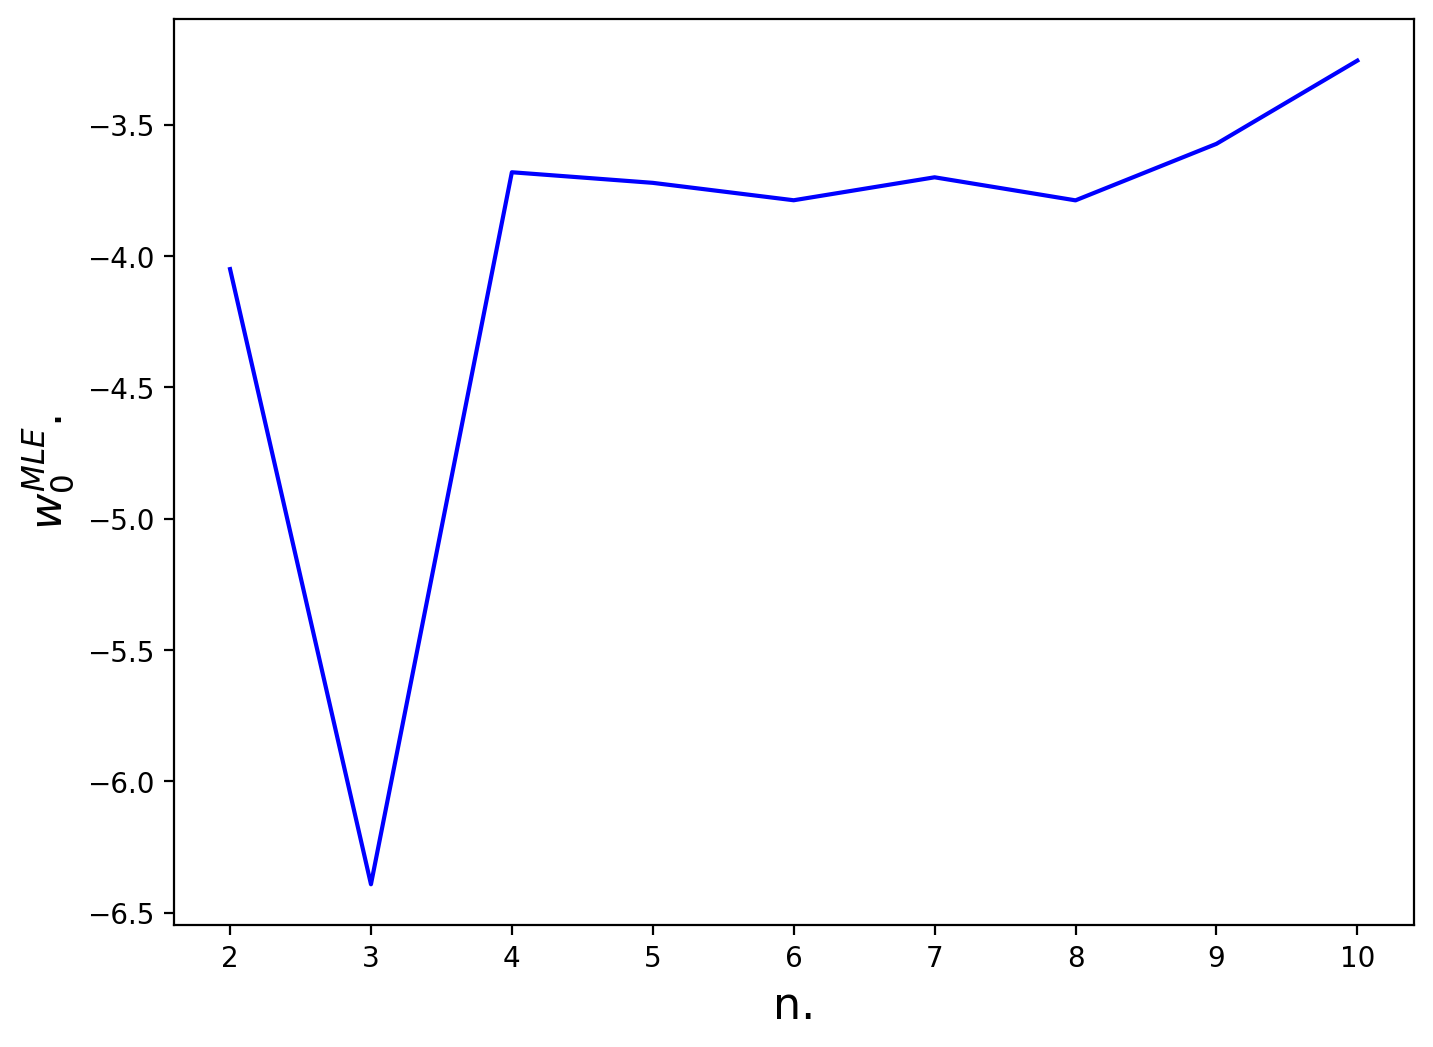
\includegraphics[width=7cm,height=5cm]{./figures/7-7-1.png}
\caption{Exercise 7.7. P1}
\end{figure}
\begin{figure}[htbp]
\centering
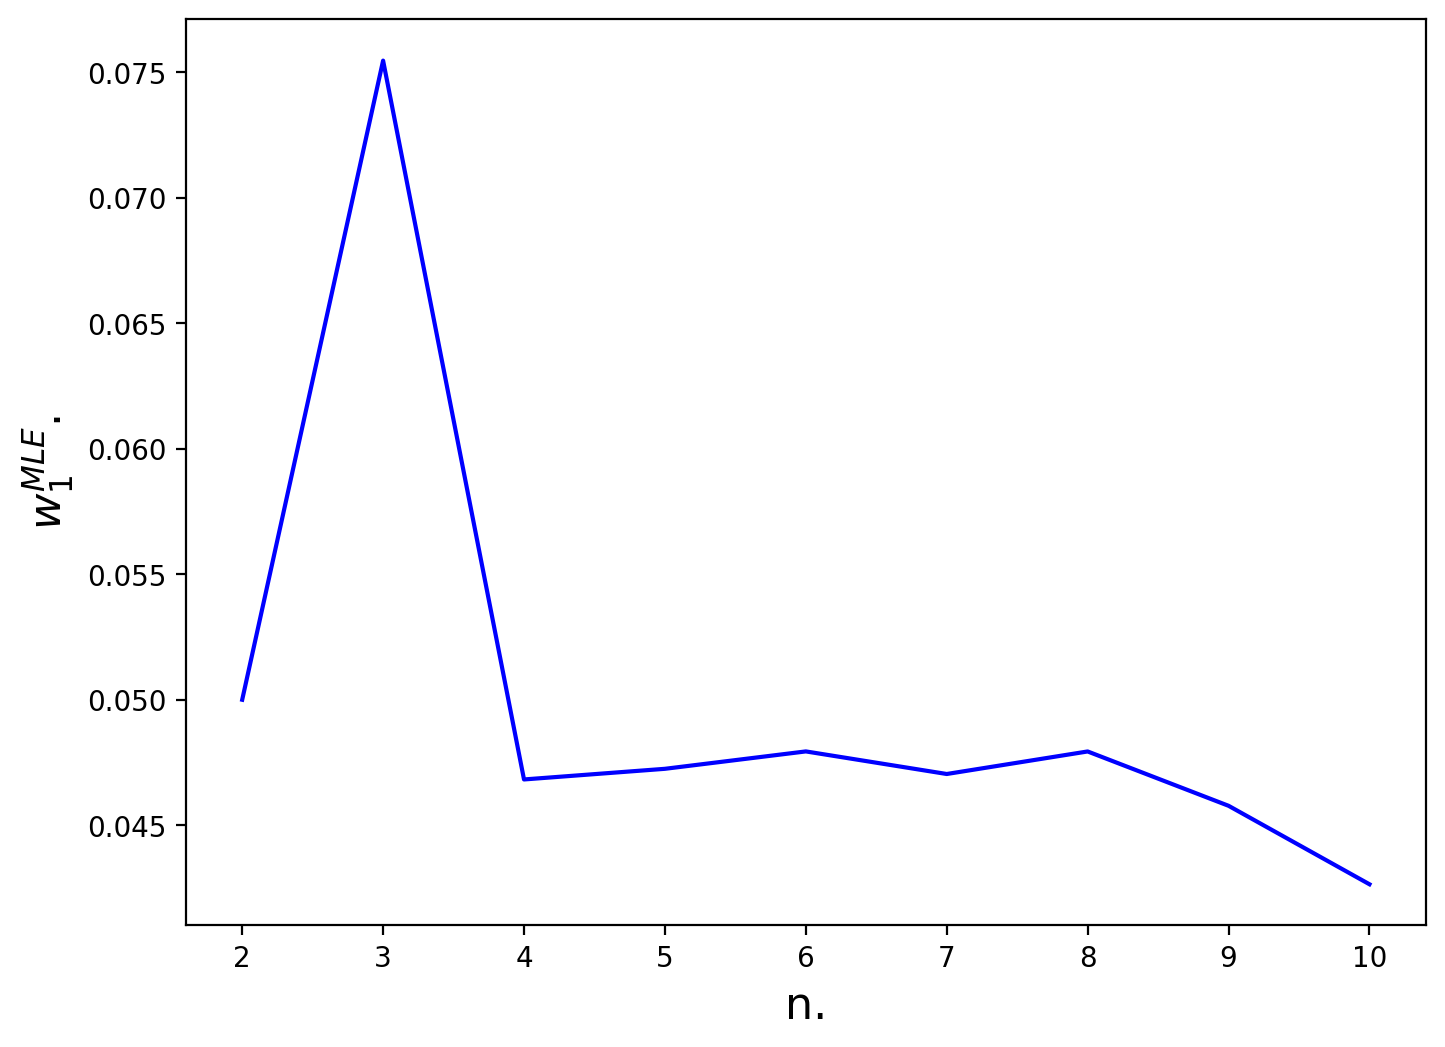
\includegraphics[width=7cm,height=5cm]{./figures/7-7-2.png}
\caption{Exercise 7.7. P2}
\end{figure}
Where we borrow data from exercise 7.8 for illustration.
The data in $x$ and $y$ appear in a sequential order for Figure. 7. 14.
That is to say, if we shuffle $x$ and $y$ accordingly, the estiamtion for weights is expected to converge faster.

\subsection{Bayesian linear regression in 1d with known $\sigma^{2}$}
For question (a), the estimation for $\sigma^{2}$ is $0.3173$.

For question (b), we have:
$$p(\textbf{w}) \propto \mathcal{N}(w_{1}|0,1) \propto \exp\left\{ -\frac{1}{2}w_{1}^{2} \right\}.$$
To simplify the algebra, we observe that $w_{1}$ and $w_{0}$ are independent in this prior.
Thus the prior distribution can be reduced to:
$\mathcal{N}(w_{1}|0,1)\cdot \mathcal{N}(w_{0}|\gamma,\infty),$
where $\gamma$ can be an arbitrary finite number, thus:
$$\textbf{m}_{0}=\begin{pmatrix}
0 \\
\gamma
\end{pmatrix},$$
$$\textbf{V}_{0}=\begin{pmatrix}
1 & 0 \\
0 & 0
\end{pmatrix}.$$

For question (c) and (d), we consider the posterior distribution for parameters:
$$
\begin{aligned}
p(\textbf{w}|\mathcal{D},\sigma^{2}) &=\mathcal{N}(\textbf{w}|\textbf{m}_{0},\textbf{V}_{0})\cdot\prod_{n=1}^{N}\mathcal{N}(y_{n}|w_{0}+w_{1}x_{n},\sigma^{2})\\
&\propto\exp\left\{-\frac{w^{2}_{1}}{2} \right\}\cdot \prod_{n=1}^{N}\exp\left\{-\frac{(y_{n}-w_{0}-w_{1}x_{n})^{2}}{2\sigma^{2}} \right\},
\end{aligned}
$$
where we only maintain terms dependent on $w_{0}$ and $w_{1}$.
To marginalize out $w_{0}$, we have:
$$
\begin{aligned}
p(w_{1}|\mathcal{D},\sigma^{2})&=\int p(w_{1},w_{0})\text{d}w_{0}\\
&\propto\exp\left\{-\frac{w_{1}^{2}}{2}\right\}\cdot\int \exp\left\{Aw_{1}^{2}+Bw_{0}^{2}+Cw_{0}w_{1}+Dw_{1}+Ew_{0}+F \right\}\text{d}w_{0}\\
&=\exp\left\{-\frac{w_{1}^{2}}{2}+Aw_{1}^{2}+Dw_{1}+F\right\}\cdot \int \exp\left\{Bw_{0}^{2}+Cw_{0}w_{1}+Ew_{0} \right\}\text{d}w_{0}\\
&=\exp\left\{-\frac{w_{1}^{2}}{2}+Aw_{1}^{2}+Dw_{1}+F-\frac{(Cw_{1}+E)^{2}}{4B}\right\}\cdot \\
&\int \exp\left\{Bw_{0}^{2}+(Cw_{1}+E)w_{0}+ \frac{(Cw_{1}+E)^{2}}{4B}\right\}\text{d}w_{0}\\
&\propto \exp\left\{-\frac{w_{1}^{2}}{2}+Aw_{1}^{2}+Dw_{1}+F-\frac{(Cw_{1}+E)^{2}}{4B}\right\}.
\end{aligned}
$$
Hence the posterior distribution over $w_{1}$ is a normal distribution.
The coefficients for $w_{1}^{2}$ and $w_{1}$ in the exponential are respectively:
$$-\frac{1}{2}+A-\frac{C^{2}}{4B},$$
$$D-\frac{CE}{2B}.$$
Thence its posterior variance is:
$$\frac{1}{1-2A+\frac{C^{2}}{2B}},$$
its mean is:
$$\frac{2BD-CE}{2B-4AB+C^{2}}.$$
Finally, let us plug $A$ to $E$ with statistics of $\mathcal{D}$:
$$
\begin{aligned}
A&=-\frac{\sum_{n=1}^{N}x_{n}^{2}}{2\sigma^{2}},\\
B&=-\frac{N}{2\sigma^{2}},\\
C&=-\frac{\sum_{n=1}^{N}x_{n}}{\sigma^{2}},\\
D&=\frac{\sum_{n=1}^{N}x_{n}y_{n}}{\sigma^{2}},\\
E&=\frac{\sum_{n=1}^{N}y_{n}}{\sigma^{2}}.
\end{aligned}
$$
The posterior variance is:
$$\frac{\sigma^{2}}{\sigma^{2}+\sum x^{2}-\frac{(\sum x)^{2}}{N}},$$
from which we observe that, with $N$ grows, the denominator increases as the bound from the Cauchy inequality:
$$\sum_{n=1}^{N}x_{n}^{2}-\frac{(\sum_{n=1}^{N}x_{n})^{2}}{N}\geq 0.$$
To put in other words, The larger the Cauchy difference is, the more confidence we have for the estimation of $w_{1}$.
Such difference is determined by the variance of the distribution on $x$.
The posterior variance can be reduced to:
$$\frac{\sigma^{2}}{\sigma^{2}+N\text{var}(x)}.$$
Therefore for any fixed generative distribution on $x$, the uncertainty on $w_{1}$ declines as $\mathcal{O}\left\{\frac{1}{N} \right\}$.


\subsection{Generative model for linear regression}
For question (a), assume that $\textbf{x}$ and $y$ are jointly subject to a Gaussian:
$$\mathcal{N}\left(\begin{pmatrix}\textbf{x}\\ y \end{pmatrix}|
\begin{pmatrix}\mu_{\textbf{x}}\\ \mu_{y} \end{pmatrix},
  \begin{pmatrix}\Sigma_{xx} & \Sigma_{xy} \\
                 \Sigma_{xy}^{\text{T}} & \Sigma_{yy} \end{pmatrix}
 \right).$$
We know from (4.68) that the marginal distribution of $\textbf{x}$ and $y$ are $\mathcal{N}(\textbf{x}|\mu_{\textbf{x}},\Sigma_{xx})$ and $\mathcal{N}(\textbf{y}|\mu_{y},\Sigma_{yy})$ respectively, this is sufficient for MLE $\mu_{\textbf{x}}$, $\mu_{y}$, $\Sigma_{xx}$ and $\Sigma_{yy}$:
$$
\begin{aligned}
\mu_{\textbf{x}}&=\frac{1}{N}\cdot\sum_{n=1}^{N}\textbf{x}_{n},\\
\mu_{y}&=\frac{1}{N}\cdot\sum_{n=1}^{N}y_{n},\\
\Sigma_{xx}&=\frac{1}{N}\cdot\sum_{n=1}^{N}(\textbf{x}_{n}-\bar{\textbf{x}})(\textbf{x}_{n}-\bar{\textbf{x}})^{\text{T}}=\frac{1}{N}\cdot\bar{\textbf{X}}\bar{\textbf{X}}^{\text{T}},\\
\Sigma_{yy}&=\frac{1}{N}\cdot\sum_{n=1}^{N}(y_{n}-\bar{y})^{2}=\frac{1}{N}\bar{\textbf{Y}}^{\text{T}}\bar{\textbf{Y}}.
\end{aligned}
$$
For an estimation of $\Sigma_{xy}$, connecting $\textbf{x}$ and $y$ together then estimating this vector's covariance matrix (this is an ordinary Gaussian model), picking only the first $D$ components from its last column:
$$\Sigma_{xy}=\frac{1}{N}\bar{\textbf{X}}\bar{\textbf{Y}}.$$

Finally, plugging our observations into (4.69):
$$\mu_{y|\textbf{x}}=\mu_{y}+\Sigma_{yx}\Sigma^{-1}_{xx}(\textbf{x}-\mu_{\textbf{x}}),$$
which equals:
$$\bar{y}+\frac{1}{N}\cdot\bar{\textbf{Y}}^{\text{T}}\bar{\textbf{X}}^{\text{T}}\cdot N\cdot (\bar{\textbf{X}}\bar{\textbf{X}}^{\text{T}})^{-1}\cdot(\textbf{x}-\bar{\textbf{x}}).$$
This is identical to what (7.109)-(7.111) implies, hence the proof is completed.

For question (b), there is no significant difference except that we are now equipped with a distribution of $x$.
This enables us the ability of generating more samples and sheds light on active querying strategies, in which we can query an oracle for samples in order to accelerate the convergence of the learning process.

\subsection{Bayesian linear regression using the g-prior}
For Bayesian linear regression model, the likelihood is as always:
$$p(\mathcal{D}|\textbf{w},\sigma^{2})=\prod_{n=1}^{N}\mathcal{N}(y_{n}|\textbf{w}^{\text{T}}\textbf{x}_{n},\sigma^{2}).$$
The prior distribution is Gaussian-Inverse Gamma distribution:
$$
\begin{aligned}
p(\textbf{w},\sigma^{2})&=\text{NIG}(\textbf{w},\sigma^{2}|\textbf{w}_{0},\textbf{V}_{0},a_{0},b_{0})\\
&=\mathcal{N}(\textbf{w}|\textbf{w}_{0},\sigma^{2}\textbf{V}_{0})\cdot\text{IG}(\sigma^{2}|a_{0},b_{0}) \\
&=\frac{1}{(2\pi)^{\frac{D}{2}}}\frac{1}{|\sigma^{2}\textbf{V}_{0}|^{\frac{1}{2}}}\exp\left\{ -\frac{1}{2}(\textbf{w}-\textbf{w}_{0})^{T}(\sigma^{2}\textbf{V}_{0})^{-1}(\textbf{w}-\textbf{w}_{0}) \right\} \cdot \\
&\ \ \ \frac{b_{0}^{a_{0}}}{\Gamma(a_{0})}(\sigma^{2})^{-(a_{0}+1)}\exp\left\{ -\frac{b_{0}}{\sigma^{2}} \right\} \\
&=\frac{b_{0}^{a_{0}}}{(2\pi)^{\frac{D}{2}}|\textbf{V}_{0}|^{\frac{1}{2}}\Gamma(a_{0})}(\sigma^{2})^{-\left(a_{0}+\frac{D}{2}+1\right)}\cdot\exp\left\{ -\frac{(\textbf{w}-\textbf{w}_{0})^{\text{T}}\textbf{V}_{0}^{-1}(\textbf{w}-\textbf{w}_{0})+2b_{0}}{2\sigma^{2}} \right\}.
\end{aligned}
$$
The posterior distribution takes the form:
$$
\begin{aligned}
p(\textbf{w},\sigma^{2}|\mathcal{D}) &\propto p(\textbf{w},\sigma^{2})p(\mathcal{D}|\textbf{w},\sigma^{2})\\
&\propto \frac{b_{0}^{a_{0}}}{(2\pi)^{\frac{D}{2}}|\textbf{V}_{0}|^{\frac{1}{2}}\Gamma(a_{0})}(\sigma^{2})^{-\left(a_{0}+\frac{D}{2}+1\right)}\cdot \\
&\ \ \ \exp\left\{ -\frac{(\textbf{w}-\textbf{w}_{0})^{\text{T}}\textbf{V}_{0}^{-1}(\textbf{w}-\textbf{w}_{0})+2b_{0}}{2\sigma^{2}} \right\} \cdot \\
&\ \ \ (\sigma^{2})^{-\frac{N}{2}}\cdot \exp\left\{ -\frac{\sum_{n=1}^{N}(y_{n}-\textbf{w}^{\text{T}}\textbf{x}_{n})^{2}}{2\sigma^{2}}  \right\}.
\end{aligned}
$$
To decompose the updated hyperparameters from this form, we have to find:
\begin{itemize}
\item The exponential of $\sigma^{2}$.
\item The squared term within the exponential.
\end{itemize}
The exponential of $\sigma^{2}$ in the posterior is:
$$-\left(a_{0}+\frac{D}{2}+1\right)-\frac{N}{2},$$
thus we have:
$$a_{N}=a_{0}+\frac{N}{2}=\frac{N}{2}.$$

The coefficient of $\textbf{w}^{\text{T}}\textbf{w}$ in the exponential (as the introducer matrix of the inner product) is:
$$-\frac{\textbf{V}_{0}^{-1}}{2\sigma^{2}}-\frac{\textbf{X}\textbf{X}^{\text{T}}}{2\sigma^{2}},$$
therfore:
$$\textbf{V}_{N}^{-1}=\textbf{V}_{0}^{-1}+\textbf{X}\textbf{X}^{\text{T}},$$
with $\textbf{V}_{0}=g(\textbf{X}\textbf{X}^{\text{T}})^{-1}$:
$$\textbf{V}_{N}=\frac{g}{g+1}\left(\textbf{X}\textbf{X}^{\text{T}} \right)^{-1}.$$

The coefficient of $\textbf{w}^{\text{T}}$ in the exponential is:
$$\frac{\textbf{V}_{0}^{-1}\textbf{w}_{0}}{\sigma^{2}}+\frac{\sum_{n=1}^{N}y_{n}\textbf{x}_{n}}{\sigma^{2}}=\frac{\textbf{V}_{0}^{-1}\textbf{w}_{0}}{\sigma^{2}}+\frac{\textbf{X}\textbf{Y}}{\sigma^{2}}.$$
So we have:
$$\textbf{V}_{0}^{-1}\textbf{w}_{0}+\textbf{X}\textbf{Y}=\textbf{V}_{N}^{-1}\textbf{w}_{N}.$$
This yields:
$$
\begin{aligned}
\textbf{w}_{N}&=\textbf{V}_{N}\left(\textbf{V}_{0}^{-1}\textbf{w}_{0}+\textbf{X}\textbf{Y} \right)\\
&=\frac{g}{g+1}\left(\textbf{X}\textbf{X}^{\text{T}} \right)^{-1}\left(\frac{\textbf{X}\textbf{X}^{\text{T}}}{g}\textbf{0}+\textbf{X}\textbf{Y} \right)\\
&=\frac{g}{g+1}\left(\textbf{X}\textbf{X}^{\text{T}} \right)^{-1}\textbf{X}\textbf{Y}.
\end{aligned}
$$

Finally, completing the square within the exponential yields:
$$(\textbf{w}-\textbf{w}_{0})^{\text{T}}\textbf{V}_{0}^{-1}(\textbf{w}-\textbf{w}_{0})+2b_{0}+(\textbf{w}^{\text{T}}\textbf{X}-\textbf{Y})^{2}=(\textbf{w}-\textbf{w}_{N})^{\text{T}}\textbf{V}_{N}^{-1}(\textbf{w}-\textbf{w}_{N})+2b_{N}.$$
Plugging in what we have already known about $\textbf{w}_{N}$ and $\textbf{V}_{N}$ results in:
$$b_{N}=\frac{\textbf{Y}^{\text{T}}\textbf{Y}}{2}+\frac{g}{2(g+1)}\textbf{w}_{\text{MLE}}^{\text{T}}\textbf{X}\textbf{X}^{\text{T}}\textbf{w}_{\text{MLE}}.$$
Now we have (7.113)-(7.116) established.


\newpage
\section{Logistic regression}
The logistic regression is the basic form of classification, which is the fundemantal task of machine intelligence.
Even for classifying complex data structures, the last layers of the model are usually logistic structures.

\subsection{Spam classification using logistic regression}
Practice by yourself.
I know nothing about \texttt{MATLAB}.

\subsection{Spam classification using naive Bayes}
Practice by yourself.

\subsection{Gradient and Hessian of log-likelihood for logistic regression}
For question (a),
$$\frac{\text{d}}{\text{d} a} \sigma(a) = \frac{\exp(-a)}{(1+\exp(-a))^{2}} = \frac{1}{1+\text{e}^{-a}}\frac{\text{e}^{-a}}{1+\text{e}^{-a}}=\sigma(a)\cdot (1-\sigma(a)).$$

For question (b),
\begin{align}
g(\textbf{w})=&\frac{\partial}{\partial \textbf{w}}\text{NLL}(\textbf{w})\nonumber \\
=&-\sum_{n=1}^{N}\frac{\partial}{\partial \textbf{w}} [y_{i}\log \mu_{i} + (1-y_{i})\log (1-\mu_{i})]\nonumber \\
=&-\sum_{n=1}^{N}y_{i}\frac{1}{\sigma_{i}}\sigma_{i}(1-\sigma_{i})\cdot\textbf{x}_{i}+(1-y_{i})\frac{-1}{1-\sigma_{i}}\sigma(1-\sigma_{i})\cdot\textbf{x}_{i}\nonumber \\
=&\sum_{n=1}^{N}(\sigma(\textbf{w}^{\text{T}}\textbf{x}_{i})-y_{i})\textbf{x}_{i},\nonumber
\end{align}
where $\sigma_{i}=\sigma(\textbf{w}^{\text{T}}\textbf{x}_{i})$.

For question (c), the results is obvious.
For an arbitrary vector $\textbf{u}$:
$$
\begin{aligned}
\textbf{u}^{\text{T}}\textbf{H}\textbf{u}&=\left(\textbf{X}\textbf{u}\right)^{\text{T}}\textbf{S}\left(\textbf{X}\textbf{u}\right)\\
&=\textbf{v}^{\text{T}}\textbf{S}\textbf{v}\\
&=\sum_{d=1}^{D}v_{d}^{2}\cdot\mu_{d}\cdot (1-\mu_{i})\geq 0.
\end{aligned}
$$
Hence $\textbf{H}$ is positive definite if all $\mu_{i}$ are within $(0,1)$, otherwise it is semi-positive definite.

\subsection{Gradient and Hessian of log-likelihood for multinomial logistic regression}
For question (a), given a sample indexed $i$,
$$\mu_{ik}=\frac{\exp(\textbf{w}_{k}^{\text{T}}\textbf{x}_{i})}{\sum_{c}\exp(\textbf{w}_{c}^{\text{T}}\textbf{x}_{i})},$$
$$\eta_{ij}=\textbf{w}_{j}^{\text{T}}\textbf{x}_{i}.$$
Now we have:
$$
\begin{aligned}
\frac{\partial \mu_{ik}}{\partial \eta_{ij}}&=\frac{\frac{\partial \exp(\eta_{ik})}{\partial \eta_{ij}}\cdot \sum_{c}\exp(\eta_{ic}) - \frac{\partial \sum_{c}\exp(\eta_{ic})}{\partial \eta_{ij}}\cdot\exp(\eta_{ik}) }{\left(\sum_{c}\exp(\eta_{ic}) \right)^{2}} \\
&=\frac{\exp\left(\eta_{ik}\right)\cdot\delta_{kj}\cdot \sum_{c}\exp(\eta_{ic})  - \exp\left(\eta_{ij}\right)\cdot \exp(\eta_{ik})}{\left(\sum_{c}\exp(\eta_{ic}) \right)^{2}}\\
&=\mu_{ik}\cdot\delta_{kj}-\mu_{ij}\cdot\mu_{ik},
\end{aligned}
$$
what dominates is but the elementary calculus.

For question (b), recall that:
$$l(\textbf{W})=\sum_{i=1}^{N}\sum_{c}y_{ic}\cdot \log \mu_{ic}.$$
Let $l_{i}(\textbf{W})=\sum_{c}y_{ic}\cdot\log \mu_{ic}$, we are now ready for reduction:
$$
\begin{aligned}
\frac{\partial l_{i}}{\partial \textbf{w}_{j}}&=\frac{\partial }{\partial \textbf{w}_{j}} \sum_{c}y_{ic}\cdot\log \mu_{ic} \\
&=\sum_{c}\frac{y_{ic}}{\mu_{ic}}\cdot\frac{\partial\mu_{ic}}{\partial\eta_{ij}}\cdot\frac{\partial\eta_{ij}}{\partial\textbf{w}_{j}}\\
&=\sum_{c}\frac{y_{ic}}{\mu_{ic}}\cdot\mu_{ic}\cdot(\delta_{cj}-\mu_{ij})\cdot\textbf{x}_{i}\\
&=\sum_{c}y_{ic}\cdot(1-\mu_{ij})\cdot\textbf{x}_{i}\\
&=y_{ij}\cdot(1-\mu_{ij})\cdot\textbf{x}_{i}-\sum_{c\neq j}y_{ic}\cdot\mu_{ij}\cdot\textbf{x}_{i}\\
&=y_{ij}\cdot(1-\mu_{ij})\cdot\textbf{x}_{i}+(y_{ij}-1)\cdot\mu_{ij}\cdot\textbf{x}_{i}\\
&=(y_{ij}-\mu_{ij})\cdot\textbf{x}_{i}.
\end{aligned}
$$
Summarizing over $i$ yields (8.126).

For question (c), we have by definition:
$$\textbf{H}_{c,c'}=\nabla_{\textbf{w}_{c'}}\nabla_{\textbf{w}_{c}}l(\textbf{W}).$$
Hence we begin with the result from question (b):
$$
\begin{aligned}
\nabla_{\textbf{w}_{c'}}\nabla_{\textbf{w}_{c}}l_{i}&=\frac{\partial}{\partial \textbf{w}_{c'}}(y_{ic}-\mu_{ic})\cdot\textbf{x}_{i}\\
&=-\frac{\partial }{\partial \textbf{w}_{c'}}\mu_{ic}\cdot\textbf{x}\\
&=-\frac{\partial\mu_{ic}}{\partial \eta_{ic'}}\frac{\partial \eta_{ic'}}{\partial \textbf{w}_{c'}}\cdot\textbf{x}_{i}\\
&=-\mu_{ic}(\delta_{cc'}-\mu_{ic'})\cdot\textbf{x}_{i}\textbf{x}_{i}^{\text{T}},
\end{aligned}
$$
where in the last step we have to adopt the outer product to span the Hessian.
Summarizing over $i$ yields the desired result (8.127).

\subsection{Symmetric version of l2 regularized multinomial logistic regression}
We borrow the results from exercise 8.5.
Once the $l_{2}$ prior is introduced, the likelihood becomes:
$$l_{2}=l-\sum_{c}\lambda\textbf{w}_{c}^{\text{T}}\textbf{w}_{c}.$$
Therefore (8.126) becomes:
$$\nabla_{\textbf{w}_{c}}l_{2}=\sum_{i}(y_{ic}-\mu_{ic})\cdot\textbf{x}_{i}-\lambda\textbf{w}_{c}.$$
At the unique optimum we have $\forall c$,
$$\nabla_{\textbf{w}_{c}}l_{2}=0,$$
which is identical to:
$$\hat{w}_{c,j}=\frac{1}{\lambda}\sum_{i}(y_{ic}-\mu_{ic})\cdot x_{ij}.$$
Therefore:
$$\sum_{c}\hat{w}_{c,j}=\frac{1}{\lambda}\sum_{i}\left[\sum_{c}(y_{ic}-\mu_{ic})\right]x_{ij},$$
whose value is zero since $\sum_{c}y_{ic}=\sum_{c}\mu_{ic}=1$.

\subsection{Elementary properties of l2 regularized logistic regression}
For question (a), the Hessian of $l_{2}$ regularized negative log likelihood is:
$$\textbf{H}+\lambda \textbf{I},$$
where $\textbf{H}$, following the derivation in exercise 8.3, is at least semi-positive definite.
So the Hessian for this model is strictly (for non-trivial $\lambda$) positive definite, there is a unique optimal solution.
The answer is False.

For question (b), the result is not necessarily true.
For a sparse optimum, one should resort to LASSO model, where a Laplace prior is exerted on weights.

For question (c), if $\lambda=0$ then the model reduces to ordinary logistic regression.
If the dataset is linearly separable then there exists $\textbf{w}'$ such that $\forall i$:
$$\textbf{w}'^{\text{T}}\textbf{x}_{i}\cdot y_{i}\geq 0.$$
Now for an arbitrary number $\alpha>0$, the weights $\alpha\cdot\textbf{w}'$ also meets the separation condition.
Let $\alpha\rightarrow\infty$ justifies that the statement in (c) is True.

For question (d), the statement is obvious False since the model now has to trade-off between fitness and prior knowledge.
Concretely, we can prove the other statement: \emph{as we increase $\lambda$, the likelihood on the train dataset monotonically decreases}.

Assume that $\hat{\textbf{w}}_{1}$ minimize the (8.131) with $\lambda_{1}$, denoted by $J_{1}$.
Now increase $\lambda_{1}$ to $\lambda_{2}$, we are now optimizing the loss:
$$J_{2}(\textbf{w})=-l(\textbf{w},\mathcal{D}_{\text{train}})+\lambda_{2}\textbf{w}^{\text{T}}\textbf{w},$$
whose optimal solution is denoted by $\hat{\textbf{w}}_{2}$.

If $\hat{\textbf{w}}_{1}=\hat{\textbf{w}}_{2}$ then we already have:
$$l(\hat{\textbf{w}}_{1},\mathcal{D}_{\text{train}})=l(\hat{\textbf{w}}_{2},\mathcal{D}_{\text{train}}).$$
Otherwise, we would have:
$$-l(\hat{\textbf{w}}_{1},\mathcal{D}_{\text{train}})+\lambda_{2}\hat{\textbf{w}}_{1}^{\text{T}}\hat{\textbf{w}_{1}} > -l(\hat{\textbf{w}}_{2},\mathcal{D}_{\text{train}})+\lambda_{2}\hat{\textbf{w}}_{2}^{\text{T}}\hat{\textbf{w}_{2}}.$$
If $l(\hat{\textbf{w}}_{2},\mathcal{D}_{\text{train}}) > l(\hat{\textbf{w}}_{1},\mathcal{D}_{\text{train}})$ then we would have:
$$\Delta=l(\hat{\textbf{w}}_{2},\mathcal{D}_{\text{train}})-l(\hat{\textbf{w}}_{1},\mathcal{D}_{\text{train}})>\lambda_{2}(\hat{\textbf{w}}_{2}^{\text{T}}\hat{\textbf{w}_{2}}-\hat{\textbf{w}}_{1}^{\text{T}}\hat{\textbf{w}_{1}}).$$
Finally, consider:
$$J_{1}(\hat{\textbf{w}}_{1})-J_{1}(\hat{\textbf{w}}_{2})=\Delta+\lambda_{1}(\hat{\textbf{w}}_{1}^{\text{T}}\hat{\textbf{w}_{1}}-\hat{\textbf{w}}_{2}^{\text{T}}\hat{\textbf{w}_{2}}).$$
If $\hat{\textbf{w}}_{1}^{\text{T}}\hat{\textbf{w}_{1}}>\hat{\textbf{w}}_{2}^{\text{T}}\hat{\textbf{w}_{2}}$ then $\hat{\textbf{w}}_{1}$ is not the optimum of $J_{1}$ and we arrive in a contradiction.
Otherwise:
$$\lambda_{1}(\hat{\textbf{w}}_{2}^{\text{T}}\hat{\textbf{w}_{2}}-\hat{\textbf{w}}_{1}^{\text{T}}\hat{\textbf{w}_{1}})<\lambda_{2}(\hat{\textbf{w}}_{2}^{\text{T}}\hat{\textbf{w}_{2}}-\hat{\textbf{w}}_{1}^{\text{T}}\hat{\textbf{w}_{1}})<\Delta.$$
Hence we still have the optimality of $\hat{\textbf{w}}_{1}$ fail.
This finishes the proof.

For question (e), the statement is False.
This can be easily shown by imagine $\lambda\rightarrow\infty$.

\subsection{Regularizing separate terms in 2d logistic regression}
The decision boundary is given by:
$$w_{0}+w_{1}\cdot x_{1}+w_{2}\cdot x_{2}=0,$$
hence a straight line in the $X_{1}-X_{2}$ plane.

For question (a), the decision boundary is an arbitrary line.

For question (b), the decision boundary is a line that passes the origin.

For question (c), the decision boundary is a line parallel to the $X_{1}$ axis.

For question (c), the decision boundary is a line parallel to the $X_{2}$ axis.

\newpage
\section{Generalized linear models and the exponential family}
\subsection{Conjugate prior for univariate Gaussian in exponential family form}
The 1d Gaussian distribution is:
$$N(x|\mu,\sigma^{2})=\frac{1}{\sqrt{2\pi \sigma^{2}}}\exp\left\{-\frac{1}{2\sigma^{2}}(x-\mu)^{2} \right\}$$

Rewrite it into:
$$p(x|\mu,\sigma^{2})=\exp\left\{-\frac{1}{2\sigma^{2}}x^{2} + \frac{1}{\sigma^{2}}x -\left\{\frac{\mu^{2}}{2\sigma^{2}}+\frac{\ln(2\pi\sigma^{2})}{2}\right\}  \right\}$$

Denote $\theta = (-\frac{\lambda}{2},\lambda\mu)^{T}$,$A(\theta) =\frac{\lambda\mu^{2}}{2}+\frac{\ln(2\pi)}{2}-\frac{\ln \lambda}{2}$,$\phi(x)=(x^{2},x)^{T}$. Consider the likelihood with dataset$D$:
$$\log p(D|\theta) = \exp\left\{ \theta^{T}(\sum_{n=1}^{N}\phi(x_{n})) -N\cdot A(\theta) \right\}$$

According to the meaning of prior distribution, we set a observation background in order to define a prior distribution. The sufficient statistics is the only thing matters by the form of exponential family. Assume that we have $M$ prior observations. The mean of them and their square are 为$v_{1}$ and $v_{2}$ respectively, then the prior distribution takes the form:
$$p(\theta|M,v_{1},v_{2})=\exp\left\{ \theta_{1}\cdot Mv_{1} + \theta_{2}\cdot Mv_{2} - M\cdot A(\theta) \right\}$$
$$=\exp\left\{-\frac{\lambda}{2}Mv_{1}+\lambda\mu Mv_{2} - \frac{M}{2}\lambda\mu^{2}-\frac{M}{2}\ln 2\pi + \frac{M}{2}\ln \lambda  \right\}$$

It has three independent parameters. We are to prove that is equals $p(\mu,\lambda)=N(\mu|\gamma,\frac{1}{\lambda(2\alpha-1)})Ga(\lambda|\alpha,\beta)$. Expand it into exponential form and ignore the terms independent with $\mu,\lambda$:
$$p(\mu,\lambda)=\exp\left\{ (\alpha-1)\ln \lambda - \beta\lambda -\frac{\lambda(2\alpha-1)}{2}\mu^{2}-\frac{\lambda(2\alpha-1)}{2}\gamma^{2}\right\}$$
$$\cdot\exp\left\{\lambda(2\alpha-1)\mu\gamma+\frac{1}{2}\ln \lambda \right\}$$

Compare the coefficients for $\lambda \mu^{2},\lambda \mu,\lambda,\ln \lambda$, we obtain:
$$-\frac{(2\alpha-1)}{2} = -\frac{M}{2}$$
$$\gamma(2\alpha-1)=Mv_{2}$$
$$\frac{(2\alpha-1)}{2}\gamma^{2}-\beta=-\frac{1}{2}Mv_{1}$$
$$(\alpha-1)+\frac{1}{2}=\frac{M}{2}$$

Combining them ends in:
$$\alpha = \frac{M+1}{2}$$
$$\beta = \frac{M}{2}(v_{2}^{2}+v_{1})$$
$$\gamma = v_{2}$$

Thus two distributions are equal with naive change of variables' names.

\subsection{The MVN is in the exponential family}
Here you can find a comprehensive solution:

\url{https://stats.stackexchange.com/questions/231714/sufficient-statistic-for-multivariate-normal}.

\newpage
\section{Directed graphical models(Bayes nets)}
...

\newpage
\section{Mixture models and the EM algorithm}
\subsection{Student T as infinite mixture of Gaussian}
The 1d Student-t distribution takes the form:
$$St(x|\mu,\sigma^{2},v)=\frac{\Gamma(\frac{v}{2}+\frac{1}{2})}{\Gamma(\frac{v}{2})}(\frac{1}{\pi v \sigma^{2}})^{\frac{1}{2}}(1+\frac{(x-\mu)^{2}}{v\sigma^{2}})^{-\frac{v+1}{2}}$$

Consider the left side of 11.61:
\begin{align}
 & \int N(x|\mu,\frac{\sigma^{2}}{z})Ga(z|\frac{v}{2},\frac{v}{2})dz \nonumber \\
=&\int \frac{\sqrt{z}}{\sqrt{2\pi\sigma^{2}}}\exp\left\{ -\frac{z}{2\sigma^{2}}(x-\mu)^{2} \right\}\frac{(\frac{v}{2})^{\frac{v}{2}}}{\Gamma(\frac{v}{2})}z^{\frac{v}{2}-1}\exp\left\{ -\frac{v}{2}z \right\}dz \nonumber \\
=&\frac{1}{\sqrt{2\pi \sigma^{2}}}\frac{(\frac{v}{2})^{\frac{v}{2}}}{\Gamma(\frac{v}{2})}\int z^{\frac{v-1}{2}}\exp\left\{ -(\frac{v}{2}+\frac{(x-\mu)^{2}}{2\sigma^{2}})z \right\} dz \nonumber
\end{align}

The integrated function is the terms related to $z$ in Gamma distribution $Ga(z|\frac{v+1}{2},\frac{(x-\mu)^{2}}{2\sigma^{2}}+\frac{v}{2})$, which gives to the normalized term's inverse.
$$\int z^{\frac{v-1}{2}}\exp\left\{ -(\frac{v}{2}+\frac{(x-\mu)^{2}}{\sigma^{2}})z \right\} dz = \Gamma(\frac{v+1}{2})(\frac{(x-\mu)^{2}}{2\sigma^{2}}+\frac{v}{2})^{-\frac{v+1}{2}}$$

Plug in can derive 11.61.

\subsection{EM for mixture of Gaussians}
We are to optimize:
\begin{align}
Q(\theta,\theta^{old})=&\mathbb{E}p(z|D,\theta^{old})[\sum_{n=1}^{N}\log (\textbf{x}_{n},\textbf{z}_{n}|\theta)]\nonumber \\
=&\sum_{n=1}^{N}\mathbb{E}[\log \prod_{k=1}^{K}(\pi_{k}p(\textbf{x}_{n}|z_{k},\theta))^{z_{nk}}]\nonumber \\
=&\sum_{n=1}^{N}\sum_{k=1}^{K}r_{nk}\log (\pi_{k}p(\textbf{x}_{n}|z_{k},\theta))\nonumber
\end{align}

Where:
$$r_{nk}=p(z_{nk}=1|\textbf{x}_{n},\theta^{old})$$

When the emission distribution $p(\textbf{x}|z,\theta)$ is Gaussian, consider the terms involve$\mu_{k}$ in $Q(\theta,\theta^{old})$ first:
$$\sum_{n=1}^{N}r_{nk} \log p(\textbf{x}_{n}|z_{k},\theta) = \sum_{n=1}^{N} r_{nk} (-\frac{1}{2})(\textbf{x}_{n}-\mu_{k})^{T}\Sigma^{-1}(\textbf{x}_{n}-\mu_{k}) + C$$

Setting the derivative to zero results in:
$$\sum_{n=1}^{N}r_{nk}(\mu_{k}-\textbf{x}_{n})=0$$

And we obtain 11.31:
$$\mu_{k} =\frac{\sum_{n=1}^{N}r_{nk}\textbf{x}_{n}}{\sum_{n=1}^{N}r_{nk}}$$

For terms involve $\Sigma_{k}$ in $Q(\theta,\theta^{old})$:
$$\sum_{n=1}^{N}r_{nk}\log p(\textbf{x}_{n}|z_{k},\theta) = \sum_{n=1}^{N}r_{nk} (-\frac{1}{2})(\log |\Sigma_{k}|+(\textbf{x}_{n}-\mu_{k})^{T}\Sigma^{-1}(\textbf{x}_{n}-\mu_{k})) + C$$

Using the same way as in 4.1.3.1:
$$L(\Sigma^{-1}=\Lambda)=(\sum_{n=1}^{N}r_{nk})\log |\Lambda|-Tr\left\{ (\sum_{n=1}^{N}r_{nk}(\textbf{x}_{n}-\mu_{k})(\textbf{x}_{n}-\mu_{k})^{T}) \Lambda \right\}$$

The balance condition is:
$$(\sum_{n=1}^{N}r_{nk})\Lambda^{-T}=\sum_{n=1}^{N}r_{nk}(\textbf{x}_{n}-\mu_{k})(\textbf{x}_{n}-\mu_{k})^{T}$$

Obtain 11.32:
$$\Sigma_{k} = \frac{\sum_{n=1}^{N}r_{nk}(\textbf{x}_{n}-\mu_{k})(\textbf{x}_{n}-\mu_{k})^{T}}{\sum_{n=1}^{N}r_{nk}}$$

\subsection{EM for mixtures of Bernoullis}
During the MLE for mixtures of Bernoullis, consider($D=2$ marks the number of  potential elements):
\begin{align}
\frac{\partial}{\partial \mu_{kj}}\sum_{n=1}^{N}\sum_{k=1}^{K}r_{nk}\log p(\textbf{x}_{n}|\theta,k)=&\sum_{n=1}^{N}r_{nk}\frac{\partial}{\partial \mu_{kj}}(\sum_{i}^{D}x_{ni}\log \mu_{ki})\nonumber \\
=&\sum_{n=1}^{N}r_{nk}x_{nj}\frac{1}{\mu_{kj}}\nonumber
\end{align}

Introduce a multipler to constrain $\sum_{j}\mu_{kj}=1$, then condition for the derivative to be zero is:
$$\mu_{kj}=\frac{\sum_{n=1}^{N}r_{nk}x_{nj}}{\lambda}$$

Summer over all $j$:
$$1=\sum_{j=1}^{D}\mu_{kj} = \frac{1}{\lambda}\sum_{j=1}^{D}\sum_{n=1}^{N}r_{nk}x_{nj}=\frac{1}{\lambda}\sum_{n=1}^{N}r_{nk}\sum_{j=1}^{D}x_{nj}=\frac{\sum_{n=1}^{N}r_{nk}}{\lambda}$$

Results in:
$$\lambda = \sum_{n=1}^{N}r_{nk}$$

Hence 11.116。

Introduce a prior:
$$p(\mu_{k0})\propto \mu_{k0}^{\alpha-1}\mu_{k1}^{\beta-1}$$

The zero-derivative condition becomes:
$$\mu_{k0}=\frac{\sum_{n=1}^{N}r_{nk}x_{n0}+\alpha-1}{\lambda}$$
$$\mu_{k1}=\frac{\sum_{n=1}^{N}r_{nk}x_{n1}+\beta-1}{\lambda}$$

And:
$$1=\mu_{k0}+\mu_{k1}=\frac{1}{\lambda}(\sum_{n=1}^{N}r_{nk}(x_{n0}+x_{n1})+\alpha+\beta-2)$$
$$\lambda = \sum_{n=1}^{N}r_{nk}+\alpha+\beta-2$$

Hence 11.117。

\subsection{EM for mixture of Student distributions}
The log-likelihood for complete data set is:
$$l_{c}(\textbf{x},z)=\log(N(\textbf{x}|\mu,\frac{\Sigma}{z})Ga(z|\frac{\lambda}{2},\frac{\lambda}{2}))$$
$$=-\frac{D}{2}\log(2\pi)-\frac{1}{2}\log|\Sigma|+\frac{D}{2}\log(z)-\frac{z}{2}(\textbf{x}-\mu)^{T}\Sigma^{-1}(\textbf{x}-\mu)+$$
$$\frac{v}{2}\log (\frac{v}{2}) -\log(\Gamma(\frac{v}{2}))+(\frac{v}{2}-1)\log (z) - \frac{v}{2}z$$

Sum the terms involving $v$:
$$l_{v}(\textbf{x},z)=\frac{v}{2}\log(\frac{v}{2})-\log(\Gamma(\frac{v}{2}))+\frac{v}{2}(\log(z)-z)$$

The likelihood w.r.t $v$ on complete data set is:
$$L_{v}=\frac{vN}{2}\log(\frac{v}{2})-N\log(\Gamma(\frac{v}{2}))+\frac{v}{2}\sum_{n=1}^{N}(\log(z_{n})-z_{n})$$

Setting derivative to zero gives:
$$\frac{\nabla\Gamma(\frac{v}{2})}{\Gamma(\frac{v}{2})}-1-\log(\frac{v}{2})=\frac{\sum_{n=1}^{N}(\log(z_{n})-z_{n})}{N}$$

For $\mu$ and $\Sigma$:
$$l_{\mu,\Sigma}(\textbf{x},z)=-\frac{1}{2}\log|\Sigma|-\frac{z}{2}(\textbf{x}-\mu)^{T}\Sigma^{-1}(\textbf{x}-\mu)$$
$$L_{\mu,\Sigma}=\frac{N}{2}\log|\Sigma|-\frac{1}{2}\sum_{n=1}^{N}z_{n}(\textbf{x}_{n}-\mu)^{T}\Sigma^{-1}(\textbf{x}_{n}-\mu)$$

Hence equals the MLE used for MVN.

\subsection{Gradient descent for fitting GMM}
From the given information:
$$p(\textbf{x}|\theta)=\sum_{k}\pi_{k}N(\textbf{x}|\mu_{k},\Sigma_{k})$$
$$l(\theta)=\sum_{n=1}^{N}\log p(\textbf{x}_{n}|\theta)$$

Deriavte w.r.t $\mu_{k}$:
\begin{align}
\frac{\partial}{\partial \mu_{k}}l(\theta) =& \sum_{n=1}^{N}\frac{\pi_{k}N(\textbf{x}_{n}|\mu_{k},\Sigma_{k})\nabla_{\mu_{k}}\left\{-\frac{1}{2}(\textbf{x}_{n}-\mu_{k})^{T}\Sigma_{k}^{-1}(\textbf{x}_{n}-\mu_{k})  \right\}}{\sum_{k'=1}^{K}\pi_{k'}N(\textbf{x}_{n}|\mu_{k'},\Sigma_{k'})}\nonumber \\
=&\sum_{n=1}^{N}r_{nk}\Sigma_{k}^{-1}(\textbf{x}_{n}-\mu_{k})\nonumber
\end{align}

w.r.t $\pi_{k}$:
$$\frac{\partial}{\partial \pi_{k}}l(\theta)=\sum_{n=1}^{N}\frac{N(\textbf{x}_{n}|\mu_{k},\Sigma^{k})}{\sum_{k'=1}^{K}\pi_{k'}N(\textbf{x}_{n}|\mu_{k'},\Sigma_{k'})}=\frac{1}{\pi_{k}}\sum_{n=1}^{N}r_{nk}$$

Using Languarge multipler ends in:
$$\pi_{k}=\frac{\sum_{n=1}^{N}r_{nk}}{\lambda}$$

Sum over $k$ and normalize:
$$\pi_{k}=\frac{\sum_{n=1}^{N}r_{nk}}{N}$$

For $\Sigma_{k}$:
$$\frac{\partial}{\partial \Sigma_{k}}l(\theta)=\sum_{n=1}^{N}\frac{\pi_{k}\nabla_{\Sigma_{k}}N(\textbf{x}_{n}|\mu_{k},\Sigma_{k})}{\sum_{k'=1}^{K}pi_{k'}N(\textbf{x}_{n}|\mu_{k'},\Sigma_{k'})}$$

Where:
$$\nabla_{\Sigma_{k}}N(\textbf{x}|\mu_{k},\Sigma_{k})=\frac{1}{(2\pi)^{\frac{D}{2}}}\frac{1}{|\Sigma_{k}|^{\frac{1}{2}}}\exp\left\{ -\frac{1}{2}(\textbf{x}-\mu_{k})^{T}\Sigma_{k}^{-1}(\textbf{x}-\mu_{k}) \right\}\nabla_{\Sigma_{k}}\cdot$$
$$\left\{ \nabla_{\Sigma_{k}}(-\frac{1}{2}(\textbf{x}-\mu_{k})\Sigma_{k}^{-1}(\textbf{x}-\mu_{k}))-\Sigma_{k}^{-1}\nabla_{\Sigma_{k}}|\Sigma_{k}| \right\}$$
$$=N(\textbf{x}|\mu_{k},\Sigma_{k})\nabla(\log N(\textbf{x}|\mu_{k},\Sigma_{k}))$$

Thus we have:
$$\Sigma_{k}=\frac{\sum_{n=1}^{N}r_{nk}(\textbf{x}_{n}-\mu_{k})(\textbf{x}_{n}-\mu_{k})^{T}}{\sum_{n=1}^{N}r_{nk}}$$

\subsection{EM for a finite scale mixture of Gaussians}
$J$ and $K$ are independent, using Bayes' rules(we have omitted $\theta$ in condition w.l.o.g):
\begin{align}
p(J_{n}=j,K_{n}=k|x_{n})=&\frac{p(J_{n}=j,K_{n}=k,x_{n})}{p(x_{n})}\nonumber \\
=&\frac{p(J_{n}=j)p(K_{n}=k)p(x_{n}|J_{n}=j,K_{n}=k)}{\sum_{J_{n},K_{n}}p(J_{n},K_{n},x_{n})}\nonumber \\
=&\frac{p_{j}q_{k}N(x_{n}|\mu_{j},\sigma^{2}_{k})}{\sum_{J_{n}=1}^{m}\sum_{K_{n}=1}^{l}p_{J_{n}}q_{K_{n}}N(x_{n}|\mu_{J_{n}},\sigma^{2}_{K_{n}})}\nonumber
\end{align}

Derive the form of auxiliary fucntion $Q(\theta^{new},\theta^{old})$:
\begin{align}
Q(\theta^{new},\theta^{old})=&\mathbb{E}_{\theta^{old}}\sum_{n=1}^{N}\log p(x_{n},J_{n},K_{n}|\theta^{new})\nonumber \\
=&\sum_{n=1}^{N}\mathbb{E}[\log(\prod_{j=1}^{m}\prod_{k=1}^{l} p(x_{n},J_{n},K_{n}|\theta^{new})^{\mathbb{I}(J_{n}=j,K_{n}=k)} )]\nonumber \\
=&\sum_{n=1}^{N}\sum_{j=1}^{m}\sum_{k=1}^{l}\mathbb{E}(\mathbb{I}(J_{n}=j,K_{n}=k))(\log p_{j} + \log q_{k} + \log N(x_{n}|\mu_{j},\sigma^{2}_{k}))\nonumber \\
=&\sum_{n,j,k}r_{njk}\log p_{j} + \sum_{n,j,k}r_{njk}\log q_{k} + \sum_{njk}r_{njk}\log N(x_{n}|\mu_{j},\sigma^{2}_{k})\nonumber
\end{align}

We are to optimize parameters $p,q,\mu,\sigma^{2}$. It is noticealbe that $p$ and $q$ can be optimized independently. Now fix $\sigma^{2}$ and optimize $\mu$:
\begin{align}
\frac{\partial}{\partial \mu_{j}}\sum_{n,j',k}r_{nj'k}N(x_{n}|\mu_{j},\sigma^{2}_{k})=&\sum_{n,k}r_{njk}\nabla_{\mu_{k}}N(x_{n}|\mu_{j},\sigma^{2}_{k})\nonumber \\
=&\sum_{n,k}r_{njk}N(x_{n}|\mu_{j},\sigma^{2}_{k})\frac{x_{n}-\mu_{j}}{\sigma^{2}_{k}}\nonumber
\end{align}

And we ends in:
$$\mu_{j}=\frac{\sum_{n,k}r_{njk}N(x_{n}|\mu_{j},\sigma^{2}_{k})\frac{x_{n}}{\sigma^{2}_{k}}} { \sum_{n,k}r_{njk}N(x_{n}|\mu_{j},\sigma^{2}_{k})\frac{1}{\sigma^{2}_{k}}}$$

\subsection{Manual calculation of the M step for a GMM}
Practise by yourself.

\subsection{Moments of a mixture of Gaussians}
For the expectation of mixture distribution:
\begin{align}
\mathbb{E}(\textbf{x})=&\int\textbf{x}\sum_{k}\pi_{k}N(\textbf{x}|\mu_{k},\Sigma_{k})d\textbf{x}\nonumber \\
=&\sum_{k}\pi_{k}(\int\textbf{x}N(\textbf{x}|\mu_{k},\Sigma_{k})d\textbf{x})\nonumber \\
=&\sum_{k}\pi_{k}\mu_{k}\nonumber
\end{align}

Using $cov(\textbf{x})=\mathbb{E}(\textbf{x}\textbf{x}^{T})-\mathbb{E}(\textbf{x})\mathbb{E}(\textbf{x})^{T}$, we have:
\begin{align}
\mathbb{E}(\textbf{x}\textbf{x}^{T})=&\int \textbf{x}\textbf{x}^{T}\sum_{k}\pi_{k}N(\textbf{x}|\mu_{k},\Sigma_{k})d\textbf{x}\nonumber \\
=&\sum_{k}\pi_{k}\int \textbf{x}\textbf{x}^{T}N(\textbf{x}|\mu_{k},\Sigma_{k})d\textbf{x}\nonumber
\end{align}

Where:
\begin{align}
\int \textbf{x}\textbf{x}^{T}N(\textbf{x}|\mu_{k},\Sigma_{k})d\textbf{x}=&\mathbb{E}_{N(\mu_{k},\Sigma_{k})}(\textbf{x}\textbf{x}^{T})\nonumber \\
=&cov_{N(\mu_{k},\Sigma_{k})}(\textbf{x})+\mathbb{E}_{N(\mu_{k},\Sigma_{k})}(\textbf{x})\mathbb{E}_{N(\mu_{k},\Sigma_{k})}(\textbf{x})^{T} \nonumber \\
=&\Sigma_{k}+\mu_{k}\mu_{k}^{T}\nonumber
\end{align}

Therefore:
$$cov(\textbf{x})=\sum_{k}\pi_{k}(\Sigma_{k}+\mu_{k}\mu_{k}^{T})-\mathbb{E}(\textbf{x})\mathbb{E}(\textbf{x})^{T}$$

\subsection{K-means clustering by hand}
Practise by yourself.

\subsection{Deriving the K-means cost function}
For every term sum over $k$, apply 11.134 onto the inner and outer sum process:
\begin{align}
\sum_{i:z_{i}=k}\sum_{i':z_{i'}=k}(x_{i}-x_{i'})^{2}=&\sum_{i:z_{i}=k}n_{k}s^{2}+n_{k}(\bar{x}_{k}-x_{i})^{2}\nonumber \\
=& n_{k}^{2}s^{2}+n_{k}(n_{k}s^{2})\nonumber \\
=& 2n_{k}s_{k}\nonumber
\end{align}

The right side of 11.131 equals to sum over $k$:
$$n_{k}\sum_{i:z_{i}=k}(x_{i}-\bar{x}_{k})^{2}=n_{k}(n_{k}s^{2}+n(\hat{x}_{n}-\hat{x}_{n}))$$

Thus 11.131.

\subsection{Visible mixtures of Gaussians are in exponential family}
Encode latent variable with hot-pot code, $z_{c}=\mathbb{I}$($x$ is generated from the $c$ distribution), then(omit $\theta$ in condition w.l.o.g):
$$p(\textbf{z})=\prod_{c=1}^{C}\pi_{c}^{z_{c}}$$
$$p(x|\textbf{z})=\prod_{c=1}^{C}(\frac{1}{\sqrt{2\pi \sigma_{c}^{2}}}\exp\left\{ -\frac{1}{2\sigma_{c}^{2}}(x-\mu_{c})^{2} \right\})^{z_{c}}$$

The log for joint distribution is:
\begin{align}
\log p(x,\textbf{z})=&\log \prod_{c=1}^{C}(\frac{\pi_{c}}{\sqrt{2\pi \sigma_{c}^{2}}}\exp\left\{ -\frac{1}{2\sigma_{c}^{2}}(x-\mu_{c})^{2} \right\})^{z_{c}}\nonumber \\
=&\sum_{c=1}^{C}z_{c}(\log \pi_{c} -\frac{1}{2}\log 2\pi \sigma_{c}^{2} - \frac{1}{2\sigma_{c}^{2}}(x-\mu_{c})^{2})\nonumber
\end{align}

Which is a sum of some inner products, hence an exponential family.The sufficient statics are linear combinations of $\textbf{z}$, $\textbf{z}x$ and $\textbf{z}x^{2}$.

\subsection{EM for robust linear regression with a Student t likelihood}
Using the complete data likelihood w.r.t $\mu$ derived in 11.4.5:
$$L_{N}(\mu)=\frac{1}{2\sigma^{2}} \sum_{n=1}^{N}z_{n}(y_{n}-\textbf{w}^{T}\textbf{x}_{n})^{2}$$

Set the deriavte to zero:
$$\textbf{w}^{T}\sum_{n=1}^{N}z_{n}\textbf{x}_{n}\textbf{x}_{n}^{T}=\sum_{n=1}^{N}z_{n}y_{n}\textbf{x}_{n}^{T}$$

This means:
$$\textbf{w}^{T}=(\sum_{n=1}^{N}z_{n}y_{n}\textbf{x}_{n}^{T})(\sum_{n=1}^{N}z_{n}\textbf{x}_{n}\textbf{x}_{n}^{T})^{-1}$$


\subsection{EM for EB estimation of Gaussian shrinkage model}
For every $j$, 5.90 takes different forms(this equals E-step):
$$p(\bar{x}_{i}|\mu,t^{2},\sigma^{2})=N(\bar{x}_{j}|\mu,t^{2}+\sigma^{2}_{j})$$

Integrate out $\theta_{j}$, the marginal likelihood is given by:
$$\log \prod_{j=1}^{D}N(\bar{x}_{j}|\mu,t^{2}+\sigma^{2}_{j}) = (-\frac{1}{2})\sum_{j=1}^{D}\log 2\pi(t^{2}+\sigma_{j}^{2})+\frac{1}{t^{2}+\sigma_{j}^{2}}(\bar{x}_{j}-\mu)^{2}$$

Then we optimize respectively(this equals M-step):
$$\mu=\frac{\sum_{j=1}^{D}\frac{\bar{x}_{j}}{t^{2}+\sigma_{j}^{2}}}{\sum_{j=1}^{D}\frac{1}{t^{2}+\sigma_{j}^{2}}}$$

$t^{2}$ satisfies:
$$\sum_{j=1}^{D}\frac{(t^{2}+\sigma^{2})-(\bar{x}_{j}-\mu)^{2}}{(t^{2}+\sigma_{j}^{2})^{2}}$$

\subsection{EM for censored linear regression}
Unsolved.

\subsection{Posterior mean and variance of a truncated Gaussian}
We denote $A=\frac{c_{i}-\mu_{i}}{\sigma}$, for mean:
$$\mathbb{E}[z_{i}|z_{i} \geq c_{i}]=\mu_{i}+\sigma \mathbb{E}[\epsilon_{i}|\epsilon_{i} \geq A]$$

And we have:
$$\mathbb{E}[\epsilon_{i}|\epsilon_{i}=\frac{1}{p(\epsilon_{i} \geq A)}\int_{A}^{+\infty}\epsilon_{i}N(\epsilon_{i}|0,1)dx=\frac{\phi(A)}{1-\Phi(A)}=H(A)$$

In the last step we use 11.141 and 11.139, plug it up:
$$\mathbb{E}[z_{i}|z_{i} \geq c_{i}]=\mu_{i}+\sigma H(A)$$

Now to calculate the expectation for square term:
$$\mathbb{E}[z_{i}^{2}|z_{i} \geq c_{i}]=\mu_{i}^{2} + 2\mu_{i}\sigma \mathbb{E}[\epsilon_{i}|\epsilon_{i} \geq A] + \sigma^{2}\mathbb{E}[\epsilon_{i}^{2}|\epsilon_{i} \geq A]$$

To address $\mathbb{E}[\epsilon_{i}^{2}|\epsilon_{i} \geq A]$, expand the hint from question:
$$\frac{d}{dw}(wN(w|0,1))=N(w|0,1)-w^{2}N(w|0,1)$$

We have:
$$\int_{b}^{c}w^{2}N(w|0,1)dw=\Phi(c)-\Phi(b)-cN(c|0,1)+bN(b|0,1)$$
$$\mathbb{E}[\epsilon_{i}^{2}|\epsilon_{i} \geq A]=\frac{1}{p(\epsilon_{i}\geq A)}\int_{A}^{+\infty}w^{2}N(w|0,1)dw=\frac{1-\Phi(A)+A\phi(A)}{1-\Phi(A)}$$

Plug it into the conclusion drawn from question a:
$$\mathbb{E}[z_{i}^{2}|z_{i} \geq c_{i}]=\mu_{i}^{2}+2\mu_{i}\sigma H(A) + \sigma^{2}\frac{1-\Phi(A)+A\phi(A)}{1-\Phi(A)}$$
$$=\mu_{i}^{2} + \sigma^{2} + H(A)(\sigma c_{i} + \sigma \mu_{i})$$

\newpage
\section{Latent linear models}
\subsection{M-step for FA}
Review the EM for FA(Fator-Analysis) first. Basically, we have(centralize $\textbf{X}$ to cancel $\mu$ w.l.o.g):
$$p(\textbf{z})=N(\textbf{z}|0,I)$$
$$p(\textbf{x}|\textbf{z})=N(\textbf{x}|\textbf{W}\textbf{z},\Psi)$$

And:
$$p(\textbf{z}|\textbf{x})=N(\textbf{z}|\textbf{m},\Sigma)$$
$$\Sigma=(I+\textbf{W}^{T}\Psi^{-1}\textbf{W})^{-1}$$
$$\textbf{m}=\Sigma\textbf{W}^{T}\Psi^{-1}\textbf{x}_{n}$$

Denote $\textbf{x}_{n}$'s latent variable as $\textbf{z}_{n}$. The log-likelihood for complete data set$\left\{ \textbf{x},\textbf{z} \right\}$ is:
$$\log \prod_{n=1}^{N}p(\textbf{x}_{n},\textbf{z}_{n})=\sum_{n=1}^{N}\log p(\textbf{z}_{n})+\log p(\textbf{x}_{n}|\textbf{z}_{n})$$

With prior $\log p(\textbf{z})$ that can be omitted with parameter $0$ and $\textbf{I}$, hence:
\begin{align}
Q(\theta,\theta^{old})=&\mathbb{E}_{\theta^{old}}[\sum_{n=1}^{N}\log p(\textbf{x}_{n}|\textbf{z}_{n},\theta)]\nonumber \\
=&\mathbb{E}[\sum_{n=1}^{N} c-\frac{1}{2}\log |\Psi|-\frac{1}{2}(\textbf{x}_{n}-\textbf{W}\textbf{z}_{n})^{T}\Psi^{-1}(\textbf{x}_{n}-\textbf{W}\textbf{z}_{n})]\nonumber \\
=&C -\frac{N}{2}\log |\Psi|-\frac{1}{2}\sum_{n=1}^{N}\mathbb{E}[(\textbf{x}_{n}-\textbf{W}\textbf{z}_{n})^{T}\Psi^{-1}(\textbf{x}_{n}-\textbf{W}\textbf{z}_{n})]\nonumber \\
=&C-\frac{N}{2}\log |\Psi|-\frac{1}{2}\sum_{n=1}^{N}\textbf{x}_{n}^{T}\Psi^{-1}\textbf{x}_{n}-\frac{1}{2}\sum_{n=1}^{N}\mathbb{E}[\textbf{z}_{n}^{T}\textbf{W}^{T}\Psi^{-1}\textbf{W}\textbf{z}_{n}]+\sum_{n=1}^{N}\textbf{x}_{n}^{T}\Psi^{-1}\textbf{W}\mathbb{E}[\textbf{z}_{n}]\nonumber \\
=&C-\frac{N}{2}\log |\Psi|-\frac{1}{2}\sum_{n=1}^{N}\textbf{x}_{n}\Psi^{-1}\textbf{x}_{n}-\frac{1}{2}\sum_{n=1}^{N}Tr\left\{ \textbf{W}^{T}\Psi^{-1}\textbf{W}\mathbb{E}[\textbf{z}_{n}\textbf{z}_{n}^{T}]\right\} +\sum_{n=1}^{N}\textbf{x}_{n}^{T}\Psi^{-1}\textbf{W}\mathbb{E}[\textbf{z}_{n}]\nonumber
\end{align}


As long as $p(\textbf{z}|\textbf{x},\theta^{old})=N(\textbf{z}|\textbf{m},\Sigma)$, we have:
$$\mathbb{E}[\textbf{z}_{n}|\textbf{x}_{n}]=\Sigma\textbf{W}^{T}\Psi^{-1}\textbf{x}$$
$$\mathbb{E}[\textbf{z}_{n}\textbf{z}_{n}^{T}|\textbf{x}_{n}]=cov(\textbf{z}_{n}|\textbf{x}_{n})+\mathbb{E}[\textbf{z}_{n}|\textbf{x}_{n}]\mathbb{E}[\textbf{z}_{n}|\textbf{x}_{n}]^{T}=\Sigma + (\Sigma\textbf{W}^{T}\Psi^{-1}\textbf{x})(\Sigma\textbf{W}^{T}\Psi^{-1}\textbf{x})^{T}$$

From now on, the $\textbf{x}$ and $\theta^{old}$ are omitted from conditions when calculating expectation.

Optimize w.r.t $\textbf{W}$:
$$\frac{\partial}{\partial \textbf{W}}Q=\sum_{n=1}^{N}\Psi^{-1}\textbf{x}_{n}\mathbb{E}[\textbf{z}_{n}]^{T}-\sum_{n=1}^{N}\Psi^{-1}\textbf{W}\mathbb{E}[\textbf{z}_{n}\textbf{z}_{n}^{T}]$$

Set it to zero:
$$\textbf{W}=(\sum_{n=1}^{N}\textbf{x}_{n}\mathbb{E}[\textbf{z}_{n}]^{T})(\sum_{n=1}^{N}\mathbb{E}[\textbf{z}_{n}\textbf{z}_{n}^{T}])^{-1}$$

Optimize w.r.t $\Psi^{-1}$:
$$\frac{\partial}{\partial \Psi^{-1}}Q=\frac{N}{2}\Psi -\frac{1}{2}\sum_{n=1}^{N}\textbf{x}_{n}\textbf{x}_{n}^{T}-\frac{1}{2}\sum_{n=1}^{N}\textbf{W}\mathbb{E}[\textbf{z}_{n}\textbf{z}_{n}^{T}]\textbf{W}^{T}+\sum_{n=1}^{N}\textbf{W}\mathbb{E}[\textbf{z}_{n}]\textbf{x}_{n}$$

Plug in the expression of $\textbf{W}$:
$$\Psi=\frac{1}{N}(\sum_{n=1}^{N}\textbf{x}_{n}\textbf{x}_{n}^{T}-\textbf{W}\mathbb{E}[\textbf{z}_{n}]\textbf{x}_{n}^{T})$$

Assume $\Psi$ to be a diagnal matrix:
$$\Psi=\frac{1}{N}diag(\sum_{n=1}^{N}\textbf{x}_{n}\textbf{x}_{n}^{T}-\textbf{W}\mathbb{E}[\textbf{z}_{n}]\textbf{x}_{n}^{T})$$

This solution comes from "The EM Algorithm for Mixtures of Factor Analyzers, Zoubin Gharamani, Geoffrey E.Hinton, 1996", where the EM for mixtures of FA is given as well.

\subsection{MAP estimation for the FA model}
Assume prior $p(\textbf{W})$ and $p(\Psi)$. Compare with the question before, the M-step needs to be moderated:
$$\frac{\partial}{\partial \textbf{W}}(Q+\log p(\textbf{W}))=0$$
$$\frac{\partial}{\partial \Psi}(Q+\log p(\Psi))=0$$

\subsection{Heuristic for assessing applicability of PCA*}
Need pictures for illustration here!

\subsection{Deriving the second principal component}
For:
$$J(\textbf{v}_{2},\textbf{z}_{2})=\frac{1}{N}\sum_{n=1}^{N}(\textbf{x}_{n}-z_{n1}\textbf{v}_{1}-z_{n2}\textbf{v}_{2})^{T}(\textbf{x}_{n}-z_{n1}\textbf{v}_{1}-z_{n2}\textbf{v}_{2})$$

Consider the derivative w.r.t one component of $\textbf{z}_{2}$:
$$\frac{\partial}{\partial z_{m2}}J = \frac{1}{N}(2z_{m2}\textbf{v}_{2}^{T}\textbf{v}_{2}-2\textbf{v}_{2}^{T}(\textbf{x}_{m}-z_{m1}\textbf{v}_{1}))=0$$

Using $\textbf{v}_{2}^{T}\textbf{v}_{2}=1$ and $\textbf{v}_{2}^{T}\textbf{v}_{1}=0$ yields to:
$$z_{m2}=\textbf{v}_{2}^{T}\textbf{x}_{m}$$

Since $\textbf{C}$ is symmitric, use the constrain on $\textbf{v}_{1}$ and $\textbf{v}_{2}$. We apply SVD onto $\textbf{C}$ first:
$$\textbf{C}=\textbf{O}^{T}\Lambda\textbf{O}$$

Where:
$$\Lambda = diag\left\{ \lambda_{1},\lambda_{2},... \right\}$$

Are $\textbf{C}$'s eigenvalues from the largest to the smallest.

$$\textbf{O}^{T}=\left\{ \textbf{u}_{1},\textbf{u}_{2},... \right\}$$

Are eigenvectors, that are vertical to each other $\textbf{u}_{i}^{T}\textbf{u}_{j}=\mathbb{I}(i=h)$. With$\textbf{u}_{1}=\textbf{v}_{1}$.

Under constrains $\textbf{v}_{2}^{T}\textbf{v}_{2}=1$ and $\textbf{v}_{2}^{T}\textbf{v}_{1}=0$, we are to minimize:
$$(\textbf{O}\textbf{v}_{2})^{T}\Lambda(\textbf{O}\textbf{v}_{2})$$

Notice $\textbf{O}\textbf{v}_{2}$ means a transform on $\textbf{v}_{2}$, with its length unchanged. And $(\textbf{O}\textbf{v}_{2})^{T}\Lambda(\textbf{O}\textbf{v}_{2})$ measures the sum of the vector's components' square timed by $\Lambda$'s eigenvalues. Hence the optimum is reached with all length converges to the component associated to the largest eigenvalue, which means:
$$\textbf{u}_{i}^{T}\textbf{v}_{2} = \mathbb{I}(i=2)$$

Therefore:
$$\textbf{v}_{2}=\textbf{u}_{2}$$

\subsection{Deriving the residual error for PCA}
\begin{align}
||\textbf{x}_{n}-\sum_{j=1}^{K}z_{nj}\textbf{v}_{j}||^{2}=&(\textbf{x}_{n}-\sum_{j=1}^{K}z_{nj}\textbf{v}_{j})^{T}(\textbf{x}_{n}-\sum_{j=1}^{K}z_{nj}\textbf{v}_{j})\nonumber \\
=&\textbf{x}_{n}^{T}\textbf{x}_{n}+\sum_{j=1}^{N}z_{nj}^{2} - 2\textbf{x}_{n}^{T}\sum_{j=1}^{N}z_{nj}\textbf{v}_{j}\nonumber
\end{align}

Use $\textbf{v}_{i}^{T}\textbf{v}_{j}=\mathbb{I}(i=j)$, $z_{nj}=\textbf{x}_{n}^{T}\textbf{v}_{j}$. We ends in the conclusion of a.
$$||\textbf{x}_{n}-\sum_{j=1}^{K}z_{nj}\textbf{v}_{j}||^{2}=\textbf{x}_{n}^{T}\textbf{x}_{n} - 2\sum_{j=1}^{K}\textbf{v}_{j}^{T}\textbf{x}_{n}\textbf{x}_{n}^{T}\textbf{v}_{j}$$

Plug in $\textbf{v}_{j}^{T}\textbf{C}\textbf{v}_{j}=\lambda_{j}$ and sum over $n$ can draw the conclusion in b.

Plug $K=d$ into the conclusion in b, we have:
$$J_{K=d}=\frac{1}{N}\sum_{n=1}^{N}\textbf{x}_{n}^{T}\textbf{x}_{n}-\sum_{j=1}^{d}\lambda_{j}=0$$
$$\frac{1}{N}\sum_{n=1}^{N}\textbf{x}_{n}^{T}\textbf{x}_{n}-\sum_{j=1}^{d}\lambda_{j}=0$$

In general cases:
$$J_{K}=\sum_{j=1}^{d}\lambda_{j}-\sum_{j=1}^{K}\lambda_{j}=\sum_{j=d+1}^{K}\lambda_{j}$$

\subsection{Derivation of Fisher's linear discriminant}
Straightforward algebra.

(need reference)

\subsection{PCA via successive deflation}
This problem involves the same technique used in solving 12.4, hence omitted.

\subsection{Latent semantic indexing}
Practice by yourself.

\subsection{Imputation in a FA model*}
wtf$\textbf{x}_{v}$?

wtf$\textbf{x}_{h}$?


\subsection{Efficiently evaluating the PPCA density}
With:
$$p(\textbf{z})=N(\textbf{z}|0,\textbf{I})$$
$$p(\textbf{x}|\textbf{z})=N(\textbf{x}|\textbf{W}\textbf{z},\sigma^{2}\textbf{I})$$

Use the conclusion from chapter 4.
$$N(\textbf{x})=N(\textbf{x}|0,\sigma^{2}\textbf{I}+\textbf{W}\textbf{W}^{T})$$

Deriavtion for MLE in 12.2.4 can be found in "Probabilistic Principal Component Analysis,Michael E.Tipping, Christopher M.Bishop,1999".

Plug in the MLE, thence the covariance matrix($D*D$)'s inverse can be computed:
$$(\sigma^{2}\textbf{I}+\textbf{W}\textbf{W}^{T})^{-1}=\sigma^{-2}\textbf{I} - \sigma^{-2}\textbf{W}(\frac{1}{\sigma^{-2}}\textbf{W}^{T}\textbf{W}+\sigma^{-2}\textbf{I})^{-1}\textbf{W}^{T}\sigma^{-2}$$

Which involves only inversing a $L*L$ matrix.

\subsection{PPCA vs FA}
Practice by youself.


\newpage
\section{Sparse linear models}
\subsection{Partial derivative of the RSS}
Define:
$$RSS(\textbf{w})=\sum_{n=1}^{N}(y_{n}-\textbf{w}^{T}\textbf{x}_{n})^{2}$$

Straightforwardly:
\begin{align}
\frac{\partial}{\partial w_{j}}RSS(\textbf{w})=&\sum_{n=1}^{N}2(y_{n}-\textbf{w}^{T}\textbf{x}_{n})(-x_{nj})\nonumber \\
=&-\sum_{n=1}^{N}2(x_{nj}y_{n}-x_{nj}\sum_{i=1}^{D}w_{i}x_{ni})\nonumber \\
=&-\sum_{n=1}^{N}2(x_{nj}y_{n}-x_{nj}\sum_{i\neq j}^{D}w_{i}x_{ni}-x_{nj}^{2}w_{j})\nonumber
\end{align}

With $w_{j}$'s coefficient:
$$a_{j}=2\sum_{n=1}^{N}x_{nj}^{2}$$

Other irrelevent terms can be absorbed into:
$$c_{j}=2\sum_{n=1}^{N}x_{nj}(y_{n}-\textbf{w}_{-j}^{T}\textbf{x}_{n,-j})$$

In the end:
$$w_{j}=\frac{c_{j}}{a_{j}}$$

\subsection{Derivation of M-step for EB for linear regression}
We give the EM for Automatic Relevance Determination(ARD). For linear regression scene:
$$p(\textbf{y}|\textbf{x},\textbf{w},\beta)=N(\textbf{y}|\textbf{X}\textbf{w},\beta^{-1})$$
$$p(\textbf{w})=N(\textbf{w}|0,\textbf{A}^{-1})$$
$$A=diag(\alpha)$$

In E-step, we are to estimate expectation of $\textbf{w}$. Using linear Gaussian relationship:
$$p(\textbf{w}|\textbf{y},\alpha,\beta)=N(\mu,\Sigma)$$
$$\Sigma^{-1}=\textbf{A}+\beta \textbf{X}^{T}\textbf{X}$$
$$\mu=\Sigma(\beta \textbf{X}^{T}\textbf{y})$$

Then:
$$\mathbb{E}_{\alpha,\beta}[\textbf{w}]=\mu$$
$$\mathbb{E}_{\alpha,\beta}[\textbf{w}\textbf{w}^{T}]=\Sigma+\mu\mu^{T}$$

For auxiliay function:
\begin{align}
Q(\alpha,\beta,\alpha^{old},\beta^{old})=&\mathbb{E}_{\alpha^{old},\beta^{old}}[\log p(\textbf{y},\textbf{w}|\alpha,\beta)]\nonumber \\
=&\mathbb{E}[\log p(\textbf{y}|\textbf{w},\beta) + \log p(\textbf{w}|)]\nonumber \\
=&\frac{1}{2}\mathbb{E}[N \log \beta -\beta (\textbf{y}-\textbf{X}\textbf{w})^{T}(\textbf{y}-\textbf{X}\textbf{w})+\sum_{j}\log \alpha_{j} - \textbf{w}^{T}\textbf{A}^{-1}\textbf{w}]\nonumber
\end{align}

In E-step, we need $\mathbb{E}[\textbf{w}]$ and $\mathbb{E}[\textbf{w}\textbf{w}^{T}]$, which have been computed:

Introduce a prior for component in $\alpha$ and $\beta$:
$$p(\alpha,\beta)=\prod_{j}Ga(\alpha_{j}|a+1,b) \cdot Ga(\beta|c+1,d)$$

Hence the posterior auxiliary function is:
$$Q'=Q + \log p(\alpha,\beta) = Q + \sum_{j}(a \log \alpha_{j}-b \alpha_{j}) + (c \log \beta - d \beta)$$

In M-step, optimize w.r.t $\alpha_{i}$:
$$\frac{\partial}{\partial \alpha_{i}} Q'=\frac{1}{2\alpha_{i}}-\frac{\mathbb{E}[w_{i}^{2}]}{2} + \frac{a}{\alpha_{i}} -b$$

Set it to zero:
$$\alpha_{i}=\frac{1+2a}{\mathbb{E}[w_{i}^{2}]-b}$$

Optimize w.r.t $\beta$:
$$\frac{\partial}{\partial \beta}Q'=\frac{N}{2\beta}-\mathbb{E}[||\textbf{y}-\textbf{X}\textbf{w}||^{2}]+\frac{c}{\beta}-d$$

End in:
$$\beta = \frac{N+2c}{\mathbb{E}[||\textbf{y}-\textbf{X}\textbf{w}||^{2}]+2d}$$

Expand the expectation ends in 13.168.

\subsection{Derivation of fixed point updates for EB for linear regression*}
Unsolved.


\subsection{Marginal likelihood for linear regression*}
Straightforward algebra.

\subsection{Reducing elastic net to lasso}
Expand both sides of 13.196, the right side:
\begin{align}
J_{1}(c\textbf{w})=&(\textbf{y}-c\textbf{X}\textbf{w})^{T}(\textbf{y}-c\textbf{X}\textbf{w}) + c^{2}\lambda_{2}\textbf{w}^{T}\textbf{w} + \lambda_{1}|\textbf{w}|_{1}\nonumber \\
=&\textbf{y}^{T}\textbf{y} - c^{2}\textbf{w}^{T}\textbf{X}^{T}\textbf{X}\textbf{w} - 2 \textbf{y}^{T}\textbf{X}\textbf{w} + c^{2}\lambda_{2}\textbf{w}^{T}\textbf{w} + \lambda_{1}|\textbf{w}|_{1}\nonumber
\end{align}

The left side:
\begin{align}
J_{2}(\textbf{w})=&\begin{pmatrix}
\textbf{y}-c\textbf{X}\textbf{w} \\
-c \sqrt{\lambda_{2}}\textbf{w} \\
\end{pmatrix}^{T}\begin{pmatrix}
\textbf{y}-c\textbf{X}\textbf{w} \\
-c \sqrt{\lambda_{2}}\textbf{w} \\
\end{pmatrix}+c \lambda_{1}|\textbf{w}|_{1}\nonumber \\
=&(\textbf{y}-c\textbf{X}\textbf{w})^{T}(\textbf{y}-c\textbf{X}\textbf{w})+c^{2}\lambda_{2}\textbf{w}^{T}\textbf{w} +c \lambda_{1}|\textbf{w}|_{1}\nonumber \\
=&\textbf{y}^{T}\textbf{y}+ c^{2}\textbf{w}^{T}\textbf{X}^{T}\textbf{X}\textbf{w} - 2\textbf{y}^{T}\textbf{X}\textbf{w}+c^{2}\lambda_{2}\textbf{w}^{T}\textbf{w}+c\lambda_{1}|\textbf{w}|_{1}\nonumber
\end{align}

Hence 13.196 and 13.195 are equal.

This shows elastic net regularization, which pick a regularing term as a linear combination of $l_{1}$ and$l_{0}$ equals a lasso one.

\subsection{Shrinkage in linear regression}
For ordinary least square:
$$RSS(\textbf{w}) = (\textbf{y}-\textbf{X}\textbf{w})^{T}(\textbf{y}-\textbf{X}\textbf{w})$$

Using $\textbf{X}^{T}\textbf{X}=I$:
$$RSS(\textbf{w})=c+\textbf{w}^{T}\textbf{w}-2\textbf{y}^{T}\textbf{X}\textbf{w}$$

Take the derivative:
$$\frac{\partial}{\partial w_{k}}RSS(\textbf{w})=2w_{k}-2\sum_{n=1}^{N}y_{n}x_{nk}$$

We have:
$$\hat{w}_{k}^{OLS}=\sum_{n=1}^{N}y_{n}x_{nk}$$

In ridge regression:
$$RSS(\textbf{w})=(\textbf{y}-\textbf{X}\textbf{w})^{T}(\textbf{y}-\textbf{X}\textbf{w}) + \lambda \textbf{w}^{T}\textbf{w}$$

Take the derivative:
$$(2+2\lambda)w_{k} = 2\sum_{n=1}^{N}y_{n}x_{nk}$$

Thus
$$\hat{w}_{k}^{ridge}=\frac{\sum_{n=1}^{N}y_{n}x_{nk}}{1+\lambda}$$

Solution for lasso regression using subderivative is exploited in 13.3.2, which concludes in 13.63:
$$\hat{w}_{k}^{lasso}=sign(\hat{w}_{k}^{OLS})(|\hat{w}_{k}^{OLS}|-\frac{\lambda}{2})_{+}$$

Observe picture 13.24, it is easy to address the black line as OLS, gray one Ridge and dotted one lasso. And $\lambda_{1}=\lambda_{2}=1$. It is noticeable that ridge cause a shrinkage to horizontal axis while lasso cause a sharp shrinkage to zero under certain threshold.

\subsection{Prior for the Bernoulli rate parameter in the spike and slab model}
$$p(\gamma|\alpha_{1},\alpha_{2})=\prod_{d=1}^{D}p(\gamma_{d}|\alpha_{1},\alpha_{2})$$

Integrate out $\pi_{d}$:
\begin{align}
p(\gamma_{d}|\alpha_{1},\alpha_{2})=&\frac{1}{B(\alpha_{1},\alpha_{2})}\int p(\gamma_{d}|\pi_{d})p(\pi_{d}|\alpha_{1},\alpha_{2})d\pi_{d}\nonumber \\
=&\frac{1}{B(\alpha_{1},\alpha_{2})}\int \pi_{d}^{\gamma_{d}}(1-\pi_{d})^{(1-\gamma_{d})}\pi_{d}^{\alpha_{1}-1}(1-\pi_{d})^{\alpha_{2}-1}d\pi_{d}\nonumber \\
=&\frac{1}{B(\alpha_{1},\alpha_{2})}\int \pi_{d}^{\alpha_{1}+\gamma_{d}-1}(1-\pi_{d})^{\alpha_{2}+1-\gamma_{d} - 1}d\pi_{d}\nonumber \\
=&\frac{B(\alpha_{1}+\gamma_{d},\alpha_{2}+1-\gamma_{d})}{B(\alpha_{1},\alpha_{2})}=\frac{\Gamma(\alpha_{1}+\alpha_{2})}{\Gamma(\alpha_{1})\Gamma(\alpha_{2})} \frac{\Gamma(\alpha_{1}+\gamma_{d})\Gamma(\alpha_{2}+1-\gamma_{d})}{\Gamma(\alpha_{1}+\alpha_{2}+1)}\nonumber
\end{align}

Therefore($N_{1}$ marks the number of 1 in $\gamma$):
\begin{align}
p(\gamma|\alpha_{1},\alpha_{2})=&\frac{\Gamma(\alpha_{1}+\alpha_{2})^{N}}{\Gamma(\alpha_{1})^{N}\Gamma(\alpha_{2})^{N}}\frac{\Gamma(\alpha_{1}+1)^{N_{1}}\Gamma(\alpha_{2}+1)^{N-N_{1}}}{\Gamma(\alpha_{1}+\alpha_{2}+1)^{N}}\nonumber \\
=&\frac{(\alpha_{1}+1)^{N_{1}}(\alpha_{2}+1)^{N-N_{1}}}{(\alpha_{1}+\alpha_{2}+1)^{N}}\nonumber
\end{align}

And:
$$\log p(\gamma|\alpha_{1},\alpha_{2})=N\log\frac{\alpha_{2}+1}{\alpha_{1}+\alpha_{2}+1} + N_{1} \log \frac{\alpha_{1}+1}{\alpha_{2}+1}$$

\subsection{Deriving E step for GSM prior}
$$Lap(w_{j}|0,\frac{1}{\gamma})=\int N(w_{j}|0,\tau_{j}^{2})Ga(\tau_{j}^{2}|1,\frac{\gamma^{2}}{2})d\tau_{j}^{2}$$

Take Laplace transform/generating transform to both sides:

To calculate:
\begin{align}
\mathbb{E}[\frac{1}{\tau_{j}^{2}}|w_{j}]=&\int \frac{1}{\tau_{j}^{2}}p(\tau_{j}^{2}|w_{j})d\tau_{j}^{2}=\int \frac{1}{\tau_{j}^{2}}\frac{p(w_{j}|\tau_{j}^{2})p(\tau_{j}^{2})}{p(w_{j})}d\tau_{j}^{2}\nonumber \\
=&\frac{1}{p(w_{j})}\int \frac{1}{\tau_{j}^{2}}N(w_{j}|0,\tau_{j}^{2})p(\tau_{j}^{2})d\tau_{j}^{2}\nonumber
\end{align}

According to 13.200, it reduces to:
$$\frac{1}{p(w_{j})}\frac{-1}{|w_{j}|}\frac{d}{dw_{j}}\int N(w_{j}|0,\tau_{j}^{2})p(\tau_{j}^{2})d\tau_{j}^{2}$$

Because:
$$\frac{d}{dw} \log p(w) = \frac{1}{p(w)}\frac{d}{dw}p(w)$$

This gives 13.197:
$$\frac{1}{p(w_{j})}\frac{-1}{|w_{j}|}\frac{d}{dw_{j}}p(w_{j})=\frac{1}{|w_{j}|}\frac{d}{dw_{j}}-\log p(w_{j})$$

!此题存疑,Hint 1和Hint 2中可能均有印刷错误。

\subsection{EM for sparse probit regression with Laplace prior}
Straightforward Probit regression involves no latent variable. Introducing Laplace prior for linear factor $\textbf{w}$ results in its lasso version. Since Laplace distribution is a continuous mixture of Gaussian, a latent variable $\tau^{2}$ with the same dimension as $\textbf{w}$ is introduced. The PGM for Probit regression looks like:
$$\gamma \rightarrow \tau^{2} \rightarrow \textbf{w} \rightarrow \textbf{y} \leftarrow \textbf{X}$$

The joint distribution is:
$$p(\gamma,\tau^{2},\textbf{w},\textbf{y}|\textbf{X})=p(\gamma)\prod_{d=1}^{D}p(\tau_{d}^{2}|\gamma)\prod_{d=1}^{D}p(w_{d}|\tau_{d}^{2})\prod_{n=1}^{N}\Phi(\textbf{w}^{T}\textbf{x}_{n})^{y_{n}}(1-\Phi(\textbf{w}^{T}\textbf{x}_{n}))^{1-y_{n}}$$

For concise, we set $\gamma$ as constant, according to 13.86:
$$p(\tau^{2}|\gamma)=Ga(\tau_{d}^{2}|1,\frac{\gamma^{2}}{2})$$
$$p(w_{d}|\tau_{d}^{2})=N(w_{d}|0,\tau_{d}^{2})$$

Hence:
$$p(\tau^{2},\textbf{w},\textbf{y}|\textbf{X},\gamma)\propto \exp\left\{ -\frac{1}{2}\sum_{d=1}^{D}(\gamma^{2}\tau_{d}^{2} + \frac{w_{d}^{2}}{\tau_{d}^{2}}) \right\}\cdot \prod_{d=1}^{D}\frac{1}{\tau_{d}}$$
$$\cdot \prod_{n=1}^{N}\Phi(\textbf{w}^{T}\textbf{x}_{n})^{y_{n}}(1-\Phi(\textbf{w}^{T}\textbf{x}_{n}))^{1-y_{n}}$$

In $Q(\theta^{new},\theta^{old})$, we take expectation of $\theta^{old}$. We have assumed $\textbf{w}$ as parameter and $\tau^{2}$ as latent variable, thus:
$$Q(\textbf{w},\textbf{w}^{old})=\mathbb{E}_{\textbf{w}^{old}}[\log p(\textbf{y},\tau^{2}|\textbf{w})]$$

Now extract terms involve $\textbf{w}$ from $\log p(\tau^{2},\textbf{w},\textbf{y})$:
$$\log p(\textbf{y},\tau^{2}|\textbf{w}) = c -\frac{1}{2}\sum_{d=1}^{D} \frac{w_{d}^{2}}{\tau_{d}^{2}} + \sum_{n=1}^{N} y_{n}\log \Phi(\textbf{w}^{T}\textbf{x}_{n}) + (1-y_{n})(1-\Phi(\textbf{w}^{T}\textbf{x}_{n}))$$

Thus we only need to calculate one expectation in E-step:
$$\mathbb{E}[\frac{1}{\tau_{d}^{2}}|\textbf{w}^{old}]$$

Which can be done as in 13.4.4.3, because Probit and linear regression share the same PGM up to this stage.

The M-step is the same as Gaussian-prior Probit regression hence omitted.

\subsection{GSM representation  of group lasso*}
Follow the hints and straightforward algebra.

\subsection{Projected gradient descent for l1 regularized least squares}
Generally, we take gradient on $\textbf{w}$ and optimize. When there are constrains on $\textbf{w}$ that could be broken by gradient descent, the increment has to be moderated to fit in the constrains.

To calculate:
$$min_{\textbf{w}}\left\{ NLL(\textbf{w}) +\lambda||\textbf{w}||_{1}\right\}$$

Consider under a linear regression context:
$$NLL(\textbf{w})=\frac{1}{2}||\textbf{y}-\textbf{X}\textbf{w}||^{2}_{2}$$

For $\lambda||\textbf{w}||_{1}$ can not be differentiate, we need a non-trivial solution, it is suggest:
$$\textbf{w}=\textbf{u}-\textbf{v}$$
$$u_{i}=(x_{i})_{+}=max \left\{ 0,x_{i} \right\}$$
$$v_{i}=(-x_{i})_{+}=max \left\{ 0,-x_{i} \right\}$$

With $\textbf{u} \geq \textbf{0},\textbf{v} \geq \textbf{0}$, then:
$$||\textbf{w}||_{1} = \textbf{1}_{n}^{T}\textbf{u} + \textbf{1}_{n}^{T}\textbf{v}$$

The original problem is changed to:
$$min_{\textbf{w}}\left\{ \frac{1}{2}||\textbf{y}-\textbf{X}(\textbf{u}-\textbf{v})||^{2}_{2} + \lambda\textbf{1}_{n}^{T}\textbf{u} + \lambda\textbf{1}_{n}^{T}\textbf{v} \right\}$$
$$s.t.\textbf{u} \geq \textbf{0},\textbf{v} \geq \textbf{0}$$

Denote:
$$\textbf{z} = \begin{pmatrix}  \textbf{u} \\ \textbf{v} \end{pmatrix}$$

Rewrite the original target:
$$min_{\textbf{z}}\left\{ f(\textbf{z}) = \textbf{c}^{T}\textbf{z} +\frac{1}{2}\textbf{z}^{T}\textbf{A}\textbf{z} \right\}$$
$$s.t.\textbf{z} \geq \textbf{0}$$

Where:
$$\textbf{c} = \begin{pmatrix} \lambda \textbf{1}_{n} - \textbf{y}\textbf{X} \\ \lambda\textbf{1}_{n} + \textbf{y}\textbf{X} \end{pmatrix}$$
$$\textbf{A}=\begin{pmatrix} \textbf{X}^{T}\textbf{X} & -\textbf{X}^{T}\textbf{X} \\ -\textbf{X}^{T}\textbf{X} & \textbf{X}^{T}\textbf{X} \end{pmatrix}$$

The gradient is given by:
$$\nabla f(\textbf{z})=\textbf{c}+\textbf{A}\textbf{z}$$

For ordinary gradient descent:
$$\textbf{z}^{k+1}=\textbf{z}^{k}-\alpha\nabla f(\textbf{z}^{k})$$

For projected case, take $\textbf{g}^{k}$:
$$\textbf{g}^{k}_{i}=min\left\{ \textbf{z}^{k}_{i},\alpha\nabla f(\textbf{z}^{k})_{i} \right\}$$

During iteration:
$$\textbf{z}^{k+1}=\textbf{z}^{k} - \textbf{g}^{k}$$

The original paper suggest more delicate method to moderate the learning rate, refer to "Gradient Projection for Sparse Reconstruction: Application to Compressed Sensing and Other Inverse Problems, Mario A.T.Figueiredo".

\subsection{Subderivative of the hinge loss function}
$$if(\theta < 1) \partial f(\theta)=\left\{ -1 \right\}$$
$$if(\theta = 1) \partial f(\theta)=[ -1,0 ]$$
$$if(\theta > 1) \partial f(\theta)=\left\{ 0 \right\}$$

\subsection{Lower bounds to convex functions}
Refer to "Rigorous Affine Lower Bound Functions for Multivariate Polynomials and Their Use in Global Optimisation".

\newpage
\section{Kernels}


\newpage
\section{Gaussian processes}
\subsection{Reproducing property}
We denote $\kappa(\textbf{x}_{1},\textbf{x})$ by $f(\textbf{x})$ and $\kappa(\textbf{x}_{2},\textbf{x})$ by $g(\textbf{x})$. From definition:
$$f(\textbf{x})=\sum_{i=1}^{\infty}f_{i}\phi(\textbf{x})$$
$$\kappa(\textbf{x}_{1},\textbf{x})=\sum_{i=1}^{\infty}\lambda_{i}\phi_{i}(\textbf{x}_{1})\phi_{i}(\textbf{x})$$

Since $\textbf{x}$ can be chosen arbitrarily, we have the properties hold(the one for $g$ is obtained similarly):
$$f_{i}=\lambda_{i}\phi_{i}(\textbf{x}_{1})$$
$$g_{i}=\lambda_{i}\phi_{i}(\textbf{x}_{2})$$

Therefore:
\begin{align}
<\kappa(\textbf{x}_{1},.), \kappa(\textbf{x}_{2},.)> = & <f,g> \nonumber \\
=&\sum_{i=1}^{\infty}\frac{f_{i}g_{i}}{\lambda_{i}} \nonumber \\
=&\sum_{i=1}^{\infty}\lambda_{i}\phi_{i}(\textbf{x}_{1})\phi_{i}(\textbf{x}_{2}) \nonumber \\
=&\kappa(\textbf{x}_{1},\textbf{x}_{2}) \nonumber
\end{align}

\newpage
\section{Adaptive basis function models}
\subsection{Nonlinear regression for inverse dynamics}
Practise by yourself.

\newpage
\section{Markov and hidden Markov models}
\subsection{Derivation of $Q$ function for HMM}
Firstly, we estimate the distribution of $\textbf{z}_{1:T}$ w.r.t $\theta^{old}$, for auxiliay function, we are to calculate the log-likelihood w.r.t $\theta$ and $\textbf{z}_{1:T}$.
\begin{align}
Q(\theta,\theta^{old})=&\mathbb{E}_{p(\textbf{z}_{1:T}|\textbf{x}_{1:T},\theta^{old})}[\log p(\textbf{z}_{1:T},\textbf{x}_{1:T}|\theta)] \nonumber \\
=&\mathbb{E}_{p}[\log \left\{ \prod_{i=1}^{N} \left\{p(z_{i,1}|\pi)\prod_{t=2}^{T_{i}}p(z_{i,t}|z_{i,t-1},\textbf{A})\prod_{t=1}^{T_{i}}p(x_{i,t}|z_{i,t},\textbf{B})\right\}\right\}] \nonumber \\
=&\mathbb{E}_{p}[\sum_{i=1}^{N}\sum_{k=1}^{K}\mathbb{I}[z_{i,1}=k]\log \pi_{k}+\sum_{i=1}^{N}\sum_{t=2}^{T_{i}}\sum_{j=1}^{K}\sum_{k=1}^{K}\mathbb{I}[z_{i,t}=k,z_{i,t-1}=j]\log \textbf{A}(j,k)\nonumber \\
\ &+\sum_{i=1}^{N}\sum_{t=1}^{T_{i}}\sum_{k=1}^{K}\mathbb{I}[z_{i,t}=k]\log p(x_{i,t}|z_{i,t}=k,\textbf{B}) ] \nonumber
\end{align}

Further we have 17.98, 17.99, 17.100, using the definition of expectation yields to 17.97.

\subsection{Two filter approach to smoothing in HMMs}
For $r_{t}(i)=p(z_{t}=i|x_{t+1:T})$, we have:
\begin{align}
p(z_{t}=i|x_{t+1:T})=&\sum_{j}p(z_{t}=i,z_{t+1}=j|x_{t+1:T}) \nonumber \\
=&\sum_{j}p(z_{t+1}=j|x_{t+1:T})p(z_{t}=i|z_{t+1}=j,x_{t+1:T}) \nonumber \\
=&\sum_{j}p(z_{t+1}=j|x_{t+1:T})p(z_{t}=i|z_{t+1}=j) \nonumber \\
=&\sum_{j}p(z_{t+1}=j|x_{t+1:T})\Psi^{-}(j,i) \nonumber
\end{align}

Where $\Psi^{-}$ denotes the transform matrix in an inverse sense, we further have:
\begin{align}
p(z_{t+1}=j|x_{t+1:T})=&p(z_{t+1}=j|x_{t+1},x_{t+2:T}) \nonumber \\
\propto&p(z_{t+1}=j,x_{t+1},x_{t+2:T}) \nonumber \\
=&p(x_{t+2:T})p(z_{t+1}=j|x_{t+2:T})p(x_{t+1}|z_{t+1}=j,x_{t+2:T}) \nonumber \\
\propto& r_{t+1}(j)\phi_{t+1}(j) \nonumber
\end{align}

Therefore we can calculate $r_{t}(i)$ recursively:
$$r_{t}(i)\propto \sum_{j}r_{t+1}(j)\phi_{t+1}(j)\Psi^{-}(j,i)$$

And initial element $p(z_{T})$ is given by $\prod_{T}(i)$.

To rewrite $\gamma_{t}(i)$ in terms of new factors:
\begin{align}
\gamma_{t}(i)\propto&p(z_{t}=i|x_{1:T})\nonumber \\
\propto& p(z_{t}=i,x_{1:T}) \nonumber \\
=&p(z_{t}=i)p(x_{1:T}|z_{t}=i)\nonumber \\
=&p(z_{t}=i)p(x_{1:t}|z_{t}=i)p(x_{t+1:T}|z_{t}=i,x_{1:t}) \nonumber \\
=&p(z_{t}=i)p(x_{1:t}|z_{t}=i)p(x_{t+1:T}|z_{t}=i) \nonumber \\
=&\frac{1}{p(z_{t}=i)}p(x_{1:t},z_{t}=i)p(x_{t+1:T},z_{t}=i) \nonumber \\
\propto&\frac{1}{p(z_{t}=i)}p(z_{t}=i|x_{1:t})p(z_{t}=i|x_{t+1:T}) \nonumber \\
=&\frac{\alpha_{t}(i)\cdot r_{t}(i)}{\prod_{t}(i)} \nonumber
\end{align}

\subsection{EM for HMMs with mixture of Gaussian observations}
Using mixture of Gaussians as the emission distribution does not the evaluation of $\gamma$ and $\epsilon$, hence the E-step does not change compared to the one in exercise 17.1.

As long as $\textbf{A}$ and $\textbf{B}$ are estimated independently, we are now focus on estimating $\textbf{B}=(\pi,\mu,\Sigma)$ during M-step, the involved target function is:
$$\sum_{k=1}^{K}\sum_{i=1}^{N}\sum_{t=1}^{T_{i}}\gamma_{i,t}(k)\log p(x_{i,t}|\textbf{B})$$

Since the parameters are independent w.r.t $k$, we delve into a case where $k$ is given. We also denote the iteration through $i=1$ to $N$ and $t=1$ to $T_{i}$ by $n=1$ to $T=\sum_{i=1}^{N}T_{i}$, now the log-likelihood takes the form:
$$\sum_{n=1}^{T}\gamma_{n}(k)\log p(x_{n}|\pi_{k},\mu_{k},\Sigma_{k})$$

It can be seen as a weighted form of log-likelihood for a mixture of Gaussian, assume the mixture contains $C$(it should be $C_{k}$, but this notation causes no contradiction as long as we take $k$ for granted) Gaussians. We are to apply another EM procedure during the M-step for this HMM. Denote the latent variable corresponding to $x_{n}$ by $h_{n,k}$. Estimate the distribution of $p(h_{n,k}|z_{n},\pi_{k},\mu_{k},\Sigma_{k})$ is tantamount to the E-step used in handling traditional mixture of Gaussians. Denote the expectation of $h_{n,k}$'s components by $\gamma'_{c,n}(k)$.

Now applying the M-step of mixture of Gaussians, recall that auxiliay takes the form:
$$\sum_{n=1}^{T}\gamma_{n}(k)\sum_{c=1}^{C}\gamma'_{c,n}(k)\left\{\log \pi_{k,c}+\log N(x_{n}|\mu_{k,c},\Sigma_{k,c}) \right\}$$

Hence this HMM reweighted a traditional mixture of Gaussians, with the weight changed from $\gamma'_{c,n}(k)$ into $\gamma_{n}(k)\cdot \gamma'_{c,n}(k)$. The rest estimation is trivially the application of M-step in mixture of Gaussians using new weights.

\subsection{EM for HMMs with tied mixtures}
Recall the conclusion from exercise 17.3, the last M-step inside M-step takes the form:
$$\sum_{k=1}^{K}\sum_{n=1}^{T}\sum_{c=1}^{C}\gamma_{c,n}(k)\left\{ \log \pi_{k,c} + \log N(x_{n}|\mu_{c},\Sigma_{c}) \right\}$$

Where we accordingly update the meaning of $\gamma$, and we also remove $k$ from the footnotes of $\mu$ and $\Sigma$ given the conditions in this exercise.

It is easy to notice that this target function again takes the form of M-step target for a traditional mixture of Gaussians. Taking independent $k$ and update $\pi_{k}$ gives the learning process of $K$ mixing weights. Sum out $k$ and $C$ independent Gaussian parameters can be updated.

\newpage
\section{State space models}
\subsection{Derivation of EM for LG-SSM}
We directly work on the auxiliary function:
\begin{align}
Q(\theta,\theta^{old})=&\mathbb{E}_{p(\textbf{Z}|\textbf{Y},\theta^{old})}[\log \prod_{n=1}^{N}p(z_{n,1:T_{n}},y_{n,1:T_{n}}|\theta)]\nonumber \\
=&\mathbb{E}[\sum_{n=1}^{N}\log p(z_{n,1})\prod_{i=2}^{T_{n}}p(z_{n,i}|z_{n,i-1})\prod_{i=1}^{T_{n}}p(y_{n,i}|z_{n,i})]\nonumber \\
=&\mathbb{E}[\sum_{n=1}^{N}\log N(z_{n,1}|\mu_{0},\Sigma_{0})+\sum_{i=2}^{T_{n}}N(z_{n,i}|A_{i}z_{n,i-1}+B_{i}u_{i},Q_{i}) \nonumber \\
\ &+\sum_{i=1}^{T_{n}}N(y_{n,i}|C_{i}z_{n,i}+D_{i}u_{i},R_{i})]\nonumber \\
=&\mathbb{E}[N\log\frac{1}{|\Sigma_{0}|^{\frac{1}{2}}}+\left\{-\frac{1}{2}\sum_{n=1}^{N}(z_{n,1}-\mu_{0})^{T}\Sigma_{0}^{-1}(z_{n,1}-\mu_{0}) \right\} \nonumber \\
\ &+\sum_{i=2}^{T}N_{i}\log\frac{1}{|Q_{i}|^{\frac{1}{2}}}\nonumber \\
\ &+\left\{-\frac{1}{2}\sum_{n=1}^{N_{i}}(z_{n,i}-A_{i}z_{n,i-1}-B_{i}u_{i})^{T}Q_{i}^{-1} (z_{n,i}-A_{i}z_{n,i-1}-B_{i}u_{i}) \right\}   ]\nonumber \\
\ &+\sum_{i=2}^{T}N_{i}\log\frac{1}{|R_{i}|^{\frac{1}{2}}}\nonumber \\
\ &+\left\{-\frac{1}{2}\sum_{n=1}^{N_{i}}(y_{n,i}-C_{i}z_{n,i}-D_{i}u_{i})^{T}R_{i}^{-1} (y_{n,i}-C_{i}z_{n,i}-D_{i}u_{i})\right\}   ]\nonumber
\end{align}

When exchanging the order of sum over data, we have $T=\max_{n}\left\{T_{n} \right\}$ and $N_{i}$ denotes the number of data set with size no more than $i$.

To estimate $\mu_{0}$, take the related terms:
$$\mathbb{E}[-\frac{1}{2}\sum_{n=1}^{N}(z_{n,1}-\mu_{0})\Sigma_{0}^{-1}(z_{n,1}-\mu_{0})]$$

Take derivative w.r.t $\mu_{0}$:
$$\mathbb{E}[\sum_{n=1}^{N}-\frac{1}{2}\mu_{0}^{T}\Sigma_{0}^{-1}\mu_{0}+z_{n,1}\Sigma^{-1}_{0}\mu_{0}]$$

Setting it to zero yields:
$$\mu_{0}=\frac{1}{N}\mathbb{E}[z_{n,1}]$$

It is obvious that such estimation is similar to that for MVN with $x_{n}$ replaced by $\mathbb{E}[z_{n,1}]$. This similarity works for other parameters as well. For example, estimate $\Sigma_{0}$ is tantamount to estimate the covariance of MVN with data terms replaced.

Such analysis works for $Q_{i}$ and $R_{i}$ as well. To estimate coefficient matrix, we consider $A_{i}$ firstly. The related term is:
$$\mathbb{E}[\sum_{n=1}^{N_{i}}\left\{z_{n,i}^{T}A_{i}^{T}Q_{i}^{-1}A_{i}z_{n,i}-2z_{n,i-1}^{T}A_{i}^{T}Q_{i}^{-1}(z_{n,i}-B_{i}u_{i})\right\}]$$

Setting derivative to zero yields a solution similar to that for $\mu_{0}$, the same analysis can be applied for $B_{i}$, $C_{i}$, $D_{i}$ as well.

\subsection{Seasonal LG-SSM model in standard form}
From Fig.18.6(a), we have:
\begin{align}
\textbf{A}=&\begin{pmatrix}
1 & 1 & 0 & \textbf{0}_{S-1}^{T} \\
0 & 1 & 0 & \textbf{0}_{S-1}^{T} \\
0 & 0 & 1 & \textbf{0}_{S-1}^{T} \\
\textbf{0}_{S-1} & \textbf{0}_{S-1} & \textbf{I} &  \textbf{0}_{S-1}\\
\end{pmatrix}\nonumber \\
\textbf{Q}=&\begin{pmatrix}
Q_{a} & \textbf{0}_{S+1}^{T} \\
0 & Q_{b} & \textbf{0}_{S}^{T} \\
0 & 0 & Q & \textbf{0}_{S-1}^{T} \\
\textbf{0}_{(S-1)*(S+2)} \\
\end{pmatrix}\nonumber \\
\textbf{C}=&\begin{pmatrix}1 & 1 & 1 & \textbf{0}_{S-1}^{T} \\ \end{pmatrix} \nonumber
\end{align}

Where we use $\textbf{0}_{n}$ to denote a colomn vector of $0$ with length $n$, and $\textbf{0}_{m*n}$ to denote a $m*n$ matrix of $0$.

\newpage
\section{Undirected graphical models(Markov random fields)}
\subsection{Derivation of the log partition function}
According to the definition:
$$Z(\theta)=\sum_{\textbf{y}}\prod_{c \in C}\psi_{c}(\textbf{y}_{c}|\theta_{c})$$

It is straightforward to give:
\begin{align}
\frac{\partial \log Z(\theta)}{\partial \theta_{c'}} = &\frac{\partial}{\partial \theta_{c'}}\log \sum_{\textbf{y}}\prod_{c \in C}\psi_{c}(\textbf{y}_{c}|\theta_{c}) \nonumber \\
=&\frac{1}{Z(\theta)}\sum_{\textbf{y}}\frac{\partial}{\partial\theta_{c'}}\prod_{c \in C}\psi_{c}(\textbf{y}_{c}|\theta_{c}) \nonumber \\
=&\frac{1}{Z(\theta)}\sum_{\textbf{y}}\prod_{c \in C,c \neq c'}\psi_{c}(\textbf{y}_{c}|\theta_{c})\frac{\partial}{\partial\theta_{c'}}\psi_{c'}(\textbf{y}_{c'}|\theta_{c'}) \nonumber \\
=&\frac{1}{Z(\theta)}\sum_{\textbf{y}}\prod_{c \in C,c \neq c'}\psi_{c}(\textbf{y}_{c}|\theta_{c})\frac{\partial}{\partial\theta_{c'}} \exp\left\{\theta_{c'}^{T}\phi_{c'}(\textbf{y}_{c'}) \right\} \nonumber \\
=&\frac{1}{Z(\theta)}\sum_{\textbf{y}}\prod_{c \in C}\psi_{c}(\textbf{y}_{c}|\theta_{c})\phi_{c'}(\textbf{y}_{c'}) \nonumber \\
=&\sum_{\textbf{y}}\phi_{c'}(\textbf{y}_{c'})\frac{1}{Z(\theta)}\prod_{c\in C}\psi_{c}(\textbf{y}_{c}|\theta) \nonumber \\
=&\sum_{\textbf{y}}\phi_{c'}(\textbf{y}_{c'})p(\textbf{y}|\theta) \nonumber \\
=&\mathbb{E}[\phi_{c'}(\textbf{y}_{c'})|\theta] \nonumber
\end{align}

\subsection{CI properties of Gaussian graphical models}
Problem a:

We have:
$$\Sigma = \begin{pmatrix} 0.75 & 0.5 & 0.25 \\ 0.5 & 1.0 & 0.5 \\ 0.25 & 0.5 & 0.75 \\ \end{pmatrix}$$

And:
$$\Lambda = \Sigma^{-1} = \begin{pmatrix}2 & -1 & 0 \\-1 & 2 & -1 \\ 0 & -1 & 2 \end{pmatrix}$$

Thus we have independency: $X_{1}\perp X_{2} | X_{3}$. This introduces a MRF like:
\begin{figure}[h]
\small
\centering
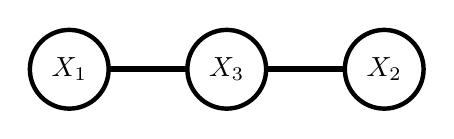
\begin{tikzpicture}[scale = 0.5]
\draw[black][fill=white,ultra thick](0,0)circle[radius=1];
\draw[black][fill=white,ultra thick](4,0)circle[radius=1];
\draw[black][fill=white,ultra thick](8,0)circle[radius=1];
\node at (0,0) [black][thick][scale=1]{$X_{1}$};
\node at (4,0) [black][thick][scale=1]{$X_{3}$};
\node at (8,0) [black][thick][scale=1]{$X_{2}$};
\draw [line width=2][-][black](1,0)--(3,0);
\draw [line width=2][-][black](5,0)--(7,0);
\end{tikzpicture}
\end{figure}

Problem b:
The inverse of $\Sigma$ contains no zero element, hence no conditional independency. Therefore there have to be edges between any two vertexes.
\begin{figure}[h]
\small
\centering
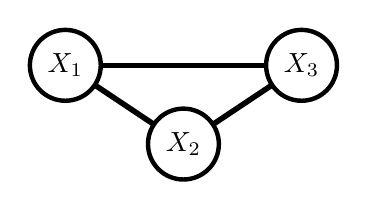
\begin{tikzpicture}[scale = 0.5]
\draw[black][fill=white,ultra thick](0,0)circle[radius=0.9];
\draw[black][fill=white,ultra thick](6,0)circle[radius=0.9];
\draw[black][fill=white,ultra thick](3,-2)circle[radius=0.9];
\node at (0,0) [black][thick][scale=1]{$X_{1}$};
\node at (6,0) [black][thick][scale=1]{$X_{3}$};
\node at (3,-2) [black][thick][scale=1]{$X_{2}$};
\draw [line width=2][-][black](0.75,-0.5)--(2.25,-1.5);
\draw [line width=2][-][black](5.25,-0.5)--(3.75,-1.5);
\draw [line width=2][-][black](0.9,0)--(5.1,0);
\end{tikzpicture}
\end{figure}

This model also cancels the marginal independency $X_{1}\perp X_{3}$. But it is possible to model this set of properties by Bayesian network with two directed edges $X_{1}\rightarrow X_{2}$ and $X_{3} \rightarrow X_{2}$.

Problem c:
Consider the terms inside the exponential:
$$-\frac{1}{2}\left\{ x_{1}^{2} + (x_{2}-x_{1})^{2} + (x_{3}-x_{2}^{2}) \right\}$$

It is easy to see the precision matrix and covariance matrix take:
$$\Lambda=\begin{pmatrix}2 & -1 & 0 \\ -1 & 2 & -1 \\ 0 & -1 & 1\\ \end{pmatrix},\Sigma = \begin{pmatrix}1 & 1 & 1 \\ 1 & 2 & 2\\ 1 & 2 & 3\\ \end{pmatrix}$$

Problem d:
The only independency is $X_{1}\perp X_{3} | X_{2}$:
\begin{figure}[h]
\small
\centering
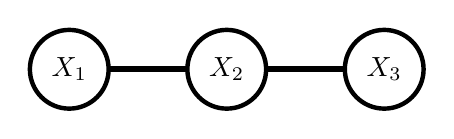
\begin{tikzpicture}[scale = 0.5]
\draw[black][fill=white,ultra thick](0,0)circle[radius=1];
\draw[black][fill=white,ultra thick](4,0)circle[radius=1];
\draw[black][fill=white,ultra thick](8,0)circle[radius=1];
\node at (0,0) [black][thick][scale=1]{$X_{1}$};
\node at (4,0) [black][thick][scale=1]{$X_{2}$};
\node at (8,0) [black][thick][scale=1]{$X_{3}$};
\draw [line width=2][-][black](1,0)--(3,0);
\draw [line width=2][-][black](5,0)--(7,0);
\end{tikzpicture}
\end{figure}

\subsection{Independencies in Gaussian graphical models}
Problem a and b:

This PGM implies $X_{1} \perp X_{3}|X_{2}$, hence we are looking for a precision matrix with $\Lambda_{1,3}=0$, thus C and D meet the condition. On the other hand, $(A^{-1})_{1,3}=(B^{-1})_{1,3}=0$. So A and B are candidates for covariance matrix.

Problem c and d:

This PGM tells that $X_{1} \perp X_{3}$. Hence C and D can be covariance matrix, A and B can be precision matrix.

The only possible PGM is:
\begin{figure}[h]
\small
\centering
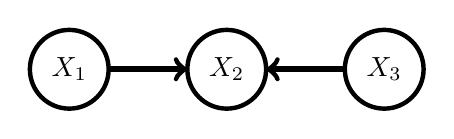
\begin{tikzpicture}[scale = 0.5]
\draw[black][fill=white,ultra thick](0,0)circle[radius=1];
\draw[black][fill=white,ultra thick](4,0)circle[radius=1];
\draw[black][fill=white,ultra thick](8,0)circle[radius=1];
\node at (0,0) [black][thick][scale=1]{$X_{1}$};
\node at (4,0) [black][thick][scale=1]{$X_{2}$};
\node at (8,0) [black][thick][scale=1]{$X_{3}$};
\draw [line width=2][->][black](1,0)--(3,0);
\draw [line width=2][<-][black](5,0)--(7,0);
\end{tikzpicture}
\end{figure}

Problem e:

The answer can be derived from the conclusion of marginal Gaussian directly, A is true while B not.

\subsection{Cost of training MRFs and CRFs}
The answer are generally:
$$O(r(Nc+1))$$

and
$$O(r(Nc+N))$$

\subsection{Full conditional in an Ising model}
Straightforwardly(we have omitted $\theta$ from condition w.l.o.g):
\begin{align}
p(x_{k}=1|\textbf{x}_{-k})=&\frac{p(x_{k}=1,\textbf{x}_{-k})}{p(\textbf{x}_{-k})} \nonumber \\
=&\frac{p(x_{k}=1,\textbf{x}_{-k})}{p(x_{k}=0,\textbf{x}_{-k})+p(x_{k}=1,\textbf{x}_{-k})} \nonumber \\
=&\frac{1}{1+\frac{p(x_{k}=0,\textbf{x}_{-k})}{p(x_{k}=1,\textbf{x}_{-k})}} \nonumber \\
=&\frac{1}{1+\frac{\exp(h_{k}\cdot 0)\prod_{<k,i>}\exp(J_{k,i}\cdot 0)}{\exp(h_{k}\cdot 1)\prod_{<k,i>}\exp(J_{k,i}\cdot x_{i})}} \nonumber \\
=&\sigma(h_{k}+\sum_{i=1,i\neq k}^{n}J_{k,i}x_{i}) \nonumber
\end{align}

When using denotation $x=\left\{ 0,1 \right\}$, the full conditional becomes:
$$p(x_{k}=1|\textbf{x}_{-k})\sigma(2\cdot (h_{k}+\sum_{i=1,i\neq k}^{n}J_{k,i}x_{i})) $$

\newpage
\section{Exact inference for graphical models}
\subsection{Variable elimination}
Where tf is the figure?!

\subsection{Gaussian times Gaussian is Gaussian}
We have:
\begin{align}
\ &N(x|\mu_{1},\lambda_{1}^{-1})\times N{N}(x|\mu_{2},\lambda_{2}^{-1})\nonumber \\
 =&\frac{\sqrt{\lambda_{1}\lambda_{2}}}{2\pi}\exp\left\{ -\frac{\lambda_{1}}{2}(x-\mu_{1})^{2}-\frac{\lambda_{2}}{2}(x-\mu_{2})^{2}  \right\}\nonumber \\
=& \frac{\sqrt{\lambda_{1}\lambda_{2}}}{2\pi} \exp\left\{ -\frac{\lambda_{1}+\lambda_{2}}{2}x^{2}+(\lambda_{1}\mu_{1}+\lambda_{2}\mu_{2})x-\frac{\lambda_{1}\mu_{1}^{2}+\lambda_{2}\mu_{2}^{2}}{2} \right\}  \nonumber
\end{align}

By completing the square:
\begin{align}
\ &\exp\left\{ -\frac{\lambda_{1}+\lambda_{2}}{2}x^{2}+(\lambda_{1}\mu_{1}+\lambda_{2}\mu_{2})x-\frac{\lambda_{1}\mu_{1}^{2}+\lambda_{2}\mu_{2}^{2}}{2} \right\} \nonumber \\
=&c\cdot \exp{-\frac{\lambda}{2}(x-\mu)^{2}}\nonumber
\end{align}

Where:
$$\lambda = \lambda_{1}+\lambda_{2}$$
$$\mu = \lambda^{-1}(\lambda_{1}\mu_{1}+\lambda_{2}\mu_{2})$$

The constant factor $c$ can be obtained by computing the constant terms inside the exponential.

\subsection{Message passing on a tree}
Problem a:

It is easy to see after variable elimination:
$$p(X_{2}=50) = \sum_{G_{1}}\sum_{G_{2}}p(G_{1})p(G_{2}|G_{1})p(X_{2}=50|G_{2})$$
$$p(G_{1}=1,X_{2}=50)=p(G_{1})\sum_{G_{2}}p(G_{2}|G_{1}=1)p(X_{2}=50|G_{2})$$

Thus:
$$p(G_{1}=1|X_{2}=50)=\frac{0.45+0.05\cdot \exp(-5)}{0.5 + 0.5 \cdot \exp(-5)}\approx 0.9$$

Problem b(here $X$ denotes $X_{2}$ or $X_{3}$):

\begin{align}
\ &p(G_{1}=1|X_{2}=50,X_{3}=50)\nonumber \\
 = &\frac{p(G_{1}=1,X_{2}=50,X_{3}=50)}{p(X_{2}=50,X_{3}=50)}\nonumber \\
=&\frac{p(G_{1}=1)p(X_{2}|G_{1}=1)p(X_{3}|G_{1}=1)}{p(G_{1}=0)p(X_{2}|G_{1}=0)p(X_{3}|G_{1}=0)+p(G_{1}=1)p(X_{2}|G_{1}=1)p(X_{3}|G_{1}=1)}\nonumber \\
=&\frac{p(X=50|G_{1}=1)^{2}}{p(X=50|G_{1}=0)^{2}+p(X=50|G_{1}=1)^{2}} \nonumber \\
\approx& \frac{0.9^{2}}{0.1^{2}+0.9^{2}} \approx 0.99 \nonumber
\end{align}

Extra evidence makes the belief in $G_{1}=1$ firmer.

Problem c:

The answer to problem c is symmetric to that to problem b, $p(G_{1}=0|X_{2}=60, X_{3}=60) \approx 0.99$.

Problem d:

Using the same pattern of analysis from Problem b, we have:
$$p(G_{1}=1|X_{2}=50, X_{3}=60)$$
$$=\frac{p(X=50|G_{1}=1)p(X=60|G_{1}=1)}{p(X=50|G_{1}=0)p(X=60|G_{1}=0)+p(X=50|G_{1}=1)p(X=60|G_{1}=1)}$$

Notice we have:
$$p(X=50|G_{1}=1)=p(X=60|G_{1}=0)$$
$$p(X=50|G_{1}=0)=p(X=60|G_{1}=1)$$

Hence:
$$P(G_{1}=1|X_{2}=50,X_{3}=60)=0.5$$

In this case, $X_{2}$ and $X_{3}$ have equal strength as evidence and their effects achieve a balance so they provide not enough information to distort the prior knowledge.

\subsection{Inference in 2D lattice MRFs}
Please refer to PGM:principals and techniques 11.4.1.


\newpage
\section{Variational inference}
\subsection{Laplace approximation to $p(\mu,\log \sigma|D)$ for a univariate Gaussian}
Laplace approximation equals representing $f(\mu,l)=\log p(\mu,l=\log \sigma|D)$ with second-order Taylor expansion. We have:
\begin{align}
\log p(\mu,l|D)=&\log p(\mu,l,D)-\log p(D)\nonumber \\
=&\log p(\mu,l) + \log p(D|\mu,l) + c \nonumber \\
=&\log p(D|\mu,l) + c \nonumber \\
=&\sum_{n=1}^{N}\log \frac{1}{\sqrt{2\pi\sigma^{2}}}\exp\left\{-\frac{1}{2\sigma^{2}}(y_{n}-\mu)^{2}  \right\}+c \nonumber \\
=&-N\log \sigma+\sum_{n=1}^{N}-\frac{1}{2\sigma^{2}}(y_{n}-\mu)^{2}+c\nonumber \\
=&-N\cdot l+\frac{1}{2}\frac{1}{\exp\left\{2\cdot l\right\}}\sum_{n=1}^{N}(y_{n}-\mu)^{2}+c \nonumber
\end{align}

Thus we derive:
\begin{align}
\frac{\partial \log p(\mu,l|D)}{\partial \mu}=&\frac{1}{2}\frac{1}{\exp\left\{2\cdot l\right\}}\sum_{n=1}^{N}2\cdot (y_{n}-\mu) \nonumber \\
=&\frac{N}{\sigma^{2}}\cdot (\bar{y}-\mu)\nonumber \\
\frac{\partial \log p(\mu,l|D)}{\partial l}=&-N + \frac{1}{2}\sum_{n=1}^{N}(y_{n}-\mu)^{2}\cdot (-2)\cdot \frac{1}{\exp\left\{2\cdot l  \right\}} \nonumber \\
=&-N+\frac{1}{\sigma^{2}}\sum_{n=1}^{N}(y_{n}-\mu)^{2} \nonumber \\
\frac{\partial^{2} \log p(\mu,l|D)}{\partial \mu^{2}}=&-\frac{N}{\sigma^{2}} \nonumber \\
\frac{\partial^{2} \log p(\mu,l|D)}{\partial l^{2}}=&-\frac{2}{\sigma^{2}}\sum_{n=1}^{N}(y_{n}-\mu)^{2} \nonumber \\
\frac{\partial^{2} \log p(\mu,l|D)}{\partial \mu \partial l}=&N\cdot (\bar{y}-\mu)\cdot (-2) \cdot \frac{1}{\sigma^{2}} \nonumber
\end{align}

For approximation, $p(\mu,l) \approx N(\mu, \Sigma)$ with:
$$\Sigma = \begin{pmatrix} \frac{\partial^{2} \log p(\mu,l|D)}{\partial \mu^{2}} & \frac{\partial^{2} \log p(\mu,l|D)}{\partial l^{2}} \\ \frac{\partial^{2} \log p(\mu,l|D)}{\partial l^{2}} &  \frac{\partial^{2} \log p(\mu,l|D)}{\partial \mu \partial l} \\ \end{pmatrix}^{-1}$$
$$\mu = \Sigma \begin{pmatrix} \frac{\partial \log p(\mu,l|D)}{\partial \mu} \\ \frac{\partial \log p(\mu,l|D)}{\partial l}  \end{pmatrix}$$

\subsection{Laplace approximation to normal-gamma}
This is the same with exercise 21.1 when the prior is uniformative. We formally substitute:
\begin{align}
\sum_{n=1}^{N}(y_{n}-\mu)^{2}=& \sum_{n=1}^{N}((y_{n}-\bar{y})-(\mu-\bar{y}))^{2} \nonumber \\
=&\sum_{n=1}^{N}(y_{n}-\bar{y})^{2} + \sum_{n=1}^{N}(\mu-\bar{y})^{2} + 2(\mu-\bar{y})\cdot\sum_{n=1}^{N}(y_{n}-\bar{y})\nonumber \\
=&Ns^{2}+N(\mu-\bar{y})^{2} \nonumber
\end{align}

Where $s^{2}=\frac{1}{N}\sum_{n=1}^{N}(y_{n}-\bar{y})^{2}$

Conclusions in all problems a, b and c are included in the previous solution.

\subsection{Variational lower bound for VB for univariate Gaussian}
What left in section 21.5.1.6 is the derivation for 21.86 to 21.91. We omit the derivation for entropy for Gaussian and moments, which can be found in any information theory textbook. Now we derive the $\mathbb{E}[\ln x|x \sim Ga(a,b)]$, which can therefore yields to the entropy for a Gamma distribution.

We know that Gamma distribution is an exponential family distribution:
\begin{align}
Ga(x|a,b)=&\frac{b^{a}}{\Gamma(a)}x^{a-1}\exp\left\{-b\cdot x \right\}\nonumber \\
\propto& \exp\left\{-b\cdot x+(a-1) \ln x  \right\} \nonumber\\
=&\exp\left\{ \phi(x)^{T}\theta \right\}\nonumber
\end{align}

The sufficient statistics is $\phi(x)=(x,\ln x)^{T}$ and natural parameter is given by $\theta = (-b,a-1)^{T}$. Thus Gamma distribution can be seen as the maximum entropy distribution under constraints on $x$ and $\ln x$.

The culumant function is given by:
\begin{align}
A(\theta)=& \log Z(\theta)\nonumber \\
=&\log \frac{\Gamma(a)}{b^{a}} \nonumber \\
=&\log \Gamma(a) - a \log b \nonumber
\end{align}

The expectation of sufficient statistics is given by the derivative of cumulant function, therefore:
$$\mathbb{E}[\ln x] = \frac{\partial A}{\partial (a-1)} = \frac{\Gamma'(a)}{\Gamma(a)}-\log b$$

According to defintion $\psi(a)=\frac{\Gamma'(a)}{\Gamma(a)}$:
$$\mathbb{E}[\ln x] = \psi(a)-\log b$$

The rest derivations are completed or trivial.

\subsection{Variational lower bound for VB for GMMs}
The lower bound is given by:
\begin{align}
\mathbb{E}_{q}[\log \frac{p(\theta,D)}{q(\theta)}] =& \mathbb{E}_{q}[\log p(\theta,D)] -\mathbb{E}_{q}[q(\theta)]\nonumber \\
=&\mathbb{E}_{q}[\log p(D|\theta)]+\mathbb{E}_{q}[\log p(\theta)]+\mathbb{E}_{q}[\log q(\theta)] \nonumber \\
=&\mathbb{E}[\log p(\textbf{x}|\textbf{z},\mu,\Lambda,\pi)] + \mathbb{E}[\log p(\textbf{z},\mu,\Lambda,\pi)]\nonumber \\
\ &-\mathbb{E}[\log q(\textbf{z},\mu,\Lambda,\pi)]\nonumber \\
=&\mathbb{E}[\log p(\textbf{x}|\textbf{z},\mu,\Lambda,\pi)] + \mathbb{E}[\log p(\textbf{z}|\pi)] + \mathbb{E}[\log p(\pi)] + \mathbb{E}[\log p(\mu, \Lambda)] \nonumber \\
\ &+ \mathbb{E}[\log q(\textbf{z})] + \mathbb{E}[\log q(\pi)] + \mathbb{E}[\log q(\mu,\Lambda)]\nonumber
\end{align}

We are now showing 21.209 to 21.215.

For 21.209:
\begin{align}
\mathbb{E}[\log p(\textbf{x}|\textbf{z},\mu,\Lambda)]=& \mathbb{E}_{q(\textbf{z})q(\mu,\Lambda)}[\log p(\textbf{x}|\textbf{z},\mu,\Lambda)] \nonumber \\
=& \sum_{n}\sum_{k}\mathbb{E}_{q(\textbf{z})q(\mu,\Lambda)}[-\frac{D}{2}\log 2\pi + \frac{1}{2}\log |\Lambda_{k}|-\frac{1}{2}(x_{n}-\mu_{k})^{T}\Lambda_{k}(x_{n}-\mu_{k})]\nonumber
\end{align}

Using 21.132 and converting summing by average $\bar{x}_{k}$ yields to solution.

For 21.210:
\begin{align}
\mathbb{E}[\log p(\textbf{z}|\pi)]=&\mathbb{E}_{q(\textbf{z})q(\pi)}[\log p(\textbf{z}|\pi)]\nonumber \\
=&\mathbb{E}_{q(\textbf{z})q(\pi)}[\log \prod_{n=1}^{N}\prod_{k=1}^{K}\pi_{k}^{z_{nk}}] \nonumber \\
=&\sum_{n=1}^{N}\sum_{k=1}^{K}\mathbb{E}_{q(\textbf{z})q(\pi)}[z_{nk}\log \pi_{k}]\nonumber \\
=&\sum_{n=1}^{N}\sum_{k=1}^{K}\mathbb{E}_{q(\textbf{z})}[z_{nk}]\mathbb{E}_{q(\pi)}[\log \pi_{k}]\nonumber \\
=&\sum_{n=1}^{N}\sum_{k=1}^{K}r_{nk}\log \bar{\pi}_{k}\nonumber
\end{align}

For 21.211:
\begin{align}
\mathbb{E}[\log p(\pi)]=&\mathbb{E}_{q(\pi)}[\log p(\pi)] \nonumber \\
=&\mathbb{E}_{q(\pi)}[\log (C\cdot \prod_{k=1}^{K}\pi_{k}^{\alpha_{0}-1})]\nonumber \\
=&\ln C + (\alpha_{0}-1)\sum_{k=1}^{K}\log \bar{\pi}_{k} \nonumber
\end{align}

For 21.212:
\begin{align}
\mathbb{E}[\log p(\mu,\Lambda)]=&\mathbb{E}_{q(\mu,\Lambda)}[\log p(\mu,\Lambda)] \nonumber \\
=&\mathbb{E}_{q(\mu,\Lambda)}[\log \prod_{k=1}^{K}Wi(\Lambda_{k}|L_{0},v_{0})\cdot N(\mu_{k}|m_{0},(\beta_{0}\Lambda_{k})^{-1}]\nonumber \\
=&\sum_{k=1}^{K}\mathbb{E}_{q(\mu,\Lambda)}[ \log C + \frac{1}{2}(v_{0}-D-1)\log |\Lambda_{k}| -\frac{1}{2}tr\left\{ \Lambda_{k}L_{0}^{-1} \right\}\nonumber \\
\ & - \frac{D}{2}\log 2 \pi - \frac{1}{2}\log |\beta_{0}\Lambda_{k}| -\frac{1}{2}(\mu_{k}-m_{0})^{T}(\beta_{0}\Lambda_{k})(\mu_{k}-m_{0}) ]\nonumber
\end{align}

Using 21.131 to expand the expected value of the quadratic form and using the fact that the mean of a Wi distribution is $v_{k}L_{k}$ and we are done.

For 21.213:
\begin{align}
\mathbb{E}[\log q(\textbf{z})]=& \mathbb{E}_{q(\textbf{z})}[\log q(\textbf{z})] \nonumber \\
=&\mathbb{E}_{q(\textbf{z})}[\sum_{i}\sum_{k}z_{ik}\log r_{ik}]\nonumber \\
=&\sum_{i}\sum_{k} \mathbb{E}_{q(\textbf{z})}[z_{ik}]\log r_{ik}\nonumber \\
=& \sum_{i}\sum_{k} r_{ik}\log r_{ik}\nonumber
\end{align}

For 21.214:
\begin{align}
\mathbb{E}[\log q(\pi)]=&\mathbb{E}_{q(\pi)}[\log q(\pi)] \nonumber \\
=&\mathbb{E}_{q(\pi)}[\log C + \sum_{k=1}^{K}(\alpha_{k}-1)\log \pi_{k}] \nonumber \\
=&\log C + \sum_{k}(\alpha_{k}-1)\log \bar{\pi}_{k} \nonumber
\end{align}

For 21.215:
\begin{align}
\mathbb{E}[\log q(\mu,\Lambda)]=& \mathbb{E}_{q(\mu,\Lambda)}[\log q(\mu,\Lambda)] \nonumber \\
=&\sum_{k}\mathbb{E}_{q(\mu,\Lambda)}[\log q(\Lambda_{k})-\frac{D}{2}\log 2\pi +\frac{1}{2}\log |\beta_{k}\Lambda_{k}|\nonumber \\
\ &-\frac{1}{2}(\mu_{k}-m_{k})^{T}(\beta_{k}\Lambda_{k})(\mu_{k}-m_{k})  ]\nonumber
\end{align}

Using 21.132 to expand the quadratic form to give $\mathbb{E}[(\mu_{k}-m_{k})^{T}(\beta_{k}\Lambda_{k})(\mu_{k}-m_{k})]=D$

\subsection{Derivation of $\mathbb{E}[\log \pi_{k}]$} under a Dirichlet distribution
Dirichlet distribution is an exponential family distribution, we have:
$$\phi(\pi)=(\log \pi_{1},\log \pi_{2},...\log \pi_{K})$$
$$\theta=\alpha$$

The cumulant function is:
$$A(\alpha)=\log B(\alpha) = \sum_{i=1}^{K}\log \Gamma(\alpha_{i})-\log \Gamma(\sum_{i=1}^{K}\alpha_{i})$$

And:
$$\mathbb{E}[\log \pi_{k}]=\frac{\partial A(\alpha)}{\partial \alpha_{k}} = \frac{\Gamma'(\alpha_{k})}{\Gamma(\alpha_{k})}- \frac{\Gamma'(\sum_{i=1}^{K}\alpha_{k})}{\Gamma(\sum_{i=1}^{K}\alpha_{k})}=\psi(\alpha_{k})-\psi(\sum_{i=1}^{K}\alpha_{i})$$

Take exponential on both sides:
$$\exp(\mathbb{E}[\log \pi_{k}])=\exp(\psi(\alpha_{k})-\psi(\sum_{i=1}^{K}\alpha_{k}))=\frac{\exp(\alpha_{k})}{\exp(\sum_{i=1}^{K}\alpha_{i})}$$

\subsection{Alternative derivation of the mean field updates for the Ising model}
This is no different than applying the procedure in section 21.3.1 before derivating updates, hence omitted.

\subsection{Forwards vs reverse KL divergence}
We have:
\begin{align}
KL(p(x,y)||q(x,y))=&\mathbb{E}_{p(x,y)}[\log \frac{p(x,y)}{q(x,y)}]\nonumber \\
=&\sum_{x,y}p(x,y)\log p(x,y)-\sum_{x,y}p(x,y)\log q(x)-\sum_{x,y}p(x,y)\log q(y) \nonumber \\
=&\sum_{x,y}p(x,y)\log p(x,y)-\sum_{x}(\sum_{y}p(x,y))\log q(x)-\sum{y}(\sum_{x}p(x,y))\log q(q) \nonumber \\
=&H(p(x,y))-H(p(x))-H(p(y))+KL(p(x)||q(x))+KL(p(y)||q(y))\nonumber \\
=& constant + KL(p(x)||q(x))+KL(p(y)||q(y))\nonumber
\end{align}

Thus the optimal approximation is $q(x)=p(x)$ and $q(y)=p(y)$.

We skip the practical part.

\subsection{Derivation of the structured mean field updates for FHMM}
According to the conclusion from mean-field varitional methods, we have:
$$E(\textbf{x}_{m})=\mathbb{E}_{q/m}[E(\bar{p}(\textbf{x}_{m}))]$$

Thus:
$$-\sum_{t=1}^{T}\sum_{k=1}^{K}x_{t,m,k}\tilde{\epsilon}_{t,m,k}=\frac{1}{2}\mathbb{E}[\sum_{t=1}^{T}(\textbf{y}_{t}-\sum_{l\neq m}^{M}W_{l}\textbf{x}_{t,m})^{T}\Sigma^{-1}(\textbf{y}_{t}-\sum_{l\neq m}^{M}W_{l}\textbf{x}_{t,m})]+C$$

Comparing the coefficient of $x_{t,m,k}$ (i.e. setting $x_{t,m,k}$ to 1) ends in:
$$\tilde{\epsilon}_{t,m,k}=W^{T}_{m}\Sigma^{-1}(\textbf{y}_{t}-\sum_{l\neq m}W_{l}\mathbb{E}[\textbf{x}_{t,l}])-\frac{1}{2}(W^{T}_{m}\Sigma^{-1}W_{m})_{k,k}$$

Write into matrix form yields to 21.62.

\subsection{Variational EM for binary FA with sigmoid link}
Refer to "Probabilistic Visualisation of High-Dimensional Binary Data, Tipping, 1998".

\subsection{VB for binary FA with probit link}
The major difference in using probit link is the uncontinuous likelihood caused by $p(y_{i}=1|z_{i})=\mathbb{I}(z_{i}>0)$. In the context of hiding $\textbf{X}$, we assume Gaussian prior on $\textbf{X}$, $\textbf{W}$ and $\textbf{Z}$. The approximation takes the form:
$$q(\textbf{X},\textbf{Z},\textbf{W})=\prod_{l=1}^{L}q(\textbf{w}_{l})\prod_{i=1}^{N}q(\textbf{x}_{i})q(z_{i})$$

It is a mean-field approximation, hence in an algorithm similari to EM, we are to update the distribution of $\textbf{X}$, $\textbf{Z}$ and $\textbf{W}$ stepwise.

For variable $\textbf{X}$, we have:
\begin{align}
\log q(\textbf{x}_{i})=&\mathbb{E}_{q(\textbf{z}_{i})q(\textbf{w})}[\log p(\textbf{x}_{i},\textbf{w},z_{i},y_{i})] \nonumber \\
=& \mathbb{E}_{q(\textbf{z}_{i})q(\textbf{w})}[\log p(\textbf{x}_{i})+\log p(\textbf{w})+\log p(z_{i}|\textbf{w}_{i},\textbf{w})+\log p(y_{i}|z_{i})] \nonumber
\end{align}

Given the likelihood form, for $i$ corresponding to $y_{i}=1$, $q(z_{i})$ have to be a truncated one, i.e. we only consider the expectations in the form $\mathbb{E}[z|z>\mu]$ and $\mathbb{E}[z^{2}|z>\mu]$.

$\log q(\textbf{x}_{i}) = -\frac{1}{2}\textbf{x}_{i}^{T}\Lambda_{1}\textbf{x}_{i}-\frac{1}{2}\mathbb{E}[z^{2}]-\frac{1}{2}\textbf{x}^{T}_{i} \mathbb{E}[\textbf{w}\textbf{w}^{T}]\textbf{x}_{i}+\mathbb{E}[z]\mathbb{E}[\textbf{w}]^{T}\textbf{x}_{i}$

Where $\Lambda_{1}$ is the covariance of $\textbf{x}_{i}$'s prior distribution, $\mathbb{E}[\textbf{w}\textbf{w}^{T}]$ can be calculated given the Gaussian form of $q(\textbf{w})$, and truncated expectations $\mathbb{E}[z]$ and $\mathbb{E}[z^{2}]$ can be obtained from solutions to exercise 11.15. It is obvious that $q(\textbf{x}_{i})$ is a Gaussian.

The update for $\textbf{w}$ is similar to that for $\textbf{x}_{i}$ as long as they play symmetric roles in likelihood. The only difference is we have to sum over $i$ when updating $\textbf{w}$.

At last we update $z_{i}$:
$$\log q(z_{i})=\mathbb{E}_{q(\textbf{x}_{i})q(\textbf{w})}[\log p(z_{i}|\textbf{x}_{i},\textbf{w})+\log p(y_{i}|z_{i})]$$

Inside the expectation we have:
$$-\frac{1}{2}z_{i}^{2}+\mathbb{E}[\textbf{w}]^{T}\mathbb{E}[\textbf{x}]z_{i}+c$$

Therefore $q(z_{i})$ again takes a Gaussian form.

\end{document}

%插入图片格式:
%\begin{figure}[h]
%\small
%\centering
%\includegraphics[width=6cm]{./gaussian/Maxwell_Laplace_Gaussian_.jpg}
%\caption{拉普拉斯近似,$\sigma^{2}=0.3$} \label{fig:aa}
%\end{figure}
